


\documentclass[11pt,titlepage,twoside]{article}\usepackage[]{graphicx}\usepackage[table]{xcolor}
% maxwidth is the original width if it is less than linewidth
% otherwise use linewidth (to make sure the graphics do not exceed the margin)
\makeatletter
\def\maxwidth{ %
  \ifdim\Gin@nat@width>\linewidth
    \linewidth
  \else
    \Gin@nat@width
  \fi
}
\makeatother

\definecolor{fgcolor}{rgb}{0.345, 0.345, 0.345}
\newcommand{\hlnum}[1]{\textcolor[rgb]{0.686,0.059,0.569}{#1}}%
\newcommand{\hlsng}[1]{\textcolor[rgb]{0.192,0.494,0.8}{#1}}%
\newcommand{\hlcom}[1]{\textcolor[rgb]{0.678,0.584,0.686}{\textit{#1}}}%
\newcommand{\hlopt}[1]{\textcolor[rgb]{0,0,0}{#1}}%
\newcommand{\hldef}[1]{\textcolor[rgb]{0.345,0.345,0.345}{#1}}%
\newcommand{\hlkwa}[1]{\textcolor[rgb]{0.161,0.373,0.58}{\textbf{#1}}}%
\newcommand{\hlkwb}[1]{\textcolor[rgb]{0.69,0.353,0.396}{#1}}%
\newcommand{\hlkwc}[1]{\textcolor[rgb]{0.333,0.667,0.333}{#1}}%
\newcommand{\hlkwd}[1]{\textcolor[rgb]{0.737,0.353,0.396}{\textbf{#1}}}%
\let\hlipl\hlkwb

\usepackage{framed}
\makeatletter
\newenvironment{kframe}{%
 \def\at@end@of@kframe{}%
 \ifinner\ifhmode%
  \def\at@end@of@kframe{\end{minipage}}%
  \begin{minipage}{\columnwidth}%
 \fi\fi%
 \def\FrameCommand##1{\hskip\@totalleftmargin \hskip-\fboxsep
 \colorbox{shadecolor}{##1}\hskip-\fboxsep
     % There is no \\@totalrightmargin, so:
     \hskip-\linewidth \hskip-\@totalleftmargin \hskip\columnwidth}%
 \MakeFramed {\advance\hsize-\width
   \@totalleftmargin\z@ \linewidth\hsize
   \@setminipage}}%
 {\par\unskip\endMakeFramed%
 \at@end@of@kframe}
\makeatother

\definecolor{shadecolor}{rgb}{.97, .97, .97}
\definecolor{messagecolor}{rgb}{0, 0, 0}
\definecolor{warningcolor}{rgb}{1, 0, 1}
\definecolor{errorcolor}{rgb}{1, 0, 0}
\newenvironment{knitrout}{}{} % an empty environment to be redefined in TeX

\usepackage{alltt}
\usepackage[a4paper, inner=1.5cm, outer=1.5cm, top=2cm, bottom=3cm]{geometry}

\usepackage[utf8]{inputenc} 
\usepackage[T1]{fontenc}
\usepackage[sort&compress]{natbib}
\usepackage[french]{babel}

\addto\captionsfrench{\def\tablename{Tableau}}
\addto\captionsfrench{\renewcommand*{\contentsname}{Sommaire:}}
\addto\captionsfrench{%
  \renewcommand{\listfigurename}{Liste des figures:}%
  \renewcommand{\listtablename}{Liste des tableaux:}%
  \renewcommand{\abstractname}{Résumé}%
}
\usepackage{caption}
\usepackage[labelsep=endash]{caption}
\usepackage{graphicx}
\usepackage{colortbl}
\usepackage{booktabs}
\usepackage{longtable}
\usepackage{array}
\usepackage{multirow}
\usepackage{wrapfig}
\usepackage{float}
\usepackage{pdflscape}
\usepackage{tabu}
\usepackage{threeparttable}
\usepackage{threeparttablex}
\usepackage[normalem]{ulem}
\usepackage{makecell}
\usepackage[table]{xcolor}
\usepackage{ae,aeguill}
\usepackage{subcaption}
\usepackage{gensymb}
\usepackage{authblk}
\usepackage{natbib}
\usepackage{xcolor}
\renewcommand\Authand{ et }
\renewcommand\Authands{ et }

\usepackage{textcomp}
\usepackage{hyperref}
\pdfstringdefDisableCommands{%
  \def\\{}%
  }
\hypersetup{ 
colorlinks=true, 
linkcolor=blue, 
citecolor=blue, 
filecolor=blue, 
urlcolor=blue, 
pdftitle= {Suivi et estimation du recrutement en anguille européenne sur le fleuve Seine\\ Année 2024 }, pdfauthor={Marangoni Lucas},
pdfsubject={stacomi},
 pdfkeywords={stacomi} {migrateurs} {Seine} {poissons}
}
\pdfoptionpdfminorversion=7
\renewcommand{\sectionmark}[1]{\markboth{}{\emph{\thesection~#1}}}
\renewcommand{\subsectionmark}[1]{\markboth{}{\emph{\thesubsection~#1}}}
\renewcommand{\subsubsectionmark}[1]{\markboth{}{\emph{\thesubsection~#1}}}

\makeatletter
    \def\@@and{et}
\makeatother

\usepackage{fancyhdr}
\pagestyle{fancy}
\fancyhf{}
\rhead{\rightmark}
\lfoot{\footnotesize{Suivi et estimation du recrutement en anguille européenne sur le fleuve Seine, année 2024}} %Insere un pied de page avec le texte a gauche.
\rfoot{\thepage}
\setlength{\headheight}{15pt}

\usepackage{pdfpages}
\usepackage{setspace}

%%%%%%%%%%%%%%%%%%%%%%%%%%%%%%%%%%%%%%%%%%%
%%%%%% CHUNK DE CHARGEMENT INITIAL  %%%%%%%
%%%%%%%%%%%%%%%%%%%%%%%%%%%%%%%%%%%%%%%%%%%



%% Makes a path to your graphics' folder.
\graphicspath{{image/}}

\title{Suivi et estimation du recrutement en anguille européenne sur le fleuve Seine,
année 2024}

\author[1]{Marangoni Lucas}
\affil[1]{Seine-Normandie Migrateurs, 11 cours Clemenceau 76100 Rouen}
\IfFileExists{upquote.sty}{\usepackage{upquote}}{}
\begin{document}

\hypersetup{pageanchor=false}

\begin{titlepage}

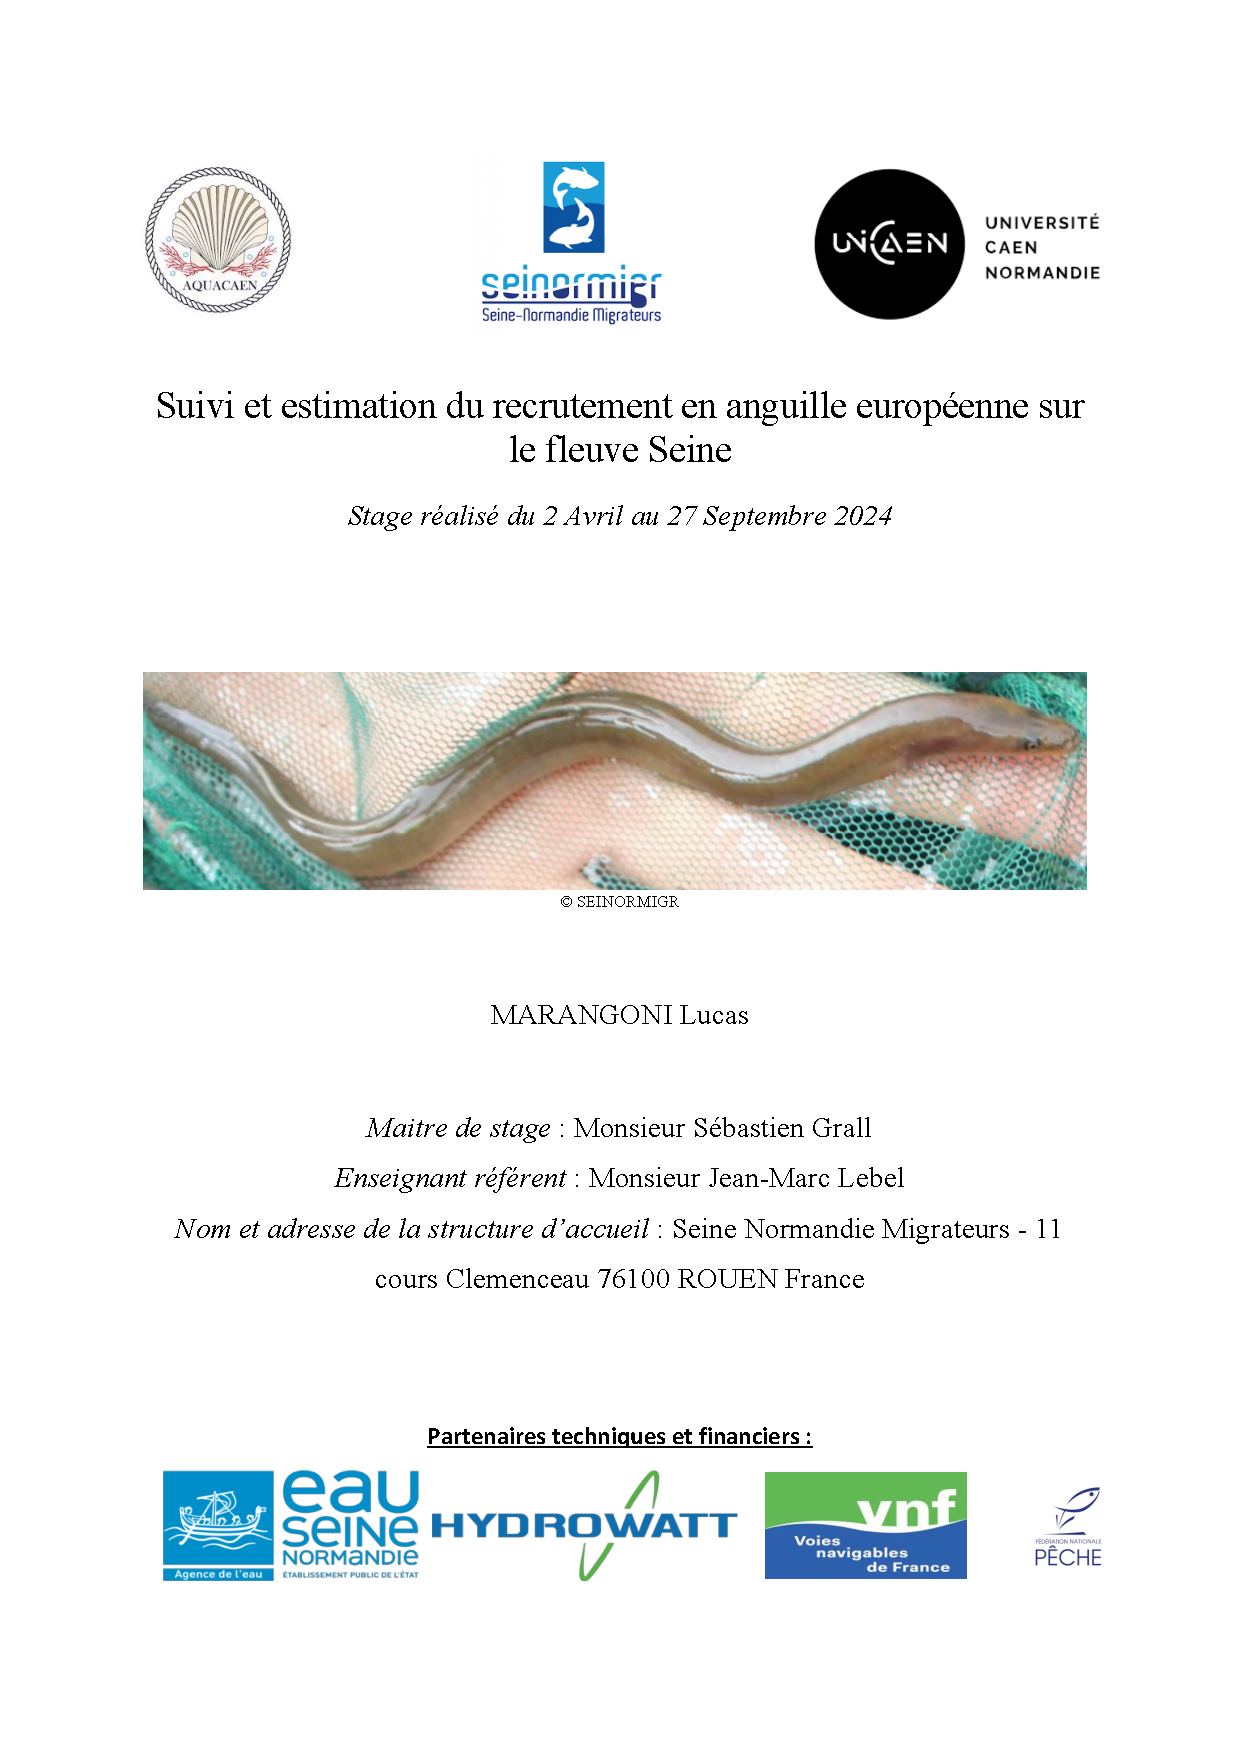
\includepdf[pages=-]{frontpage.pdf}

\end{titlepage}



\newpage
\thispagestyle{empty}
\strut
\newpage

\pagenumbering{roman} \setcounter{page}{1}

\maketitle

\begin{abstract}

Un suivi du recrutement de l’anguille européenne en Seine est réalisé depuis 2014 en rive gauche et 2018 en rive droite du barrage de Poses, premier ouvrage sur la Seine. Ce suivi a été mis en place dans le cadre du Plan National de Gestion Anguille (PGA). Pour cette année 2024, un total de 846 545 anguilles a été comptabilisé avec 90\% des individus en rive droite et 10\% des individus en rive gauche. La mise en place d’une rampe à anguille en rive droite a fortement augmenté les chiffres car l’accessibilité de la rampe en rive gauche est trop difficile à cause des courants issus de l’usine hydroélectrique. Les facteurs environnementaux jouent un rôle dans la montaison des anguilles. Cette année les résultats ont réussi a montré un impact significatif positif des températures de l’air et de l’eau fortement corrélées entre elles. Les débits et les niveaux d’eau étaient extrêmement élevés, cela a joué un rôle dans l’accessibilité des anguilles en venant modifier et contrer les courants de l’usine hydroélectrique. En complémentarité des dispositifs de piégeages, des flottangs ont été mis en place en aval des rampes visant à vérifier le bon fonctionnement des dispositifs. Une amélioration des chiffres est visible cette année mais nous ne pouvons pas qualifier la situation de satisfaisante comparé aux chiffres des années 80.
Mots-clés :  \textit{Anguilla Anguilla} ; Montaison ; Recrutement ; Rampe à anguille ; Seine


\end{abstract}

\newpage

\tableofcontents

\clearpage

\listoffigures

\listoftables

\hypersetup{pageanchor=false}

\clearpage

\pagenumbering{arabic} \setcounter{page}{1} 

\clearpage

\begin{center}
\textbf{Seine Normandie Migrateurs}
\end{center}

\addcontentsline{toc}{section}{Seine Normandie Migrateurs}

Péambule : Les informations présentées ci-dessous sont tirées du site internet : https://www.seinormigr.fr.

\vspace{0.5cm}
\underline{Présentation générale} : Seinormigr a été créé en 2007 sur une initiative du Président de la Fédération de la Seine-Maritime pour la Pêche et la Protection du Milieu Aquatique. 
L’association regroupe par adhésion les Fédérations départementales présentes sur le bassin Seine-Normandie afin de créer une seule et même continuité dans le suivi et la gestion des populations de poissons migrateurs. 
En 2011, elle est inscrite au Plan de Gestion des Poissons Migrateurs du bassin Seine-Normandie où elle siège en tant qu’inviter. 
En 2012, Seinormigr obtient son agrément d’association de protection de l’environnement par arrêté préfectoral du 13 décembre 2012. 
Puis en 2013, l'association est habilitée pour prendre part aux débats environnementaux se déroulant dans le cadre des instances consultatives régionales. 
Enfin en 2020, Seine-Normandie Migrateurs et Normandie Grands Migrateurs ont fusionné pour ne créer qu'une seule association grands migrateurs sur le territoire Seine-Normandie.
\vspace{0.5cm}

\underline{Missions} :

-	Contribuer à la connaissance, l’évaluation et au suivi des populations piscicoles amphihalines sur le bassin Seine-Normandie et la région Normandie.

-	Favoriser la valorisation et la gestion des grands migrateurs, notamment avec un porter à connaissance technique et scientifique qui soit visible et accessible en veillant au développement durable des pratiques halieutiques.

-	Participer et s’investir techniquement et/ou financièrement dans les projets de restauration des axes de circulation et des habitats de reproduction et de développement des poissons migrateurs en vue d’assurer leur sauvegarde et la recolonisation des cours d’eau.

-	Assister les maîtres d’ouvrages et les services instructeurs en matière technique et administrative dans tous les projets contribuant à l’accomplissement du cycle biologique des grands migrateurs.

-	Mener ou coordonner des études ou publications spécifiques en concertation avec les différents gestionnaires et pouvoir publics en appui aux décisions politiques locales de l’eau afin de démontrer le bénéfice de l’action à consentir à toutes les échelles des cours d’eau.

-	Participer à la définition et la mise en œuvre des objectifs de restauration des populations de poissons migrateurs au sein du COGEPOMI et de son PLAGEPOMI en collaboration étroite avec le secrétariat technique (DRIEE Île de France, Délégation de bassin) et les établissements publics de l’Etat (DREAL, AFB, Agence de l’Eau, DDTM, …).

-	Développer une large communication de synthèse des productions basées sur des données d’expertises, notamment à l’aide de mise à disposition d’outils de communication à différentes échelles des besoins qu’ils soient locaux, régionaux ou de bassins.
\vspace{0.5cm}

\underline{Territoires d’action} :  Seine Normandie Migrateurs fait partie des 8 associations migratrices présentent en France qui recouvrent les grands bassins français (Figure \ref{AM_National}). 
L’association regroupe par adhésion 18 Fédérations Départementales pour la Pêche et la Protection du Milieu Aquatique (FDAAPPMA), des Associations Agréées pour la Pêche et la Protection du Milieu Aquatique (AAPPMA), ainsi que des adhérents directs. 
Son territoire s’étend sur une superficie totale de 95 500 km², englobant près de 50 000 km de cours d’eau, composé d’une très grande partie du bassin versant de la Seine et de ceux des fleuves côtiers Normands. 

\vspace{0.5cm}

\begin{figure}[htpb]
\centering
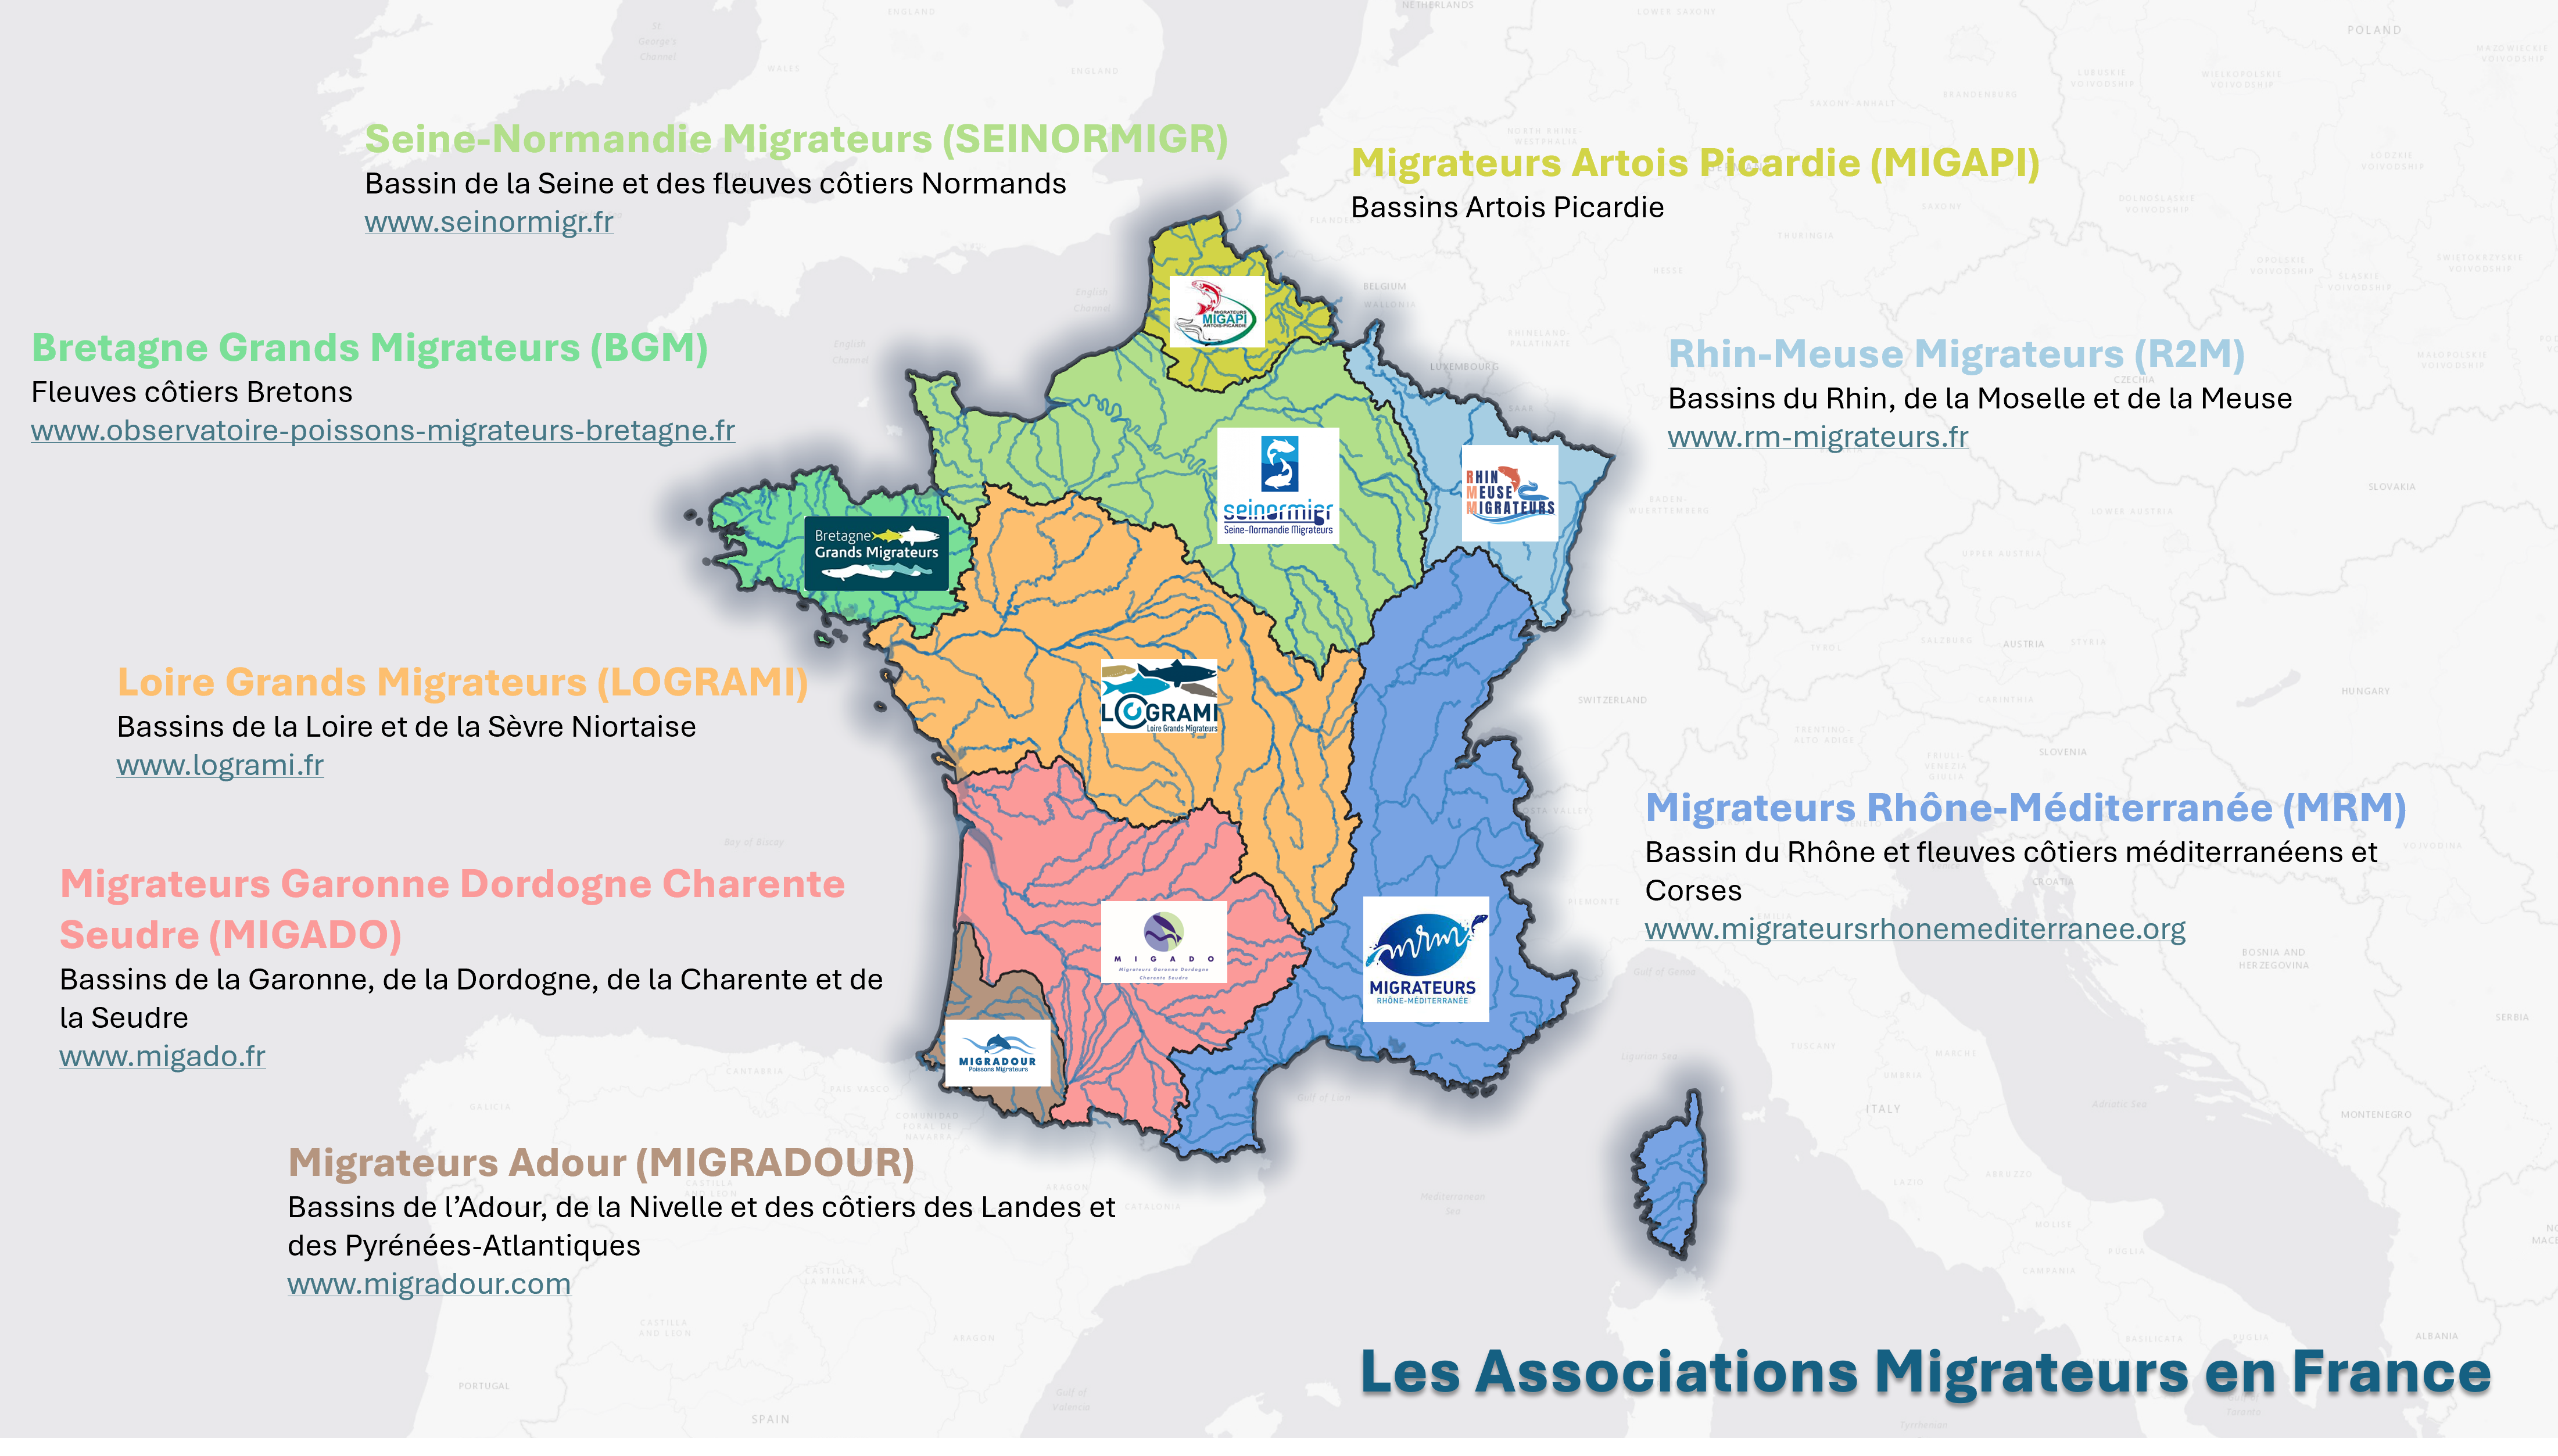
\includegraphics[width=\textwidth]{AM_National.png}
\caption{Associations migrateurs (AM) des grands bassins français (SEINORMIGR)}
\label{AM_National}
\end{figure}


\underline{Organisation} : Plus de 200 000 pêcheurs à travers 18 fédérations départementales pour la pêche et la protection des milieux aquatiques sont représentés par Seinormigr. 
L’association est dirigée par un conseil d’administration de 20 membres avec à sa tête le Président M. Martial CHOUQUET, également président de la FDPPMA de l’Eure. Aujourd’hui l’équipe technique est composée de 6 salariés permanents répartis sur deux antennes Rouen (76) et Mondeville (14) (Figure \ref{Organigramme_Seinormigr}) :

\begin{figure}[htpb]
\centering
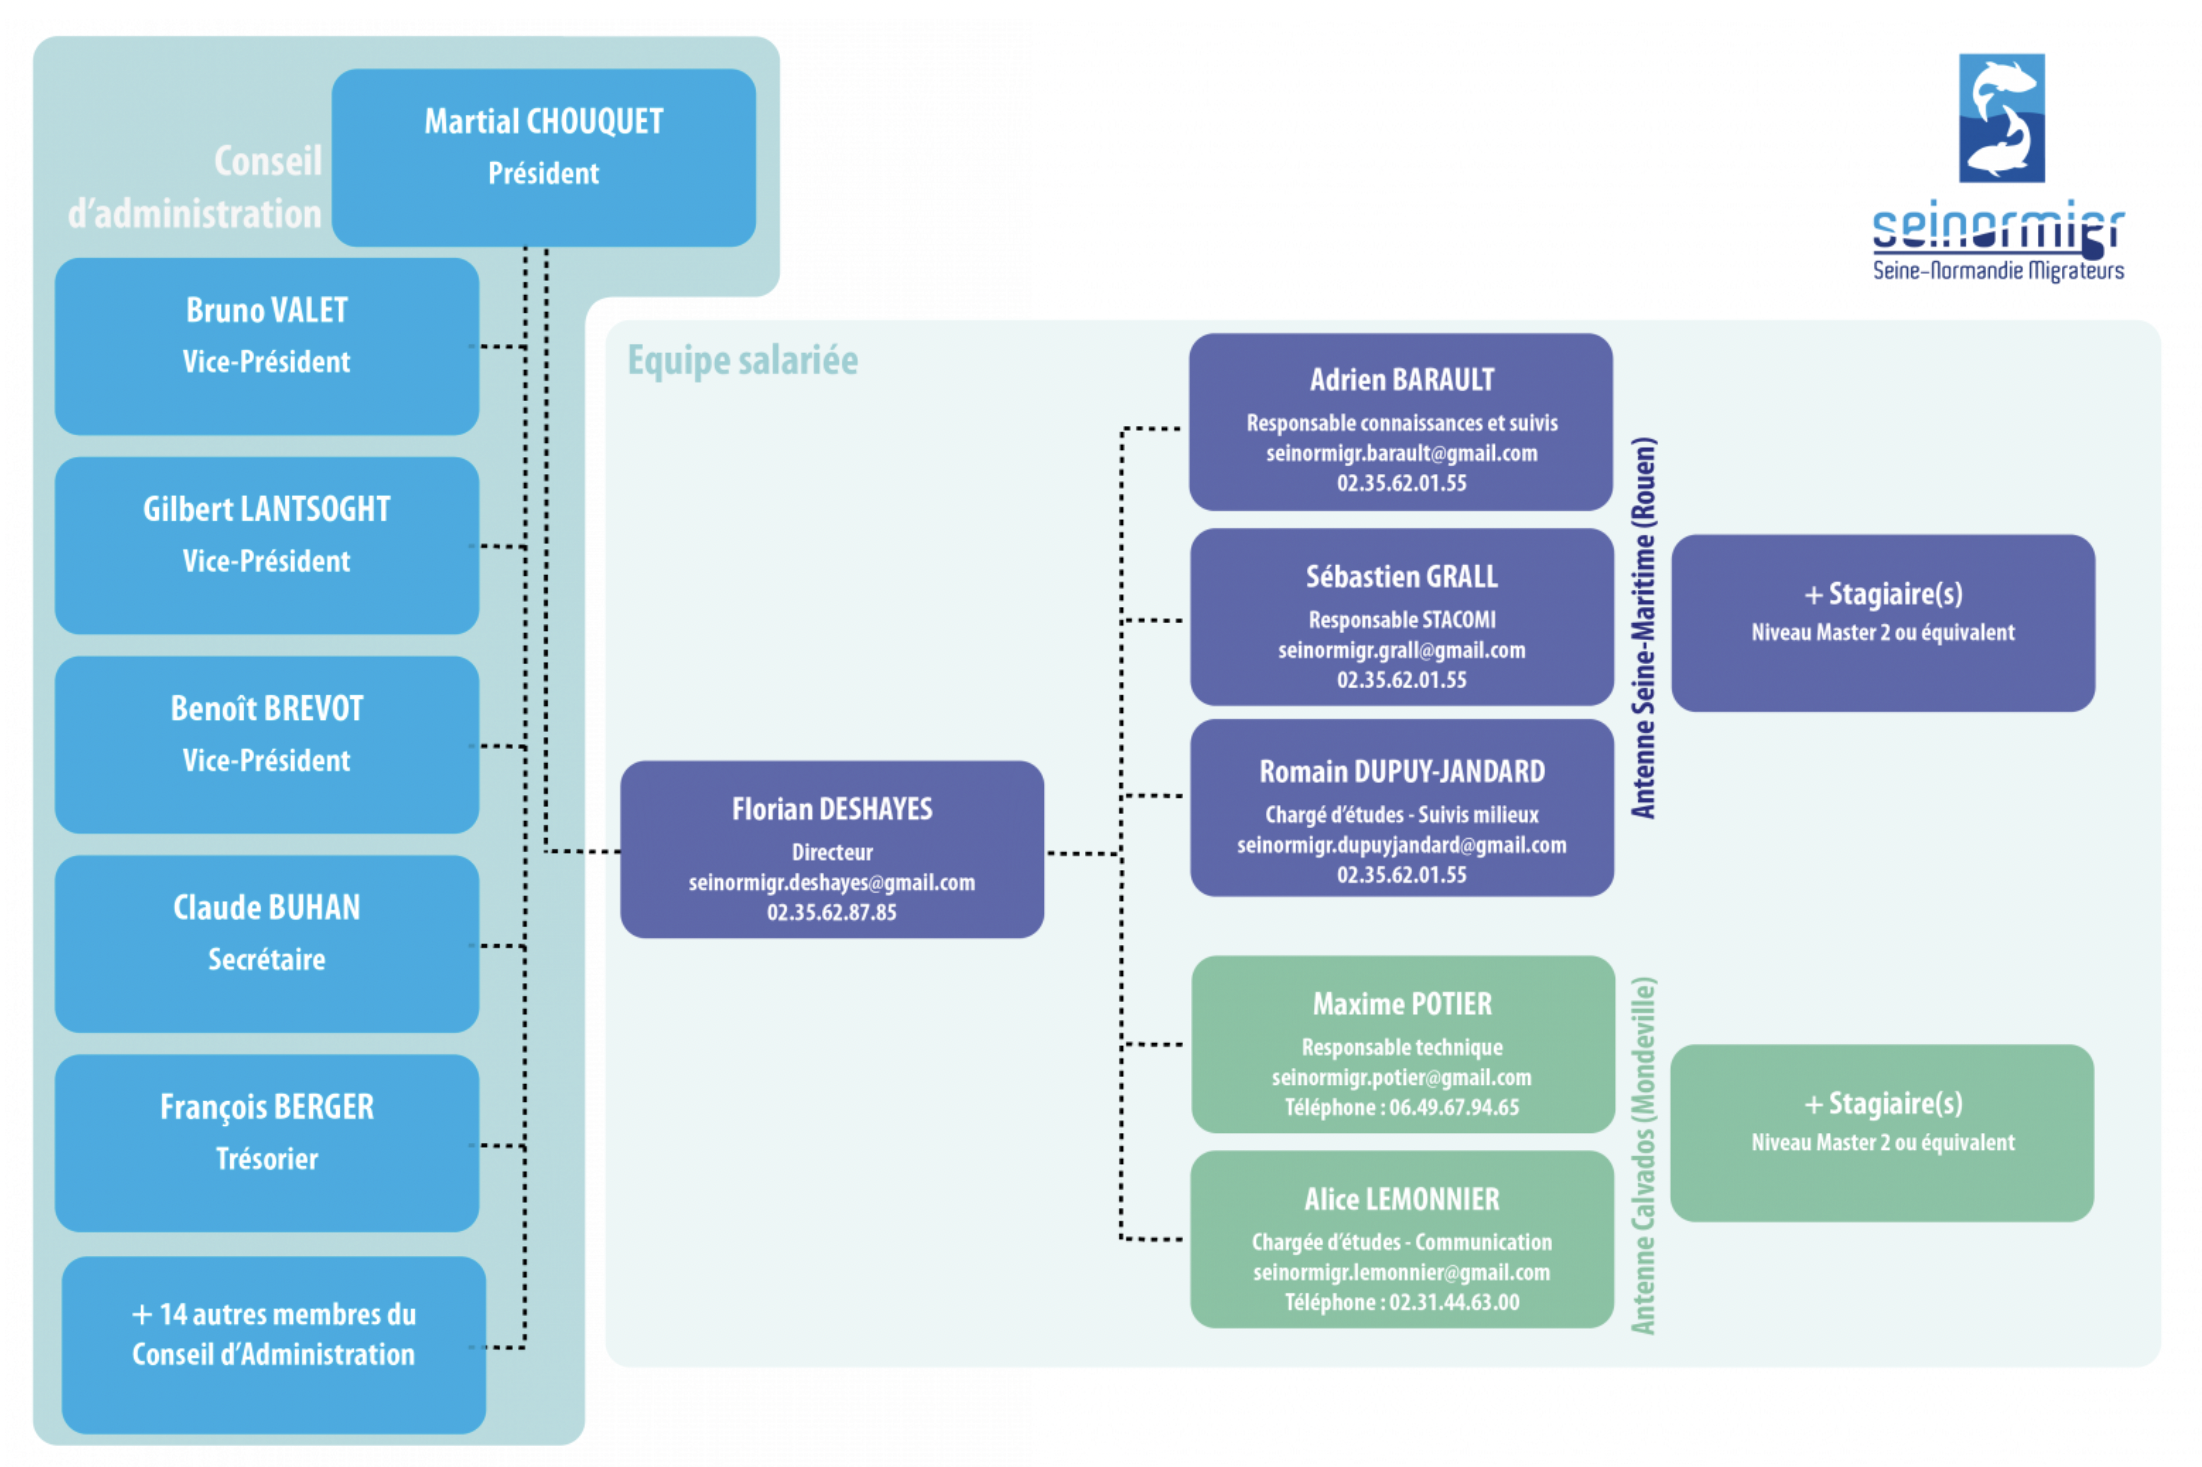
\includegraphics[width=\textwidth]{Organigramme_Seinormigr.png}
\caption{Organigramme de l'association Seinormigr}
\label{Organigramme_Seinormigr}
\end{figure}

-	Florian DESHAYES, Directeur (Rouen)

-	Maxime POTIER, Responsable technique (Mondeville)

-	Adrien BARAULT, Responsable - connaissances/suivis (Rouen)

-	Sébastien GRALL, Responsable - Stations de contrôle des migrations (Rouen)

-	Alice LEMONNIER, Chargée d'études – communication (Mondeville)

-	Romain DUPUY-JANDARD, Chargé d'étude - suivis milieux (Rouen)

\section{Introduction}

\subsection{Contexte historique de l’étude}

Les écosystèmes marins et dulcicoles jouent un rôle crucial pour l’humanité, fournissant des services essentiels (FAO 2020).
Cependant, au cours des dernières décennies, l'augmentation rapide des activités anthropiques, telles que l'urbanisation, l'industrialisation, et l'agriculture intensive, a entraîné une dégradation significative de ces environnements naturels (FAO 2020).
Les activités humaines constituent la 1ère cause érosion de la biodiversité mondiale (UICN).
En France, près de 25\% des poissons dulçaquicoles et amphihalins sont considérés à minima comme menacés (18 espèces sur 80) (UICN, 2019).
Il est estimé que près d’une espece d’eau douce sur trois est menacée d’extinction (WWF 2020).

L’anguille européenne est une des espèces qui a été extrêmement touchées par ces menaces \citep{dekker_climbing_2016}. Autrefois abondante dans les eaux européennes, jugée nuisible jusqu’en 1984, l’espèce représentait plus de 50\% de la biomasse piscicole de l’aval des systèmes fluviaux.
Ensuite, la population d'anguilles a drastiquement diminué depuis le milieu du XXème siècle. Initialement classée comme "vulnérable", elle est ensuite passée à "en danger", pour finalement aujourd’hui atteindre le statut "en danger critique d'extinction" selon l'Union internationale pour la conservation de la nature (UICN). Des études ont montré qu’aujourd’hui, selon les auteurs, le recrutement aurait diminué entre 90 et 99\% depuis 1960 \citep{feunteun_review_2003,baisez_outil_2005}.
L’anguille par son cycle de vie à la fois en eau de mer et en eau douce est confrontée à de nombreux phénomènes
qui sont à l’origine de ce déclin rapide : la dégradation des habitats, la pollution, le braconnage mais aussi les
changements climatiques notamment \citep{dekker_worldwide_2003}.
Face à ce déclin, la Commission Européenne, par le règlement (CE) n\degree 1100/2007, exige à chaque état membre l'élaboration d'un plan de gestion national (PGA), instauré en France depuis 2009.
Ce plan mis en place pour la conservation et la gestion durable de l'anguille européenne est décliné localement en unités de gestion (UGA) dans lesquelles des zones d'actions prioritaires (ZAP) sont déterminées.

Le bassin Seine-Normandie est un bassin jouant un rôle important dans la conservation de l’anguille car il est le bassin le plus important au niveau de la production d’anguille argentées mais aussi le second au niveau des anguilles jaunes  \citep{jouanin_eel_2012}.
Sur la Seine, l’évaluation du recrutement d’anguille se fait au niveau du barrage de Poses car il est le premier ouvrage rencontré depuis la mer. Le barrage se situe à 160 kilomètres de la mer et représente un passage obligatoire pour la faune piscicole souhaitant coloniser l’amont de la Seine.
Sur ce barrage, des dispositifs de franchissement ont été construits pour les anguilles (2014 en rive gauche et 2017 en rive droite). Cette construction s’est faite afin de répondre aux objectifs du plan de gestion anguille (PGA) en vigueur depuis 2009 sur le bassin Seine-Normandie.
Depuis 2014, l’association Seine-Normandie Migrateurs (SEINORMIGR) est chargée de réaliser chaque année le suivi de la migration anadrome des jeunes anguilles. Ce suivi a pour but d’évaluer le recrutement annuel des anguilles en Seine, de comparer les recrutements interannuels, d’évaluer la fonctionnalité des dispositifs de franchissement, d’identifier les facteurs environnementaux influençant la migration mais aussi de fournir un indice de recrutement pour le Comité de gestion des poissons migrateurs (COGEPOMI) qui coordonne les différentes actions pour la gestion et la protection des poissons migrateurs, afin d’élaborer le Plan de Gestion des Poissons Migrateurs (PLAGEPOMI), plan quinquennal de gestion des poissons migrateurs.

Ce rapport présente une synthèse bibliographique sur le sujet d’étude \og l’Anguille européenne \fg{} puis une mise en contexte de la présence d’Anguille européenne sur le bassin Seine Normandie. Ensuite, La partie \og matériels et méthodes \fg{} décrit les dispositifs de franchissement ainsi que les protocoles. Enfin, les résultats sont commentés puis discutés avant la conclusion et les perspectives.

\section{Synthèse bibliographique}

\subsection{Présentation du modèle d’étude : l’anguille européenne}

\subsubsection{Classification}

\textit{Anguilla Anguilla}ou anguille européenne, est un poisson téléostéen appartenant à l'ordre des Anguilliformes (comprenant 15 familles) et à la famille des Anguillidae.
Selon l’INPN, sa systématique est la suivante : Tableau \ref{tableau 1}


\begin{table}[h!]
\centering
\begin{tabular}{||c | c ||} 
 \hline\hline
 Embranchement & Chordata   \\ 
 Classe & Actinopterygii  \\
 Ordre & Anguilliformes  \\
 Famille & Anguillidae   \\
 Genre & \textit{Anguilla} \\
 Espèce & \textit{Anguilla}   \\ [1ex] 
 \hline
\end{tabular}
\caption{Classification de l'anguille européenne (INPN)}
\label{tableau 1}
\end{table}


\subsubsection{Morphologie }

Étant donné sa morphologie particulière, l’anguille européenne est aisément reconnaissable. Le corps de l’anguille est serpentiforme, constitué d’une partie antérieure cylindrique et d’une région caudale aplatie, est caractéristique de ce poisson (Figure \ref{Morpho}) \citep{dekker_worldwide_2003}. Au stade larvaire, les larves leptocéphales ne font que quelques millimètres (5 à 90) pour seulement quelques dixièmes de grammes. Tandis qu’au stade adulte les plus gros individus (les femelles) peuvent atteindre jusqu’à plus de 140 cm pour environ 6 kg \citep{tutman_new_2007}. Les mâles eux sont plus petits et dépassent rarement 45 cm. Un dimorphisme sexuel existe lié à la taille des individus \citep{brusle_biologie_2001}. La longévité de l’anguille est estimée à une quinzaine d’années bien qu’elle fluctue selon la zone géographique. L’anguille possède des nageoires pectorales bien développées derrière les branchies mais ne possède pas de nageoire pelvienne. Les dorsales, caudales et anales fusionnent pour former une longue nageoire unique allant de l’anus au milieu du dos \citep{hirschinger_donnees_2015}. \textit{Anguilla Anguilla}, porte une peau épaisse recouverte de petites écailles ovales (profondément incrustées dans le derme apparaissant à 15-20 cm) \citep{feunteun_commercially_2011}.  L’anguille ne peut pas sauter et possède une nage limitée mais la production d’un mucus abondant lui permet de se déplacer par reptation.

\begin{figure}[htpb]
\centering
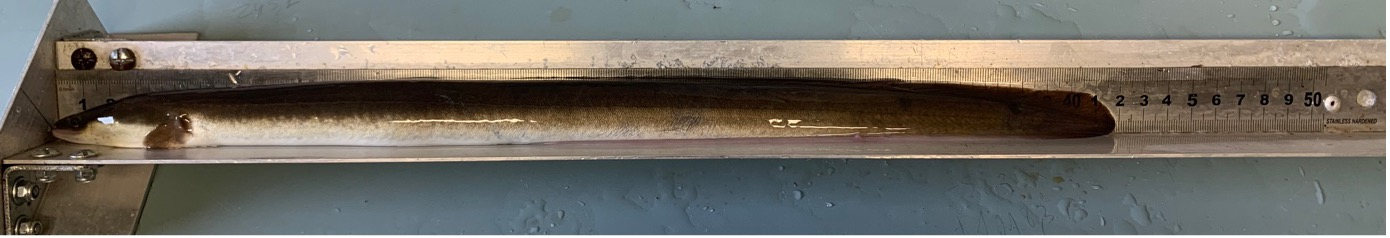
\includegraphics[width=\textwidth]{Morpho.jpg}
\caption{Anguille européenne "\textit{Anguilla Anguilla}". (Photo personnelle)}
\label{Morpho}
\end{figure}

\subsubsection{Régime alimentaire}


L’anguille est un prédateur opportuniste qui possède un régime alimentaire très varié, allant d’insectes, de larves aquatiques, de vers mais aussi de poissons. Son régime devient exclusivement piscivore à partir de 30-35 cm \citep{feunteun_commercially_2011}. Au début, les larves leptocéphales se nourrissent en mer d’organismes planctoniques pendant leur migration transatlantique \citep{riemann_qualitative_2010}. 
Sur le continent, elles deviennent omnivores et consomment notamment des algues, des bryozoaires, des annélides polychètes, des larves et des adultes d’insectes (diptères, trichoptères, éphéméroptères et odonates), des mollusques (moules et gastéropodes), des crustacés décapodes et des poissons \citep{pasquaud_determination_2010, jobling_eel_2004}. L’anguille est une proie pour de nombreux ardéidés \citep{feunteun_assessment_1994}.
Aussi, les flux énergétiques entre le milieu dulçaquicole et marin accordent à l’anguille une importance écologique non négligeable. On parle alors d’espèce clé, sa fluctuation en nombre amène différents effets sur d’autres espèces ou même l’écosystème \citep{willson_anadromous_1995}. Pour toutes ces raisons, elle doit être considérée comme une espèce parapluie, en protégeant l’anguille d’autres espèces le seront aussi \citep{baisez_outil_2005}.

\subsection{Aire de répartition}
	
L’anguille européenne est un poisson migrateur amphihalin thalassotoque \citep{adam_anguille_2008, brusle_anguille_1994, elie_migration_1994}, c’est- à-dire qu’au cours de sa vie, la reproduction se fait en mer tandis que la phase de croissance aura lieu dans les eaux côtières et douces continentales. Son aire de répartition est ainsi très vaste \citep{durif_migration_2003}. Les anguilles européennes sont distribuées le long de la côte ouest de l’Europe, au nord du continent africain, dans le bassin méditerranéen ainsi qu’en Islande (Figure \ref{Aire}). Cette distribution coïncide avec l’extrémité de la circulation anticyclonique des masses d’eaux de l’Atlantique Nord \citep{anthony_bases_2006}. Le site probable de ponte, en mer des Sargasses s’étend entre 23° et 30° Nord et entre 48° et 75° Ouest \citep{mccleave_reproductive_1987}. À la suite de l’éclosion des œufs les larves d’\textit{Anguilla Anguilla} se laissent porter par le Gulf Stream dans la moitié Nord de l’océan Atlantique. Pour la partie eau douce, la répartition de l’anguille européenne se limite aux obstacles qu’elle peut retrouver dans les cours d’eau \citep{adam_anguille_1997}. L’anguille est l’espèce ichtyologique colonisant la plus grande diversité d’habitats, disponibles depuis la mer, sur l’ensemble du territoire français \citep{laffaille_spatial_2003, laffaille_habitat_2004}. La population d’\textit{Anguilla Anguilla} est associée à un caractère panmictique du fait de la présence d’un seul stock se reproduisant en mer des Sargasses \citep{schmidt_ivbreeding_1922}. Cependant, des études plus récentes remettent en question cette panmixie en affirmant l’existence d’une diversité génétique au sein de la population. \citep{farrugio_etat_2011, pujolar_genetic_2007, daemen_analysis_2001}.

\begin{figure}[htpb]
\centering
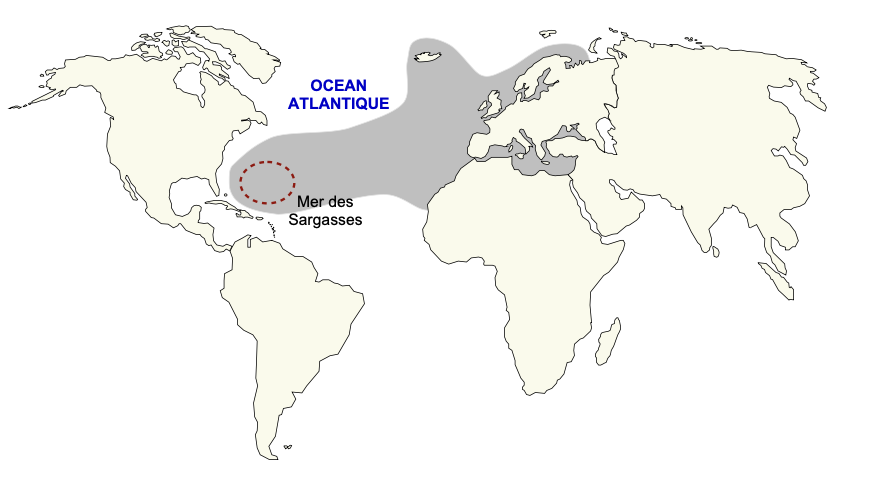
\includegraphics[width=\textwidth]{Aire}
\caption{Aire de répartition de l'anguille européenne. La zone de reproduction est représentée en rouge. (Imbert 2008)}
\label{Aire}
\end{figure}


\subsection{Cycle de vie}

Le cycle biologique de l’anguille européenne est assez complexe et présente encore quelques points méconnus. Au cours de sa vie l’anguille effectue deux migrations transocéaniques (anadrome et catadrome), une phase de croissance continentale (sédentarisation), deux métamorphoses et vraisemblablement, une unique reproduction (Figure \ref{Cycle}) \citep{anthony_bases_2006}. 

\begin{figure}[htpb]
\centering
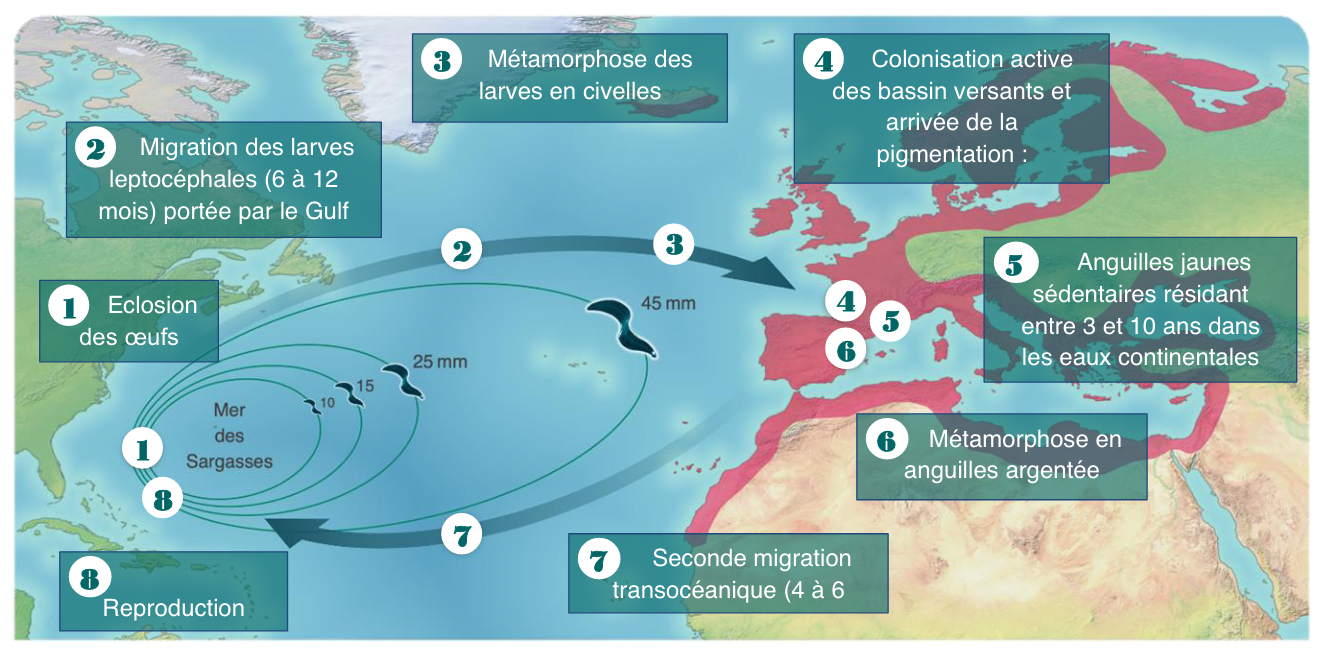
\includegraphics[width=\textwidth]{Cycle}
\caption{Répartition et cycle biologique de l'anguille européenne (Association MRM)}
\label{Cycle}
\end{figure}

\subsubsection{Larve leptocéphale}

La larve leptocéphale est le premier stade de l’espèce qui apparait à la suite de l’éclosion des œufs en mer des Sargasses, après la reproduction à des profondeurs comprises entre 200 et 400 mètres. La larve leptocéphale est translucide, en forme de feuille de saule est particulièrement adaptée à un mode de vie pélagique (Figure \ref{larve}) \citep{edeline_role_2005}. La larve dispose de glycosaminoglycanes (GAG) constituant une enveloppe corporelle très hydratée sous forme de composés hydrophiles. Ceux- ci maintiennent et hydratent le corps larvaire de l’individu. D’après \citep{bonhommeau_duration_2010} la migration des larves vers le continent européen dure environ 21 mois. Les larves effectuent des migrations nycthémérales restant entre 200 et 300 m de profondeur pour éviter les prédateurs la journée et remonte à 25 m de la surface la nuit pour se nourrir \citep{castonguay_vertical_1987}. A l’approche des côtes, les larves cessent de se nourrir \citep{edeline_role_2005} et commencent leur métamorphose en civelles \citep{hirschinger_donnees_2015}.

\begin{figure}[htpb]
\centering
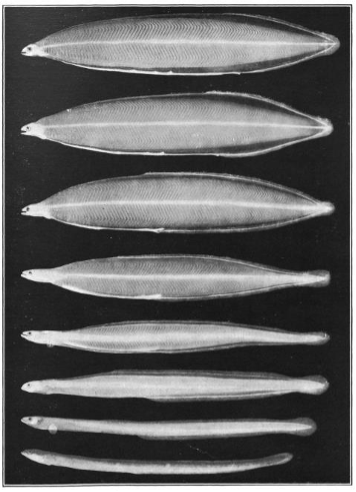
\includegraphics[width=0.4\textwidth]{larve}
\caption{Larve leptocéphale}
\label{larve}
\end{figure}

\subsubsection{Civelle}

Le stade civelle permet aux individus de coloniser le milieu continental \citep{edeline_role_2005}. La température de l’eau ainsi que la salinité conditionnent la vitesse de métamorphose \citep{laffaille_point_2005}. Les civelles ont une taille comprise en 60 et 80 mm (Figure \ref{civelle}) \citep{adam_anguille_2008}.  Elles colonisent les bassins versants en utilisant les courants de marée de flot \citep{hirschinger_donnees_2015}. Durant la colonisation des milieux continentaux le corps des civelles se pigmente progressivement \citep{prouzet_etude_2003} et l’alimentation s’arrête \citep{prouzet_historique_2002} . Le stade civelle dure environ 3 mois. La fin de la métamorphose est marquée par une pigmentation totale du corps dès lors la civelle devient une anguillette \citep{laffaille_role_2000}.

La remontée des civelles est conditionnée par divers facteurs : le crépuscule \citep{bardonnet_influence_2003, bardonnet_etude_2005}, la température de l’eau, avec une augmentation des captures à 20°C \citep{white_environmental_1997}, la marée montante \citep{bardonnet_influence_2003} et le cycle lunaire avec plus d’activité pendant la deuxième moitié du cycle \citep{todd_timing_1981}. 

\begin{figure}[htpb]
\centering
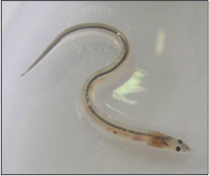
\includegraphics[width=0.5\textwidth]{civelle}
\caption{Civelle (SEINORMIGR))}
\label{civelle}
\end{figure}

\subsubsection{Anguille jaune }

Le stade anguille jaune apparait à la suite des anguillettes. La différence entre anguillettes et anguille jaune est que les anguillettes colonisent activement les cours d’eau alors que les anguilles jaunes marquent souvent la fin de la phase de migration anadrome. Ce stade anguilles jaunes correspond à une phase de croissance et de sédentarisation \citep{laffaille_point_2005}. Les individus sont pour la plupart sédentaire mais il n’est pas impossible que certains puissent maintenir de la mobilité \citep{laffaille_point_2005}. Le stade d’anguille jaune est caractérisé par une forte utilisation des ressources trophiques et une différenciation sexuelle de l’anguille. En effet, la spermatogénèse et l’ovogénèse sont simultanées, mais le développement du sexe mâle est notamment conditionné par un phénomène de densité dépendance : la production de mâles est majoritaire lorsque les densités de population et la disponibilité des ressources sont fortes \citep{passakas_karyological_1980}. L’âge de maturation est différent entre les mâles et les femelles, 3 à 9 ans pour les mâles (pour 20 à 150 g) contre 5 à 18 ans pour les femelles (pour 60 à 2100 g). Dès que les individus sont matures, ils s’argentent et la migration catadrome de dévalaison commence pour retourner vers la Mer des Sargasses (Figure \ref{ang_jaune_argent}) \citep{feunteun_commercially_2011,oliveira_life_1999}.

\begin{figure}[htpb]
\centering
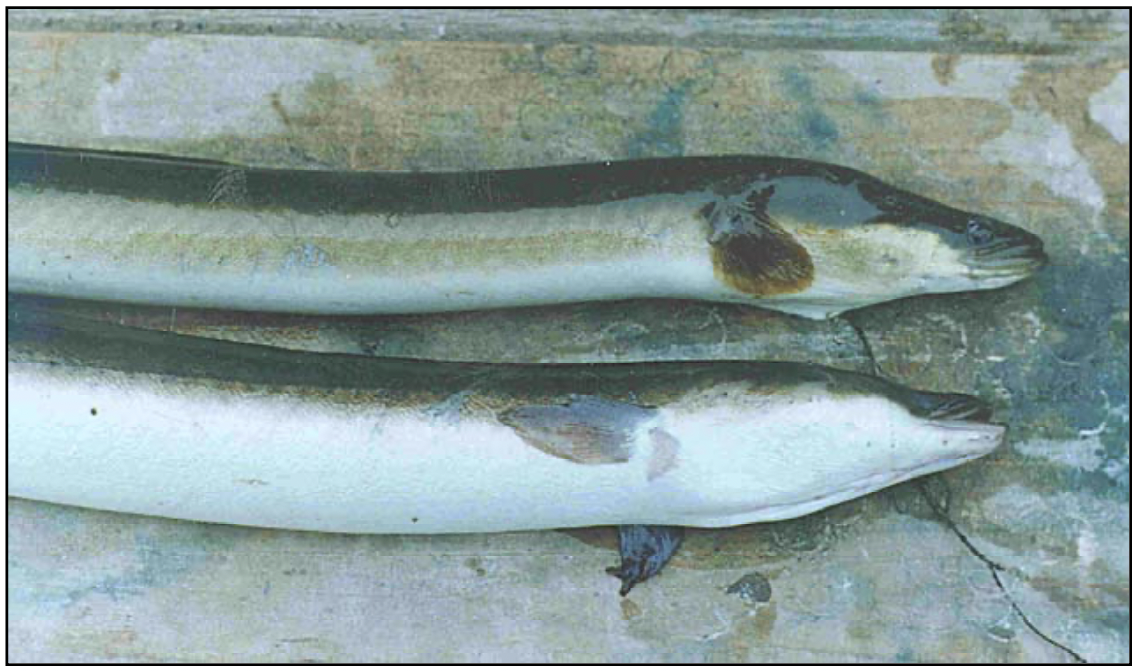
\includegraphics[width=\textwidth]{ang_jaune_argent}
\caption{Anguille jaune (haut) et anguille argenté (bas) (\citep{durif_migration_2003})}
\label{ang_jaune_argent}
\end{figure}

\subsubsection{Anguille argentée }


L’apparition d’argenture marque la fin de la période de croissance continentale mais aussi le début de différentes modifications morphologiques et physiologiques pour s’adapter à la vie en mer. Tout d’abord, il y a une pigmentation ombre sur le dos et blanche sur le ventre qui lui permet un camouflage marin. Un épaississement du derme et une surproduction de mucus \citep{saglio_structural_1988}.  Puis Les nageoires pectorales s’allongent \citep{durif_migration_2003}, le diamètre des yeux augmente et les photorécepteurs rétiniens se modifient \citep{adam_anguille_1997}. L’activité hormonale augmente \citep{lecomte-finiger_metamorphose_1990, pankhurst_structure_2006}. Enfin, il y a une augmentation du volume musculaire (de 5 à 13\%) et de l’activité hormonale \citep{lecomte-finiger_metamorphose_1990, pankhurst_structure_2006}. Une modification de la vessie gazeuse, assurant un maintien de la pression hydrostatique pour s’adapter aux profondeurs marines \citep{lecomte-finiger_metamorphose_1990} et une phase de répit alimentaire. L’argenture confère aux anguilles toutes les aptitudes morphologiques, physiologiques et énergétiques nécessaires pour effectuer leurs longues migrations transocéaniques vers la zone de reproduction et initie la maturation des organes géniteurs \citep{durif_durif_2009}. Ce comportement de dévalaison et d’argenture reste encore mal compris mais cela est associé à certains facteurs environnementaux comme la température, la photopériode et le cycle lunaire \citep{bruijs_silver_2009}. Plusieurs hypothèses sont données concernant l’élément influençant le déplacement des individus. Tout d’abord, la température et l’olfaction joue un rôle dans l’orientation des anguilles vers le lieu de ponte \citep{westin_orientation_1990}. Une autre piste plus probable est le champ magnétique car des études de \citep{nishi_magnetic_2004} et \citep{wu_neural_2012} ont montré une sensibilité des individus. Les anguilles sont des animaux sémelpares c’est à dire qu’ils meurent après la reproduction donc cet acte de reproduction est la dernière étape de leur vie. Cette reproduction s’effectuerait à environ 400 m de profondeur.

\subsection{Menaces }

Aujourd’hui l’anguille européenne est classée en danger critique d’extinction en France mais cela n’a pas toujours été le cas. Jusqu’en 1984, elle était encore classée nuisible (UICN). La population d’anguille européenne diminue drastiquement depuis le milieu des années 80 \citep{brusle_anguille_1994}. Les causes sont multiples, d’origine naturelle mais aussi et surtout anthropique liés à la colonisation de différents milieux lors de son cycle de vie.


\subsubsection{Pêche et braconnage }

Tous les stades continentaux de l’anguille sont exploités \citep{dekker_worldwide_2003}. Le stade civelle subit beaucoup de braconnage lié à la forte valeur économique du produit en Asie principalement. Le prix du kilo en Asie est environ 10 fois plus élevé qu’en France \citep{adam_anguille_2008}. La pêche amateure mais aussi professionnelle joue un rôle dans le déclin de l’espèce bien qu’elles ne sont pas considérées comme un phénomène principal \citep{prouzet_etude_2003}. 
Les recommandations du CIEM (Conseil international pour l’exploitation de la mer) de novembre 2021, valable pour les pêcheries 2022, préconisent une interdiction de la pêche à l’anguille. Bien que le repeuplement soit considéré comme une mesure de conservation par l’UE (article 7, 8°, du règlement 1100/2007), le CIEM observe que cette opération nécessite une récolte préalable des civelles. L’UE en autorisant la pêche commerciale est en contradiction avec le CIEM qui veut un arrêt de l’exploitation de cette espèce. 

\subsubsection{Parasitisme}

L’anguille est soumise à de nombreux parasites. Des parasites indigènes comme \textit{Acanthocephalus clavula} qui ne sont pas très impactant sur la vie de l’anguille avec des cas de mortalité très rares. Contrairement à cela, il y a des parasites introduits comme \textit{Anguillicola crassus}. Ce parasite a été introduit avec l’importation de l’anguille japonaise en Méditerranée. \textit{Anguillicola crassus} provoque une détérioration de vessie natatoire des individus ce qui va altérer l’organe \citep{kirk_effect_2000}. Le parasite provoque aussi des lésions de cette vessie natatoire qui va impacter les performances de nage, ce qui va demander plus d’énergie aux individus et donc compliquer fortement la migration trans océanique complète \citep{kirk_impact_2003}. 

 
\subsubsection{Prédation}

Tout comme la pêche, tous les stades de l’anguille sont soumis à la prédation commençant par des espèces de poissons marins durant la migration larvaire. Ensuite, lors de son arrivée sur le continent l’anguille va devenir la proie de nombreux poissons tels que le bar, le silure mais aussi de nombreux oiseaux comme les hérons ou le cormoran. L’anguille argentée lors de la migration de reproduction bien qu’elle soit beaucoup plus grosse peut être prédatés par des mammifères marins \citep{brusle_anguille_1994, carpentier_effects_2009}.

\subsubsection{Obstacles à la migration}

Le développement d’obstacles (barrages, déversoirs, buses, digues, ...) a considérablement augmenté entre les années 1950 et 1960 \citep{miller_did_2016}. La présence de nombreux obstacles sur les cours d’eau est une des principales causes de la diminution de la répartition et de l’abondance de l’anguille car l’accès à l’amont des cours d’eaux est difficile voire impossible \citep{adam_anguille_2008}. Tous les ouvrages vont retarder la migration des individus mais aussi provoquer une surdensité à l’aval des ouvrages pouvant provoquer compétition et augmentation de la prédation \citep{bevacqua_intra-specific_2011,drouineau_assessing_2014}. Durant la d’avalaison des anguilles argentées un autre problème se pose, les turbines des usines hydroélectriques. Les turbines créent un pourcentage de mortalité élevé pouvant atteindre presque 20\%. En cas de survie, le retard et l'augmentation des coûts énergétiques causée par le franchissement d'obstacles peuvent avoir des effets différés sur le succès de la migration et la fécondité \citep{van_ginneken_eel_2000}

\subsubsection{Perte et dégradation des habitats}

Les activités anthropiques provoquent une diminution de la surface et de la disponibilité des habitats favorables à l’anguille. Les principales causes sont la destruction des zones humides, le drainage mais aussi de nombreuse artificialisation des berges avec des endiguements par exemple \citep{basset_unifying_2013}. Il y a aussi la canalisation des rivières qui a pour effet de réduire leur largeur et de supprimer les berges latérales sauvages mais aussi les accès aux zones latérales (zones humides, marais…).

\subsubsection{Modifications hydro climatiques}

Les changements globaux entrainent une modification des températures mais aussi ont un impact sur les courants marins. De plus en plus d’études montrent que le recrutement des civelles est en lien avec des paramètres océaniques et atmosphériques \citep{bonhommeau_impact_2008, durif_influence_2010}. Une modification des courants marins du processus cyclique qu’est l’oscillation Nord-Atlantique (NAO) peut amener à une baisse de survie des larves leptocéphales lors de leur migration car cela va modifier l’intensité des courants dans l’océan \citep{durif_influence_2010}. En plus des phénomènes océaniques, la baisse des débits et des précipitations peut affecter les anguilles argentées car ce sont des déclencheurs importants de la migration d’avalaison \citep{bruijs_silver_2009}.

\subsubsection{Pollution}

L’anguille est fortement impactée par la pollution du fait de sa capacité à stocker des lipides mais aussi en raison de son niveau trophique, elle a un caractère bio-accumulateur \citep{brusle_anguille_1994,robinet_sublethal_2002}. De nombreux polluants sont retrouvés dans l’anguille comme les contaminants organiques, les métaux lourds et les pesticides \citep{bilau_probabilistic_2007,maes_catadromous_2005,couillard_correlation_2011}. L’impact des polluants sur l’anguille n’est souvent pas mortel mais se manifeste par des lésions tissulaires, des effets sur l’osmorégulation mais aussi des perturbations hormonales \citep{couillard_correlation_2011}. Cela peut provoquer des déclenchements précoces de migration alors que l’anguille ne possède pas de réserve énergétique et à contrario cela va pousser les anguilles à utiliser leur énergie pour des mécanismes de détoxication.


\subsection{Intérêt de l’anguille européenne }

\subsubsection{Écologique }


Sur le plan écologique, son caractère bio-accumulateur ou biointégrateur associé à sa capacité à coloniser tous les milieux aquatiques, font de l’anguille une espèce à fort intérêt dans l’expertise de la qualité d’un milieu \citep{laffaille_role_2000}. L’anguille européenne est même caractérisée d’espèce parapluie ce qui rendrait sa gestion profitable à l'ensemble des organismes cohabitants. La présence d’anguille ainsi que l’abondance renseignent sur le bon fonctionnement d’un écosystème et indique une certaine connectivité avec d’autres habitats (marais, annexes hydrauliques, plaines d’inondation...).


\subsubsection{Économique }

Sur le plan économique, l’anguille possède une très forte valeur marchande et est exploitée et commercialisée \citep{elie_migration_1994}.  En France, environ 6000 tonnes d’anguilles sont pêchées et déclarées chaque année \citep{baisez_outil_2005}. Le stade le plus exploité est la civelle,exporté illégalement vers l’Asie de l’Est (500 tonnes dans les années 2000). Pour le prix, les pêcheries européennes représentent un chiffre d'affaires estimé à 180 millions d'euro\citep{laffaille_role_2000}. L'anguille suscite donc un fort intérêt au niveau scientifique, de la gestion et conservation mais aussi aux pêches professionnelles.


\subsection{Mesures de conservation}

Le stock d’aguille européenne ne cesse de diminuer depuis les années 80. Cette constatation se fait sur le recrutement des civelles (baisse de 8\% par an depuis 1980) mais également sur le stock d’anguille installé dans les cours d’eau continentale (baisse de 3,4\% par an depuis 1983). Face à ce déclin, un Plan National de Gestion de l'Anguille (PGA) a été mis en place en 2009 pour une durée de trois ans renouvelables (Figure \ref{PGA}). Le PGA est composé d’un volet national, garantissant un cadre de travail homogène, et d’un volet local, permettant d’adapter le plan aux caractéristiques de chaque territoire. La France est ainsi divisée en neuf unités de gestion de l’anguille (UGA), dont celle de Seine-Normandie. (DRIEE Ile-de-France, 2016). 

Du point de vue du l’UGA Seine-Normandie, le Plan de gestion des poissons migrateurs du territoire Seine-Normandie a été renouvelé et couvre la période 2022-2027. Il s’agit d’étoffer les actions préexistantes et d’en développer de nouvelles sur le territoire, par exemple :

- La réalisation des campagnes de terrain, concentrées sur les Indices d’Abondance anguilles et saumons, via de nombreuses opérations de pêches électriques sur des fleuves côtiers ou sur le bassin de la Seine. Ces inventaires renseignent sur l’état des populations à l’échelle des bassins suivis. 

- Les dénombrements en continu au niveau des stations de contrôles, des migrateurs qui s’engagent dans les hydrosystèmes. 

- Le suivi des anguilles s’engageant sur l’axe Seine au niveau du barrage de Poses sur les deux rives. 

- Le déploiement d’un réseau de suivi de la thermie des cours d’eau, paramètre particulièrement important dans le développement et la répartition des migrateurs. 

\begin{figure}[htpb]
\centering
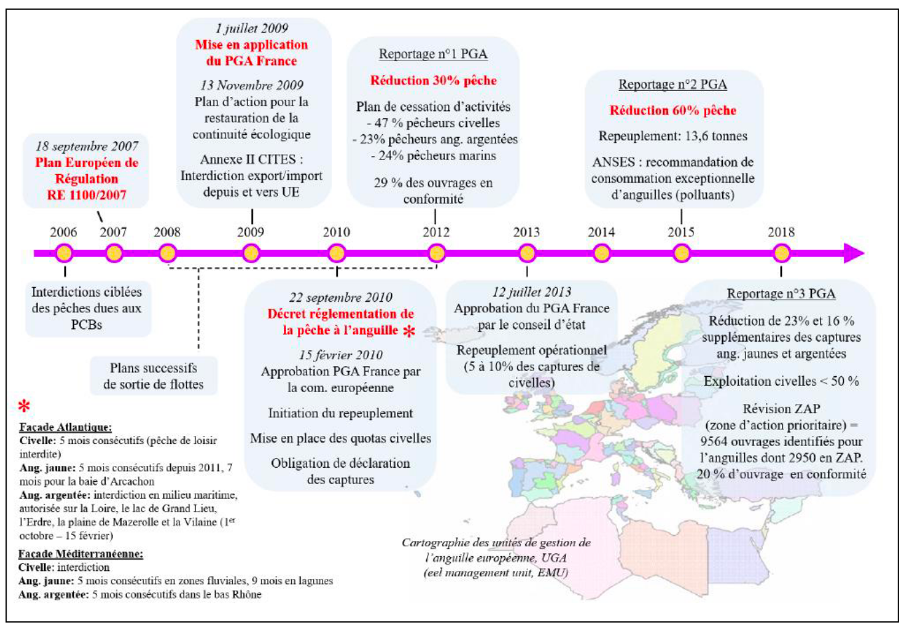
\includegraphics[width=\textwidth]{PGA}
\caption{Chronologie des plans de gestion de l’anguille européenne en place en France métropolitaine (GIPSA 2023)}
\label{PGA}
\end{figure}

\section{Contexte}

\subsection{Bassin Seine Normandie}


Le bassin Seine Normandie s’étend sur 6 régions, 28 départements et 8 138 communes pour une superficie de 95 000 km2 ce qui représente 18\% du territoire national et une population d’environ 18,3 millions d’habitants (Figure \ref{Bassin}). Il est constitué de la Seine mais aussi de ses affluents (l’Oise, la Marne, l’Yonne), et des cours d’eau côtiers normands (la Bresle, l’Arques, la Sélune, la Vire) (Agence de l’eau Seine Normandie). Ce bassin représente un total de 55 000 km de cours d’eau sur 18 bassins versants dont le principal est celui de la Seine (82,5\% du bassin). La Seine est l’un des plus grands fleuves de France avec une longueur de 770 km. La Seine prend sa source à Source-Seine (Côte d’Or) dans la région Bourgogne Franche Comté et se jette en Normandie entre Le Havre et Honfleur (Agence de l’eau Seine Normandie).

\begin{figure}[htpb]
\centering
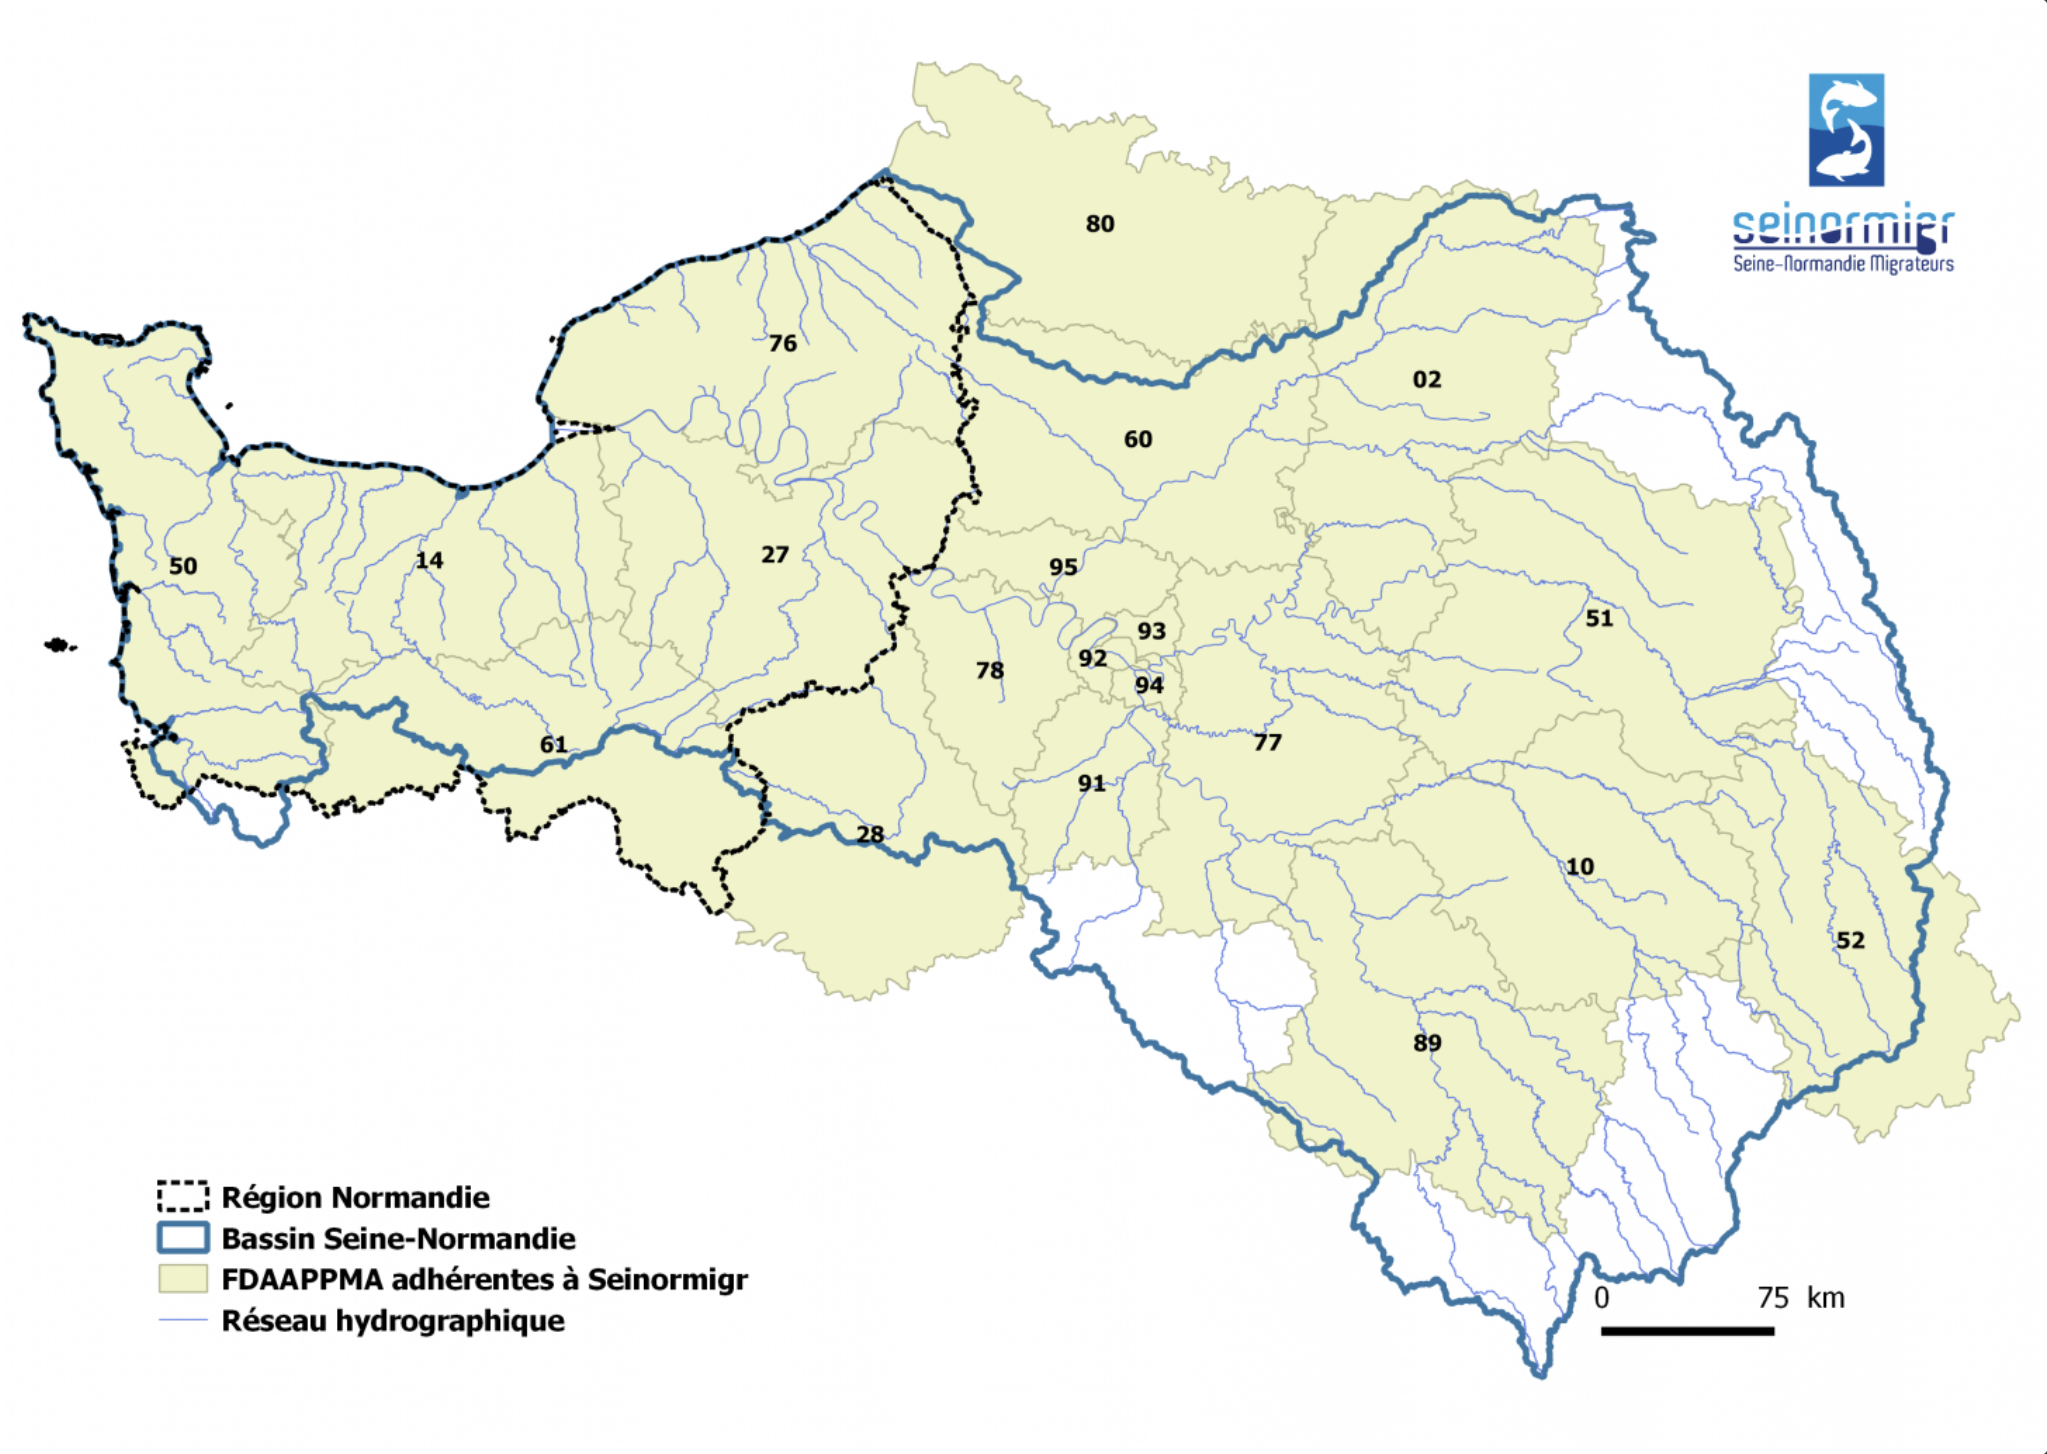
\includegraphics[width=0.5\textwidth]{Bassin}
\caption{Carte représentant le bassin versant de la Seine (SEINORMIGR).}
\label{Bassin}
\end{figure}

Concernant la qualité des eaux, la Seine est considérée comme l’un des cours d’eau les plus pollués. Cette région connait un fort transport fluvial et de nombreux aménagements ont été réalisés pour répondre à différents besoins croissants liés à l’augmentation démographique \citep{thieu_nutrient_2009}. En 1970, la Seine avait une zone anoxique de 100 km en aval de Paris, les animaux aquatiques aérobies, poissons y compris, ne pouvaient pas y vivre (DRIEE, 2016). Pour exemple, il existe 32 espèces piscicoles recensées au niveau de ce cours d’eau contre seulement 3 dans les années 1970 \citep{rocher_evolution_2017}. Des études ont montré des résultats encourageants entre 2013 et 2019 avec une augmentation de 38\%  à 41\% des masses d'eau en bon ou très bon état (Figure \ref{Qualité_eau}).


\begin{figure}[htpb]
\centering
\includegraphics[width=0.5\textwidth]{Qualité_eau}
\caption{État écologique des cours d’eau bassin Seine-Normandie (AESN/DRIEE, EDL 2019)}
\label{Qualité_eau}
\end{figure}

Au niveau des habitats, ils sont affectés par diverses modifications comme la chenalisation, la destruction de zone humide et la construction d’ouvrages. D’après l’Agence de l’eau en 2022, environ 1 500 km de cours d’eau sont devenus accessibles. Cependant, des projections d’ici 2027 ont montré que si aucune mesure n’est prise il pourrait avoir une diminution des masses d’eau en bon ou très bon état écologique. Le Schéma Directeur d'Aménagement et de Gestion des Eaux (SDAGE) 2022-2027, en vigueur, fixe la stratégie pour l'atteinte du bon état des milieux aquatiques en 2027.

\subsection{Sites d’études : Poses – Amfreville-sous-les-Monts}

\subsubsection{Le barrage}


Le barrage de Poses a été construit entre les années 1878 et 1885 entre les communes de Poses et d’Amfreville-sous-les-Monts dans le département de l’Eure. Plus souvent appelé le barrage de Poses, il a été construit en premier lieu pour la navigation. En 1991, une usine hydroélectrique a été rajoutée du côté de la rive gauche. Ce barrage est situé à 160 km de l’estuaire est le premier obstacle rencontré et subit encore à l’aval le phénomène de marée. Sur ce barrage 3 infrastructures se différencient avec l’écluse et les systèmes de vannages en rive droite et l’usine hydroélectrique en rive gauche (Figure \ref{Barrage}). 


\begin{figure}[htpb]
\centering
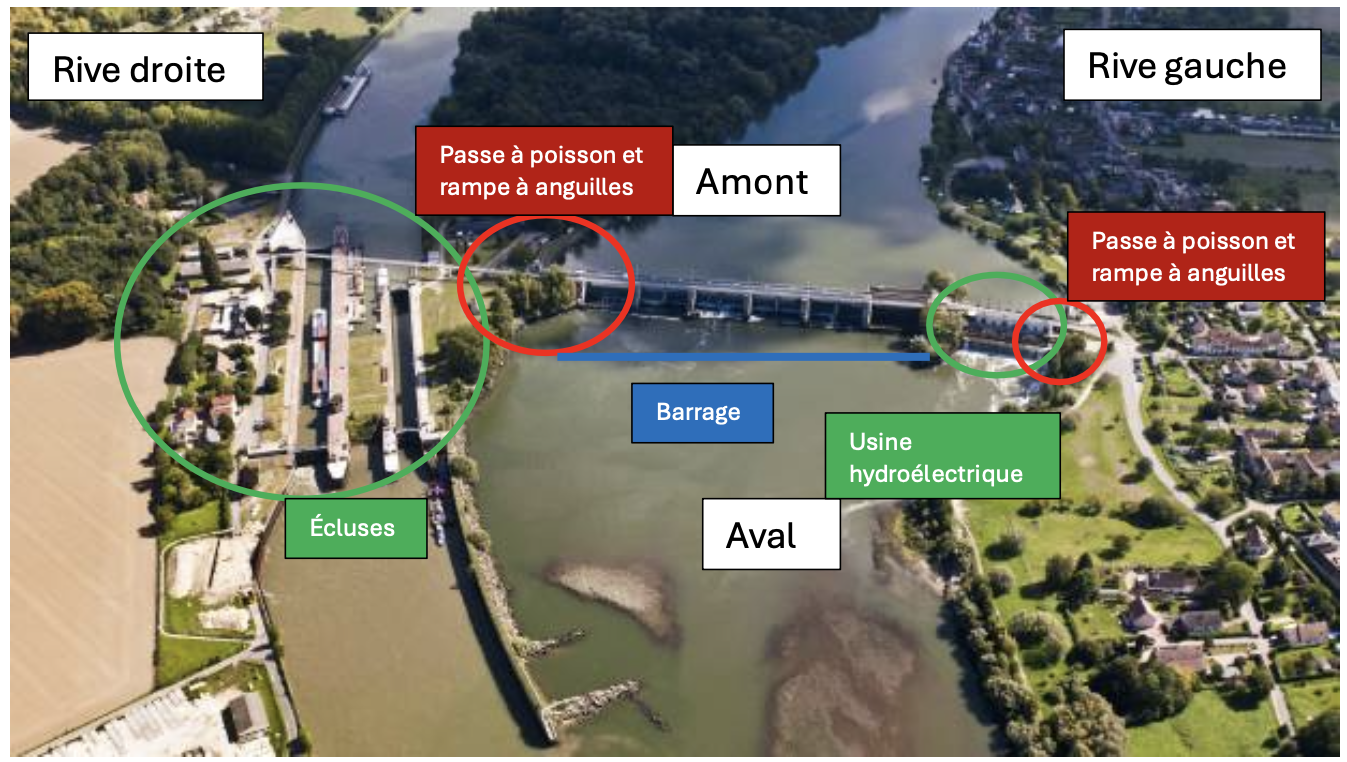
\includegraphics[width=\textwidth]{Barrage}
\caption{Présentation des infrastructures du barrage de Poses – Amfreville-sous-les-Monts}
\label{Barrage}
\end{figure}

\subsubsection{Les passes à poissons et le vidéo comptage}


La première passe à poissons a été construite en 1991 (rive gauche) pour permettre aux poissons migrateurs de franchir cet obstacle. La passe comporte 23 bassins successifs pour un total de 86 mètres ainsi que by-pass permettant le contournement de l’usine hydroélectrique pour la dévalaison. Par la suite, cette passe à poisson a été équipée en 2008 d’une chambre d’observation dans laquelle un système de vidéo-comptage a été mis en place permettant de connaître les espèces empruntant la passe. Seinormigr assure depuis 2020 le dépouillement des séquences vidéo.

Une seconde passe à poisson ainsi qu’un système de vidéo-comptage a été construit en 2017 en rive droite pour complémenter la passe à poissons en rive gauche pour le franchissement du barrage des poissons migrateurs. Cette passe à poissons comporte 28 bassins et le système de vidéo-comptage comporte deux couloirs d’observation tous les deux indépendants. Seinormigr assure ici aussi le dépouillement des séquences vidéo (Figure \ref{RD}),(Figure \ref{RG}).

\subsubsection{Les rampes à anguilles }

Des rampes à anguilles ont aussi été construites en parallèle des passes à poissons pour permettre aux anguilles de poursuivre leur migration car les anguilles ne sont pas de bonnes nageuses et les passes à poissons ne sont pas adaptées pour elles. Les installations ont eu lieu en 2013 pour la rive gauche et 2017 pour la rive droite.

\begin{figure}[htpb]
\centering
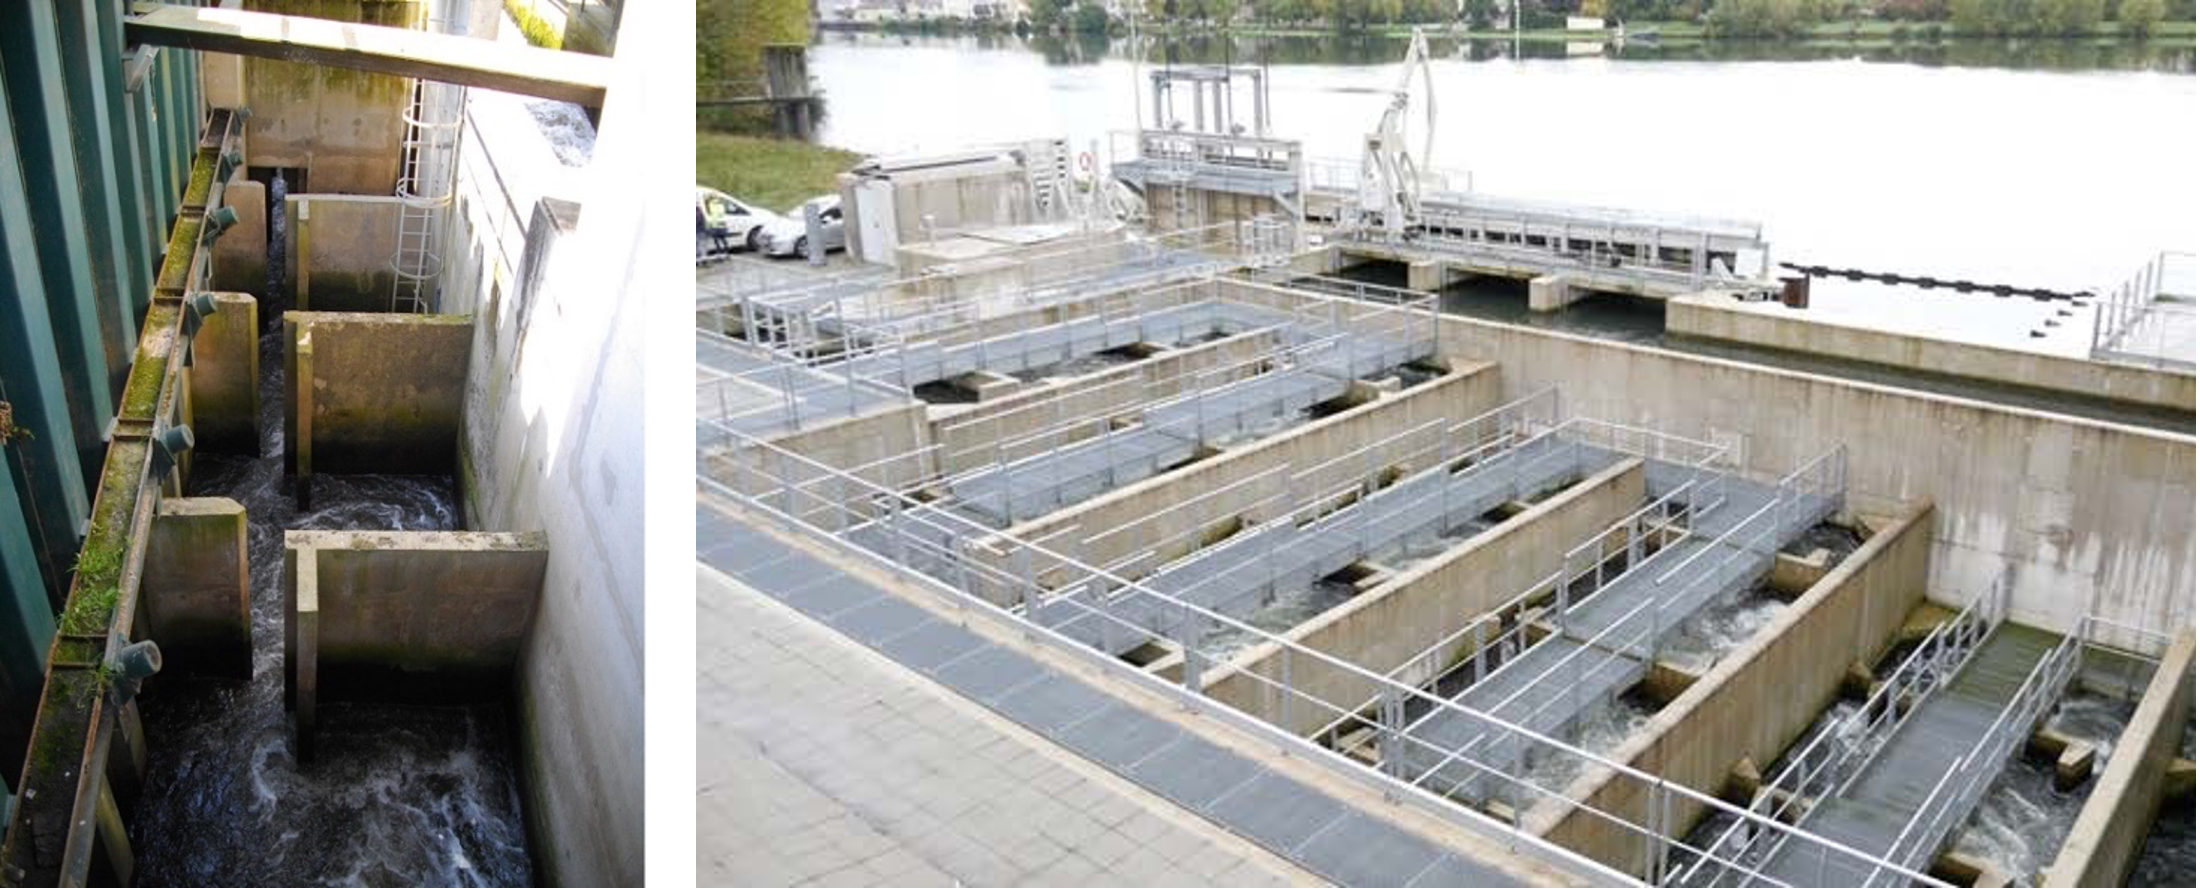
\includegraphics[width=\textwidth]{RD}
\caption{Passes à poissons (Rive gauche photo de gauche, Rive droite photo de droite). (SEINORMIGR)}
\label{RD}
\end{figure}

\begin{figure}[htpb]
\centering
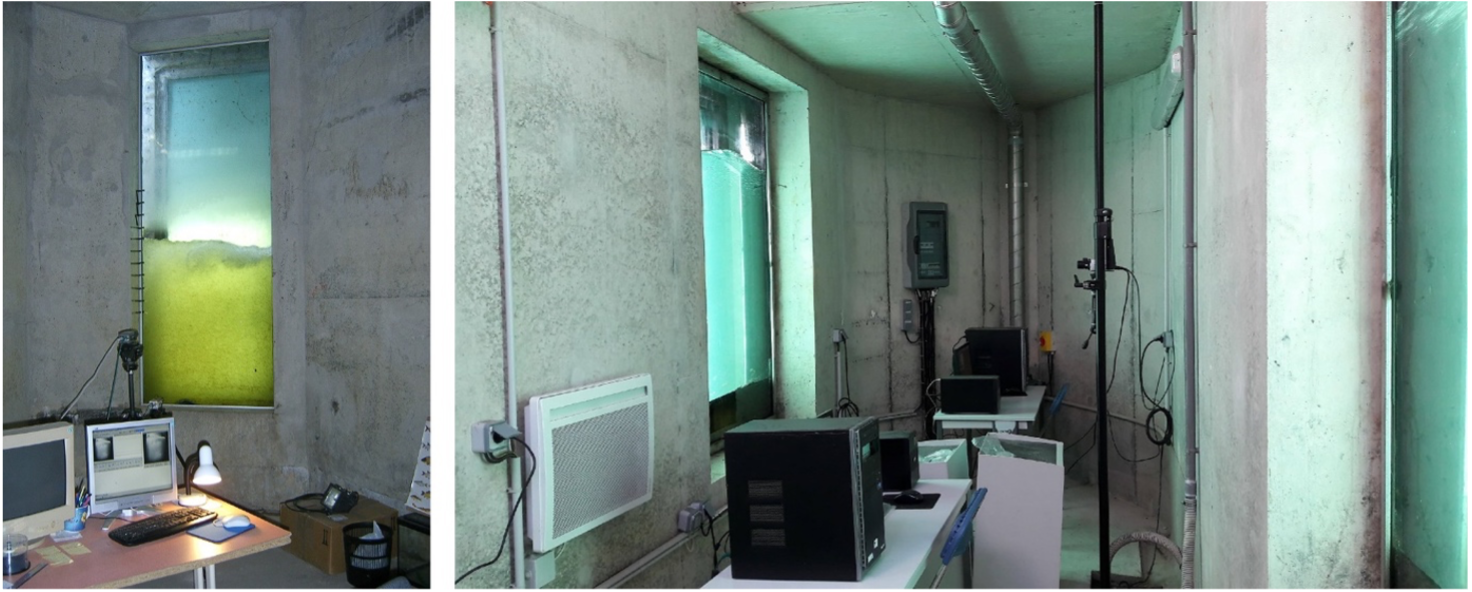
\includegraphics[width=\textwidth]{RG}
\caption{Système de vidéo-comptage (Rive gauche photo de gauche, Rive droite photo de droite). (SEINORMIGR)}
\label{RG}
\end{figure}

\section{Matériels et méthodes}

\subsection{Les pièges actifs }

Les jeunes anguilles contrairement aux anguilles adultes et aux autres espèces de poissons migrateurs ne peuvent pas utiliser les passes à fentes verticales du barrage. Cette exception est liée aux faibles capacités de nage des individus (nage et vitesse de pointe n’allant que de 0,3 à 0.9 m/s) \citep{cowx_enhancing_2003, crivelli_languille_1998}. Des passes à anguilles sont mises en place pour permettre aux individus de continuer leurs migrations. Les rampes sont inclinées et une fine couche d’eau doit être présentes sur la rampe pour permettre aux anguilles de monter avec leur capacité de reptation. Les rampes spécifiques anguilles (types brosses), se montrent particulièrement adaptées pour les jeunes stades et sont donc employées sur le site d’étude. 

\subsubsection{Rive gauche}

La rampe a été ajoutée en 2013. D’une longueur totale de 61 m, elle se décompose en 3 parties distinctes (Figure \ref{RG2}):

Première partie l’aval : Cela commence avec une 1ère rampe dont la base est immergée en permanence, cela permet l’entrée des individus dans le dispositif (photo 1). Ensuite, deux autres rampes sont à la suite. Elles sont toutes les deux inclinées à 45° et séparées par un bassin de repos (photo 2). Ces dispositifs sont situés en aval de la centrale hydroélectrique et débouchent sur une cuve connectée à un canal de liaison (photo 3). 

Seconde partie le canal de liaison : Avec une légère inclinaison négative de 2°, le canal (tube PVC), d’une longueur de 56 m, permet une montaison des anguilles (photo 4-5). Il se déverse dans un collecteur, au pied d’une nouvelle rampe (photo 6). 

Dernière partie l’amont : Cette dernière rampe (inclinée à 35°) dirige les anguilles vers le dispositif de piégeage (photo 7). Il s’agit d’une cuve équipé d’un filet pour empêcher les fuites mais aussi faciliter la récupération des individus où tombent les anguilles (photo 8). 

\begin{figure}[htpb]
\centering
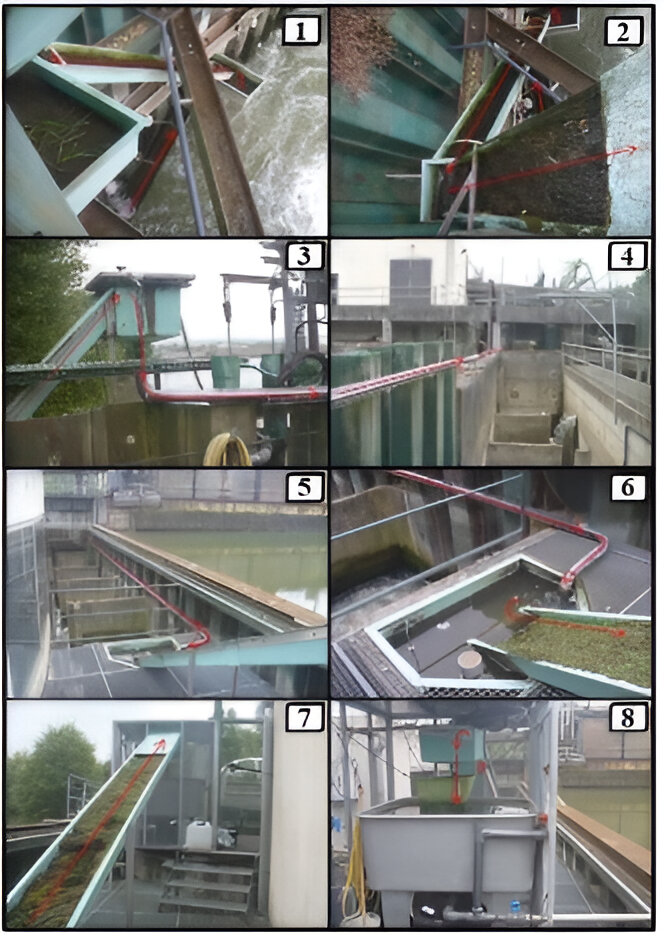
\includegraphics[width=0.4\textwidth]{RG2}
\caption{Dispositif de franchissement anguille en rive gauche sur le barrage de Poses. Les flèches rouges indiquent le trajet des individus}
\label{RG2}
\end{figure}

\subsubsection{Rive droite }

Cette rampe a été construite en 2017 en même temps que la passe à poissons et elle est plus adaptée que le dispositif en rive gauche. D’une longueur totale de 100 m, elle se décompose elle aussi en 3 parties distinctes (Figure \ref{RD2}) :

Première partie l’aval : Tout d’abord, une 1ère rampe est succédée d’un bassin de repos puis d’une nouvelle rampe (photo 1). Ces rampes sont inclinées à 45° et sont alimentées par surverse via un canal en amont (photo 2).

Seconde partie le canal de liaison : Le canal (long de 80m) oriente les anguilles vers le dispositif de piégeage (photo 3 à 5). 

Dernière partie l’amont :  Enfin, les anguilles empruntent une dernière rampe (inclinée à 45°), pour finir dans la cuve de piégeage en attendant leurs manipulations (photo 6).

\begin{figure}[htpb]
\centering
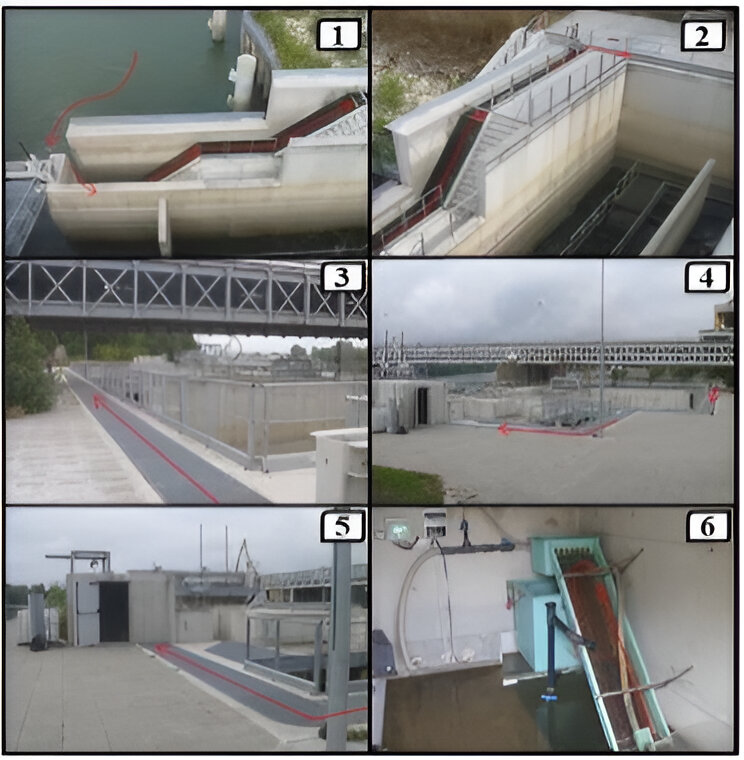
\includegraphics[width=0.5\textwidth]{RD2}
\caption{Dispositif de franchissement anguille en rive droite sur le barrage de Poses. Les flèches rouges indiquent le trajet des individus}
\label{RD2}
\end{figure}

\subsection{Protocole de suivi }

\subsubsection{Suivi des anguilles }

A Poses, les premières observations ont lieu début avril (lorsque la température de l’eau dépasse les 14 °C). Les individus observés durant cette période sont des anguillettes en reprise de migration, en attendant l’arrivée des civelles. Cette année, le suivi a été mis en place le 2 avril et sera poursuivi jusqu’en octobre. 
Les pièges sont relevés trois fois / semaine en période creuse et une relève est faite tous les jours lorsque la migration s’intensifie. Une intervention les week-ends ou jours fériés est nécessaire en cas de fort pic de migration pour éviter des mortalités dues à une surdensité d’individus dans la cuve de piégeage. Une demi-journée à deux opérateurs est généralement nécessaire pour une opération de suivi.

\subsubsection{Entretien des pièges}

Lors de chaque relève, les pièges sont nettoyés et leur fonctionnement est vérifié. De manière générale, les points de contrôle (sensiblement différents selon la rive) sont listés dans le tableau ci-dessous Tableau \ref{tableau 2}. 


\begin{table}[h!]
\centering
\begin{tabular}{|c|c|c|} 
\hline
 Contrôle &   &  \\ [0.5ex] 
 \hline
 Objet & Rive gauche  & Rive droite \\ 
 \hline
 Fonctionnement de l’armoire électrique et des pompes  & oui  & oui \\
 Alimentation en eau des rampes et débit d’eau dans les répartiteurs & oui & oui \\
 Débits dans le canal de liaison et éventuels débordements du 2ème collecteur & oui &  non \\
 \hline
 Nettoyage &   & \\ [0.5ex] 
 \hline
 Objet & Rive gauche & Rive droite \\
 \hline
 Enlèvement des fines et débris dans le vivier (cuve), le filet et le répartiteur  & oui  & oui \\
 Enlèvement des fines et débris dans le 2ème collecteur et autour de la crépine  & oui &  non \\ [1ex] 
 \hline
\end{tabular}
\caption{Liste des Operations d'entretien des pièges à anguilles du barraghe de Poses}
\label{tableau 2}
\end{table}

\subsubsection{Obtention des données biométriques}

Tout d’abord, selon le nombre d’anguilles présentes dans la cuve une partie ou la totalité des individus sont anesthésies dans une solution d’eugénol (huile essentielle de clous de girofle) diluée dans l’eau. Cela permet de faciliter les manipulations des anguilles. Ensuite, les mesures biométriques sont effectuées dans l’ordre suivant : 
-	Longueur totale (Lt) en mm, à l'aide d’un ichtyomètre (± 1 mm). 
-	Identification d’éventuelles anomalies anatomo-morphologiques, d’après la grille de codification établie par \citep{elie_sante_2014}. 
-	 Poids (P) en g, à l'aide d’une balance électronique (± 0,1 g). 
Pour le réveil, d’une durée de quelques minutes, les anguilles sont conservées dans des seaux d’eau. Elles sont ensuite relâchées, en rive droite, en amont du barrage pour que les individus puissent poursuivre leur montaison. Les effectifs capturés varient d’une relevé à une autre. Aussi, un protocole de dénombrement est établi (Figure \ref{Protocole}). 

\begin{figure}[htpb]
\centering
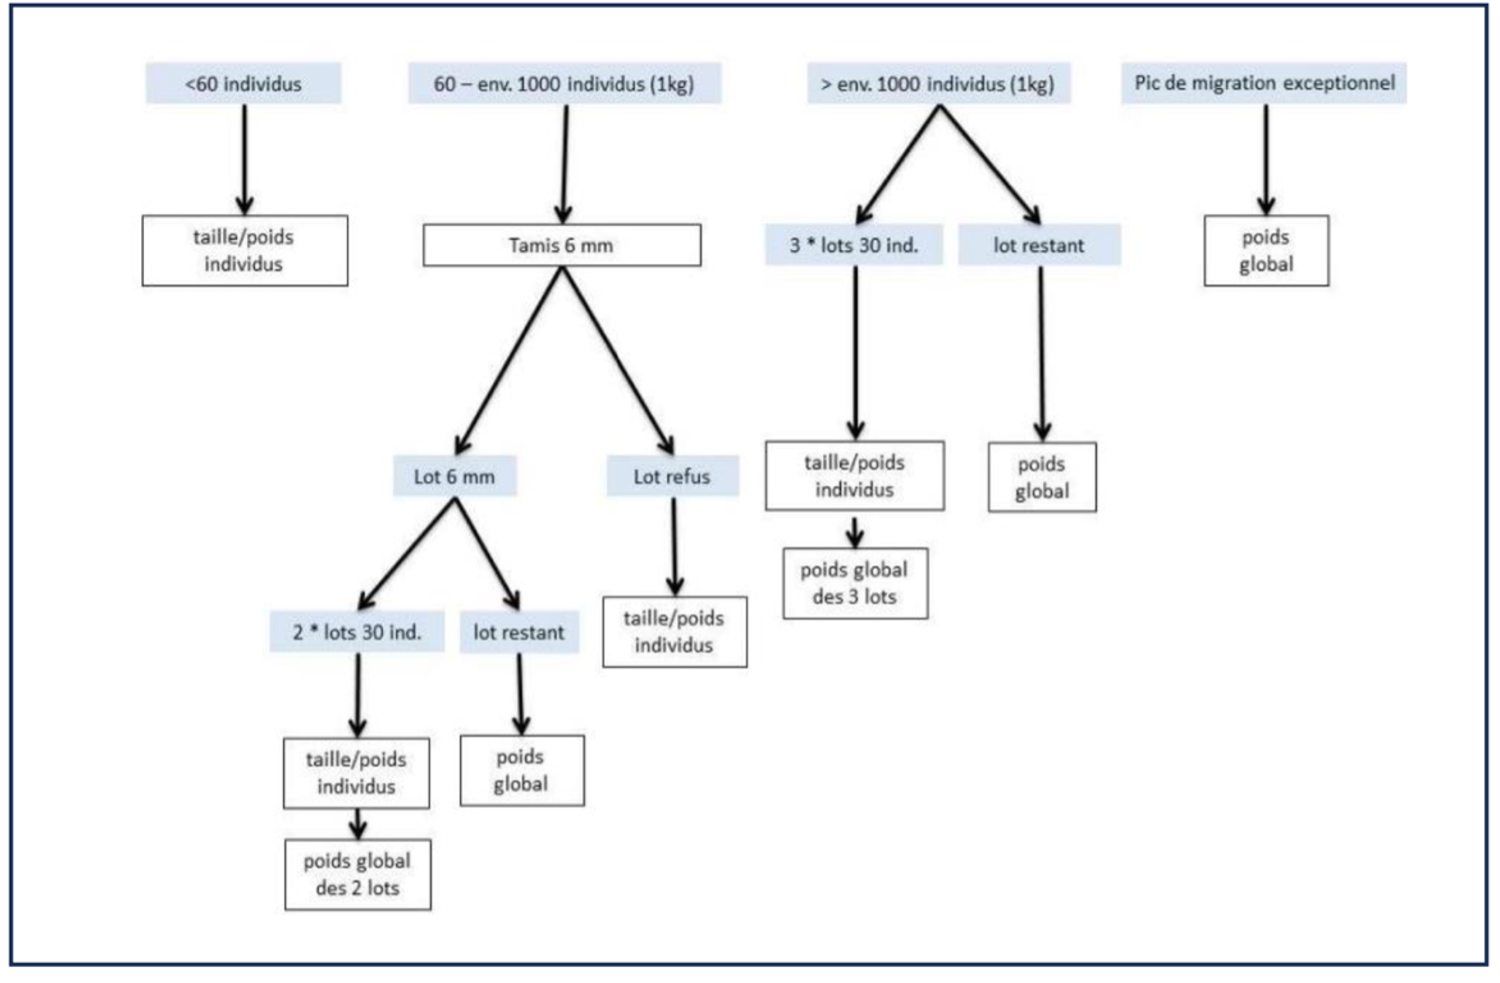
\includegraphics[width=0.5\textwidth]{Protocole}
\caption{Protocole de dénombrement des anguilles (SEINORMIGR)}
\label{Protocole}
\end{figure}


\subsubsection{Saisie et bancarisation des données}

Sur le terrain, des carnets (un pour chaque rive) sont utilisés pour saisir les données. Pour chaque relève, différents paramètres sont notés : la date, l’heure, les opérateurs, commentaires éventuels et nombres de crabes chinois. Les données biométriques des anguilles sont aussi notées : taille, poids, pathologies.
Ensuite, les données terrain sont retranscrites dans la base de données STACOMI (Station de Contrôle des Migrations), développée sous PostgreSQL. Les données sont saisies via une interface JAVA et les résultats sont interprétés avec le package stacomiR \citep{legrand_stacomir_2019}. L’objectif du projet STACOMI est de fournir une base de données open-source et standardisée pour le suivi des migrations piscicoles en France (Seinormigr).


\subsection{Les pièges passifs \og Flottang \fg{}}

Un flottang est un piège passif composé d’une superposition de 10 couches de treillis Macmat coupé en carré de 50 cm de long et équipé de flotteurs (Figure \ref{Flottang}). Ce dispositif imite un habitat et est une zone de refuge pour les anguilles (Cellule migrateurs Charente Seudre).

\begin{figure}[htpb]
\centering
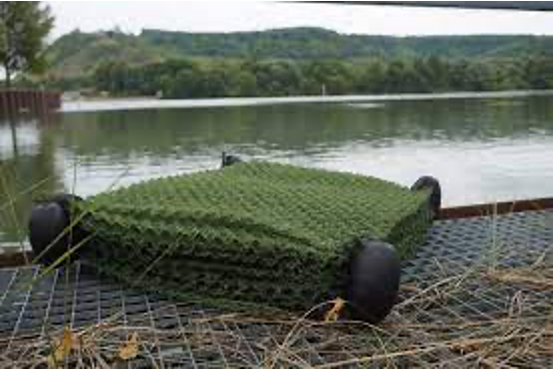
\includegraphics[width=0.5\textwidth]{Flottang}
\caption{Flottang (SEINORMIGR)}
\label{Flottang}
\end{figure}

\subsubsection{Protocole des flottangs}

Pour le suivi de cette année 2024, deux flottangs ont été mis en place. Le premier en aval de la passe à anguille en rive droite mais cette année un second a lui aussi été mis en place en aval de la passe à anguilles rive gauche. Les années précédentes un flottang était mis en place à l’amont de l’écluse rive droite pour mettre en évidence le passage des anguilles par l’écluse, mais les résultats ne donnant aucune réelle information, cette année ce flottang n’a pas été remis en place. La mise en place des flottangs permet de détecter des éventuelles accumulations d’anguilles au pied des passes du fait d’un dysfonctionnement de la rampe qui peut être un mauvais attrait, un problème d’alimentation en eau sur la rampe ou une vitesse de courant trop forte. La relève se fait à l’aide d’une corde attachée au flottang. La remontée se fait le plus rapidement possible afin d’éviter que des individus ne s’échappent. Une fois le flottang remonté, il est directement retourné dans un bac rectangulaire de dimension 60 cm x 40 cm. Pour permettre aux individus présents de tomber dedans et d’être récupéré. 

Les anguilles sont ensuite elles aussi anesthésiées, analysées (biométrie complète) puis relâchées en amont du barrage.

\subsubsection{Saisie et bancarisation des données }

Tout comme les pièges actifs, un carnet est dédié aux flottangs pour le terrain. Les paramètres renseignés sont les mêmes que les dispositifs actifs.
Ensuite, les données sont retranscrites dans un fichier Excel. Pour chaque année de suivi (depuis 2020), des tableaux croisés dynamiques produisent automatiquement des graphiques et tableaux actualisés. Ce dispositif  a été mis en place dans le cadre de cette étude.


\subsection{Paramètres environnementaux}

De nombreux auteurs ont montré l’importance des facteurs environnementaux dans la migration des anguilles et plus particulièrement des civelles en estuaire \citep{todd_timing_1981, white_environmental_1997, bardonnet_influence_2003, feunteun_review_2003}. De multiples paramètres environnementaux ont été choisis comme pouvant potentiellement contribuer à la migration en Seine, au barrage de Poses. Ces paramètres sont relevés :

Température (°C) de l’eau : Une sonde thermique automatique (modèle "Onset HOBO UA-001-64 PendantTemp") relève la température toutes les heures, en amont de la rampe à anguille en rive droite. Une sonde appartenant au GIPSA situé à Rouen est aussi active en sécurité si la première sonde rencontre un problème et ne fonctionne plus.

Température (°C) de l’air : Données tirées du site internet : météo.france.fr. La station de mesure est située à Muids (indisponible à Poses).

Coefficient de marée : Données tirées du site internet : maree.shom.fr. Le Shom est un établissement public à caractère administratif, placé sous la tutelle du ministère des Armées (shom.fr). Le port de référence est situé au Havre. 

Débit moyen journalier (QmJ - m3/s) : Données tirées du site internet : hydro.eaufrance.fr. La station de mesure est située à Vernon (indisponible à Poses). 

\subsection{Traitement de données }

\subsubsection{Analyse globale }

\textbf{Indice pathologique (lpG) et indice parasitaire (IpP) :} 


Les codes pathologiques sont utilisés pour calculer l’IpG et l’IpP, indices évaluant la qualité de l’habitat et l’état de santé des peuplements piscicoles \citep{elie_sante_2014} (Figure \ref{Grille}). L’indice pathologique (s’applique uniquement aux lésions) considère trois paramètres : 

\begin{figure}[htpb]
\centering
\includegraphics[width=\textwidth]{Grille}
\caption{Grille de codification des anomalies anatomo-morphologiques externes et des ectoparasites des poissons visibles à l'oeil nu. \citep{elie_sante_2014}}
\label{Grille}
\end{figure}

1.	(i)  Prévalence des poissons présentant des lésions externes : P (\%) = (nb poissons avec lésions) / (nb poissons examinés) 

2.	(ii)  Intensité lésionnelle : Q = La notation va de 0 (absence de lésions) à 4 (plus de 10 lésions ou plus de 20\% de recouvrement corporel). 

3.	(iii) Signification écopathologique des lésions : S = 1 pour les lésions mineures et 2 pour les lésions majeures (déformations, tumeurs, érosions, nécroses, hémorragies, ulcères). 

Pour une même pathologie (x), l’indice s’exprime comme suit : IIII(xx) = P(x) × Q(x) × S(x). Pour une population donnée, les Ip relatifs à chaque lésion sont additionnés : $ \mathrm{I}_{pG}^{} = \sum_{}^{}\mathrm{I}_{p}^{} $


L’indice parasitaire (s’applique uniquement aux parasites) est calculé de la même manière mais ne prend pas en compte la signification écopathologique (S). Le résultat de ces indices est interprété selon la grille (Figure \ref{Interprétation}).

\begin{figure}[htpb]
\centering
\includegraphics[width=\textwidth]{Interprétation}
\caption{Grille d'interprétation de l'indice pathologique (IpG) et parasitaire (IpP) \citep{elie_sante_2014}}
\label{Interprétation}
\end{figure}

\subsubsection{Analyses statistiques}
	
Pour analyser nos résultats, des traitements ont été fait à partir du logiciel R studio.
Tout d’abord, les tests de comparaison utilisés ont été le test de Student pour 2 échantillons et L’ANOVA pour 3 échantillons ou plus. Pour chaque test, sont toujours vérifiés la normalité ainsi que l’homogénéité. Si les résultats sont significatifs, un test de comparaison multiple va nous montrer le ou les échantillons différents.
Un autre test utilisé est l’analyse en composante principale (ACP). Cela est utilisé pour identifier les différents paramètres exerçant une influence sur la migration. En complémentarité, un test de corrélation est réalisé sur chaque paramètre par rapport aux effectifs d’anguilles. Pour finir, un test de significativité du R2 est appliqué.


\section{Résultats}

\textit{Note : Les résultats qui vont vous être présentés dans cette partie concernent les données du 2 avril au 23 septembre 2024.}

\subsection{Bilan migratoire 2024 }

Pour cette année 2024, le suivi a commencé le 2 avril, jour de la mise en route des pièges à anguilles. Les pièges de la rive droite aussi bien que la rive gauche ont fonctionné sans interruption pendant la période de suivi. Les premiers individus ont été observés le 8 avril en rive droite mais aussi en rive gauche. Les premiers individus de l’année avec une taille d’environ 80 mm ont été observés le 8 juillet. Pour cette année 2024, du 2 avril au 23 septembre un total de 846 545 anguilles a été comptabilisé soit un total de 85 017 (90\%) en rive droite et de 761 528 (10\%) en rive gauche. La (Figure \ref{graph_oral}) représente les effectifs journaliers ainsi que les effectifs cumulés, deux pics sont visibles avec un premier début août et le principal mi-août que cela soit pour la rive droite ou la rive gauche. Cette année encore les anguilles ont majoritairement emprunté la rive droite par rapport à la rive gauche.


\begin{figure}[htpb]
\centering
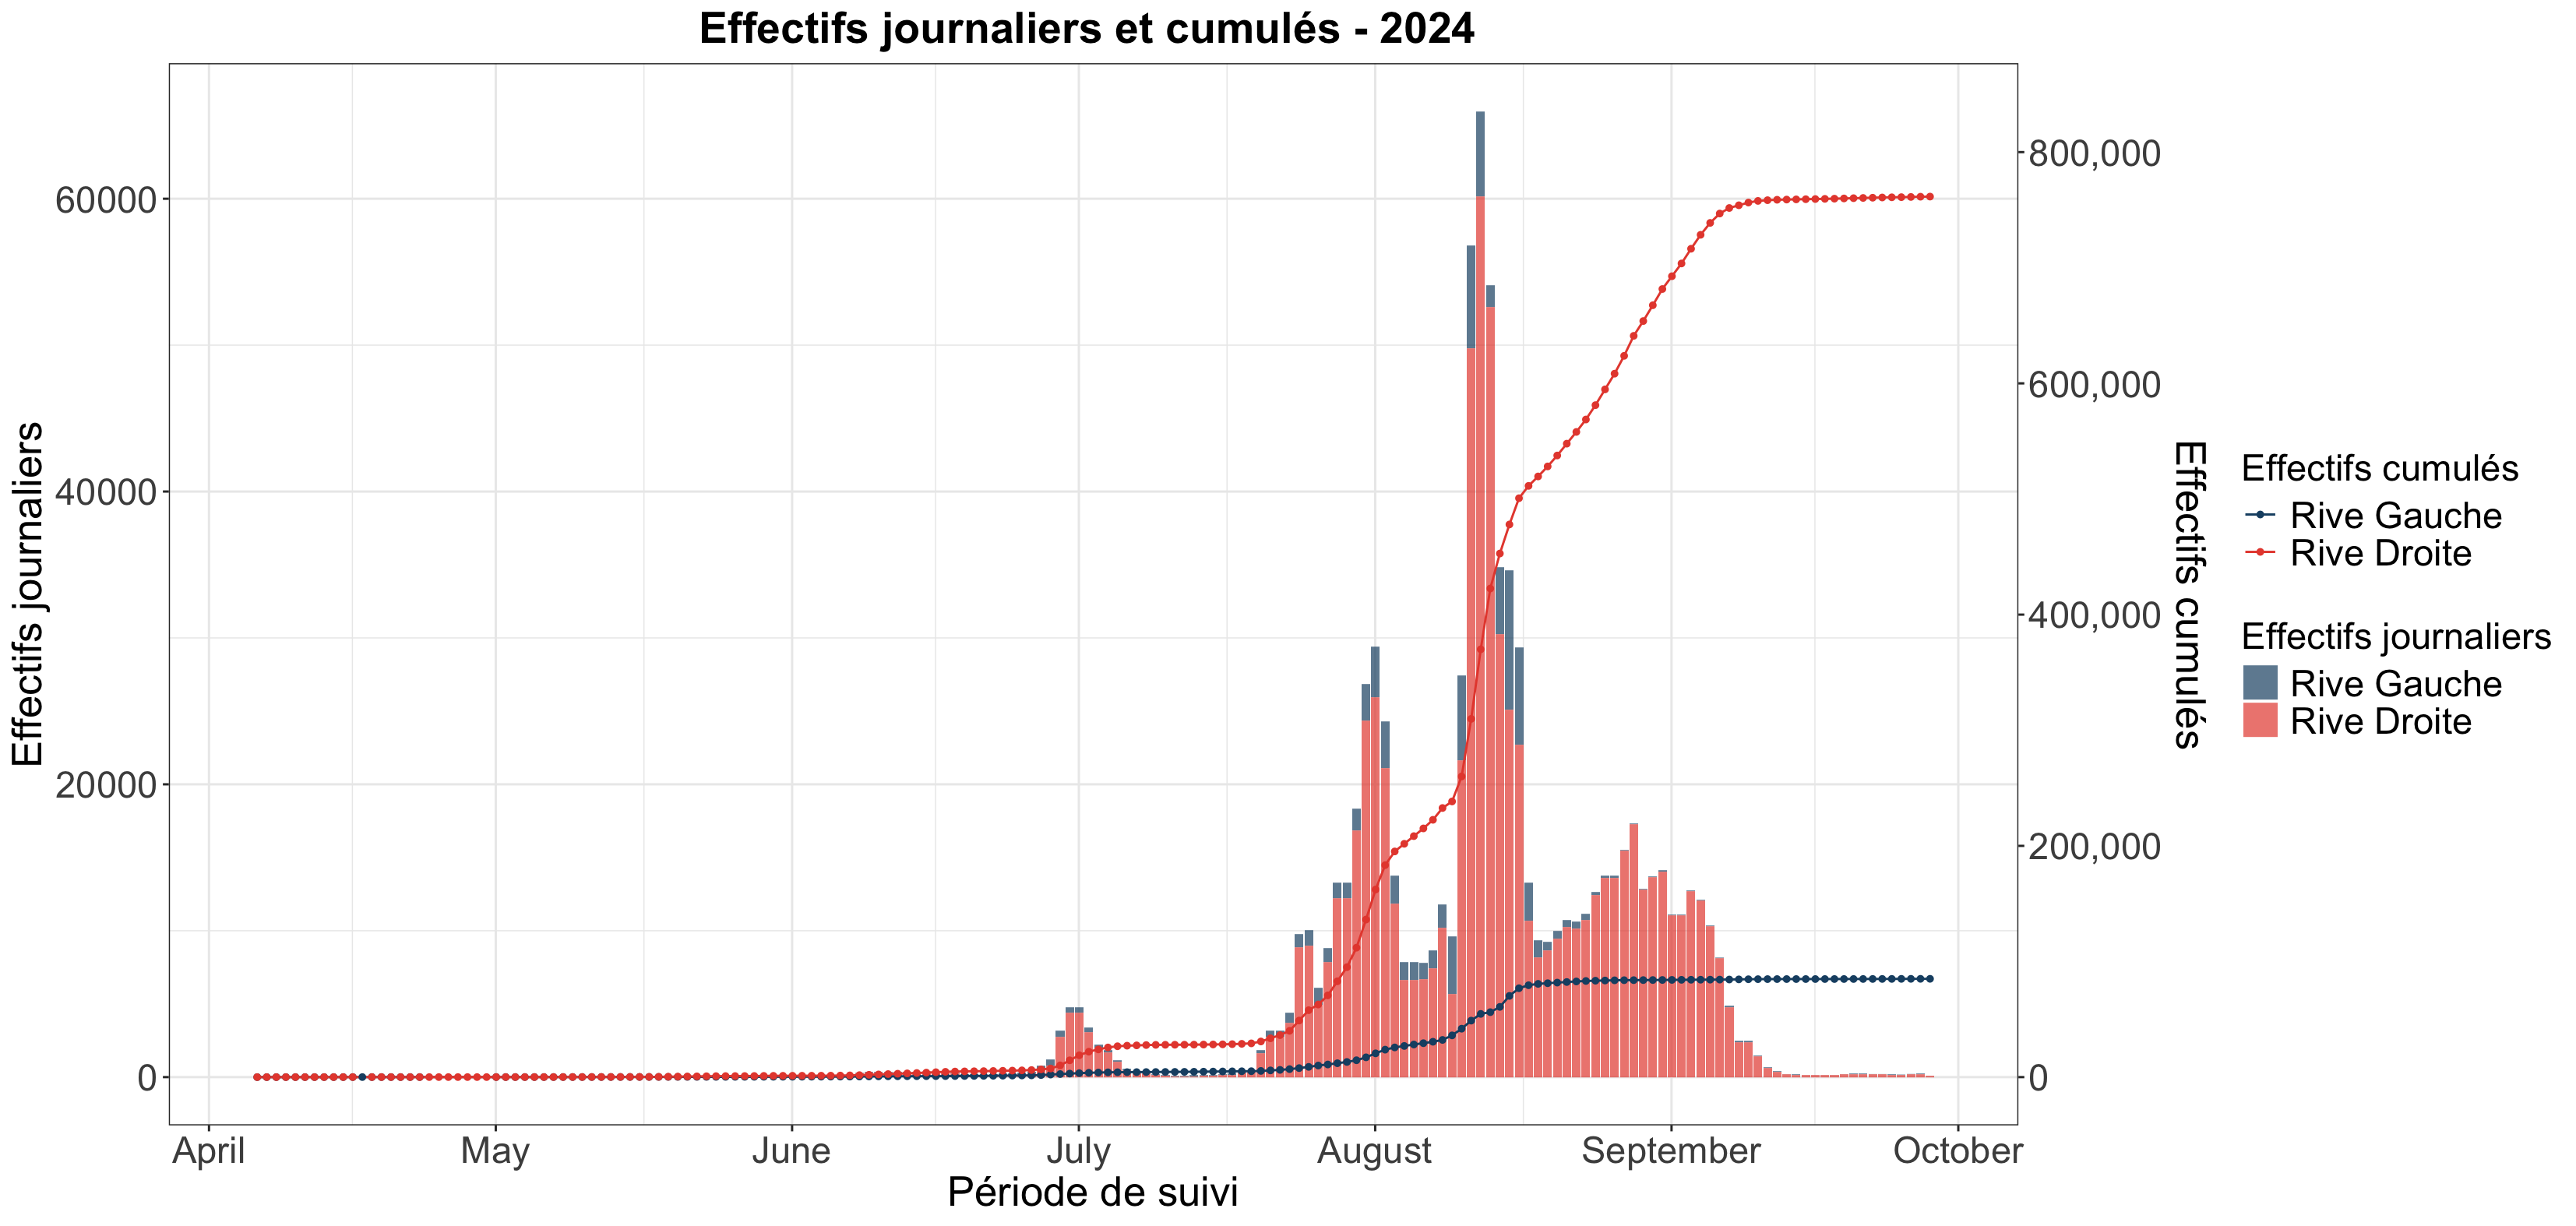
\includegraphics[width=\textwidth]{graph_oral.png}
\caption{Effectifs journaliers et cumulés des deux rives en 2024}
\label{graph_oral}
\end{figure}

\subsection{Comparaisons interannuelles des migrations}

Le suivi du recrutement des anguilles européennes en Seine est réalisé sur le barrage de Poses depuis 2014 en rive gauche et depuis 2018 en rive droite.  Cette année, les résultats obtenus sur la migration sont les plus importants depuis la mise en place du suivi (Figure \ref{graph_annee_oral}). Les (Figure \ref{g_RG}) et (Figure \ref{g_RD}) présentent les dynamiques de migration par rive. Les graphiques mettent en évidence des effectifs cumulés interannuels. 


\begin{figure}[htpb]
\centering
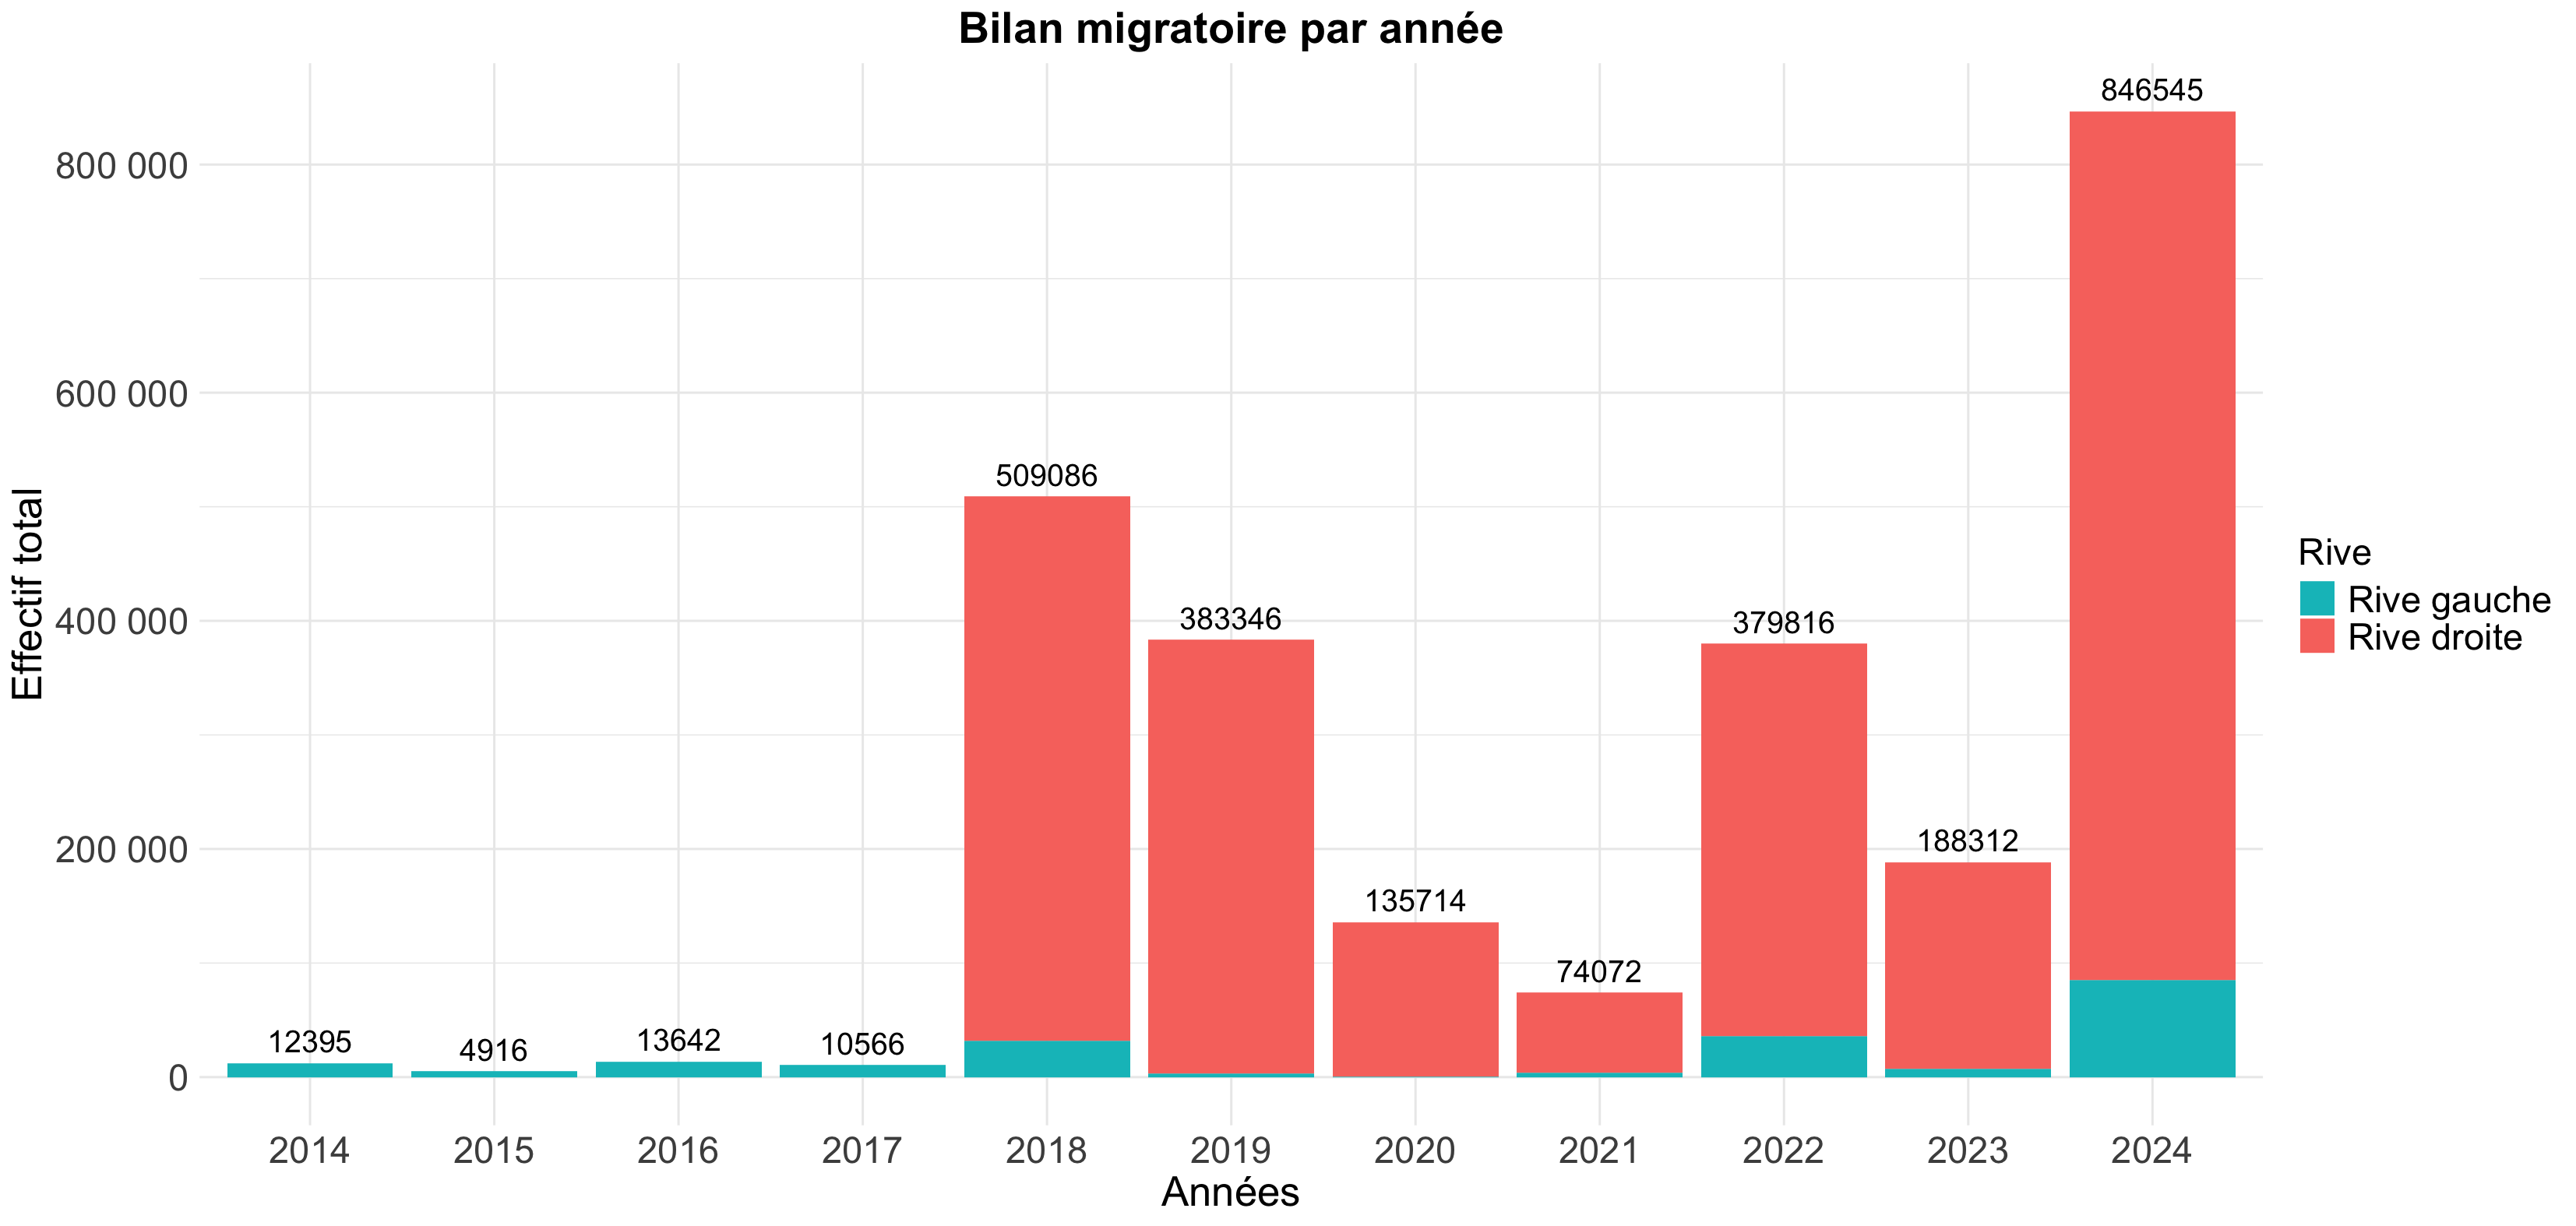
\includegraphics[width=\textwidth]{graph_annee_oral.png}
\caption{Évolution interannuelle des effectifs des anguilles capturées dans les pièges}
\label{graph_annee_oral}
\end{figure}

\begin{figure}[htpb]
\centering
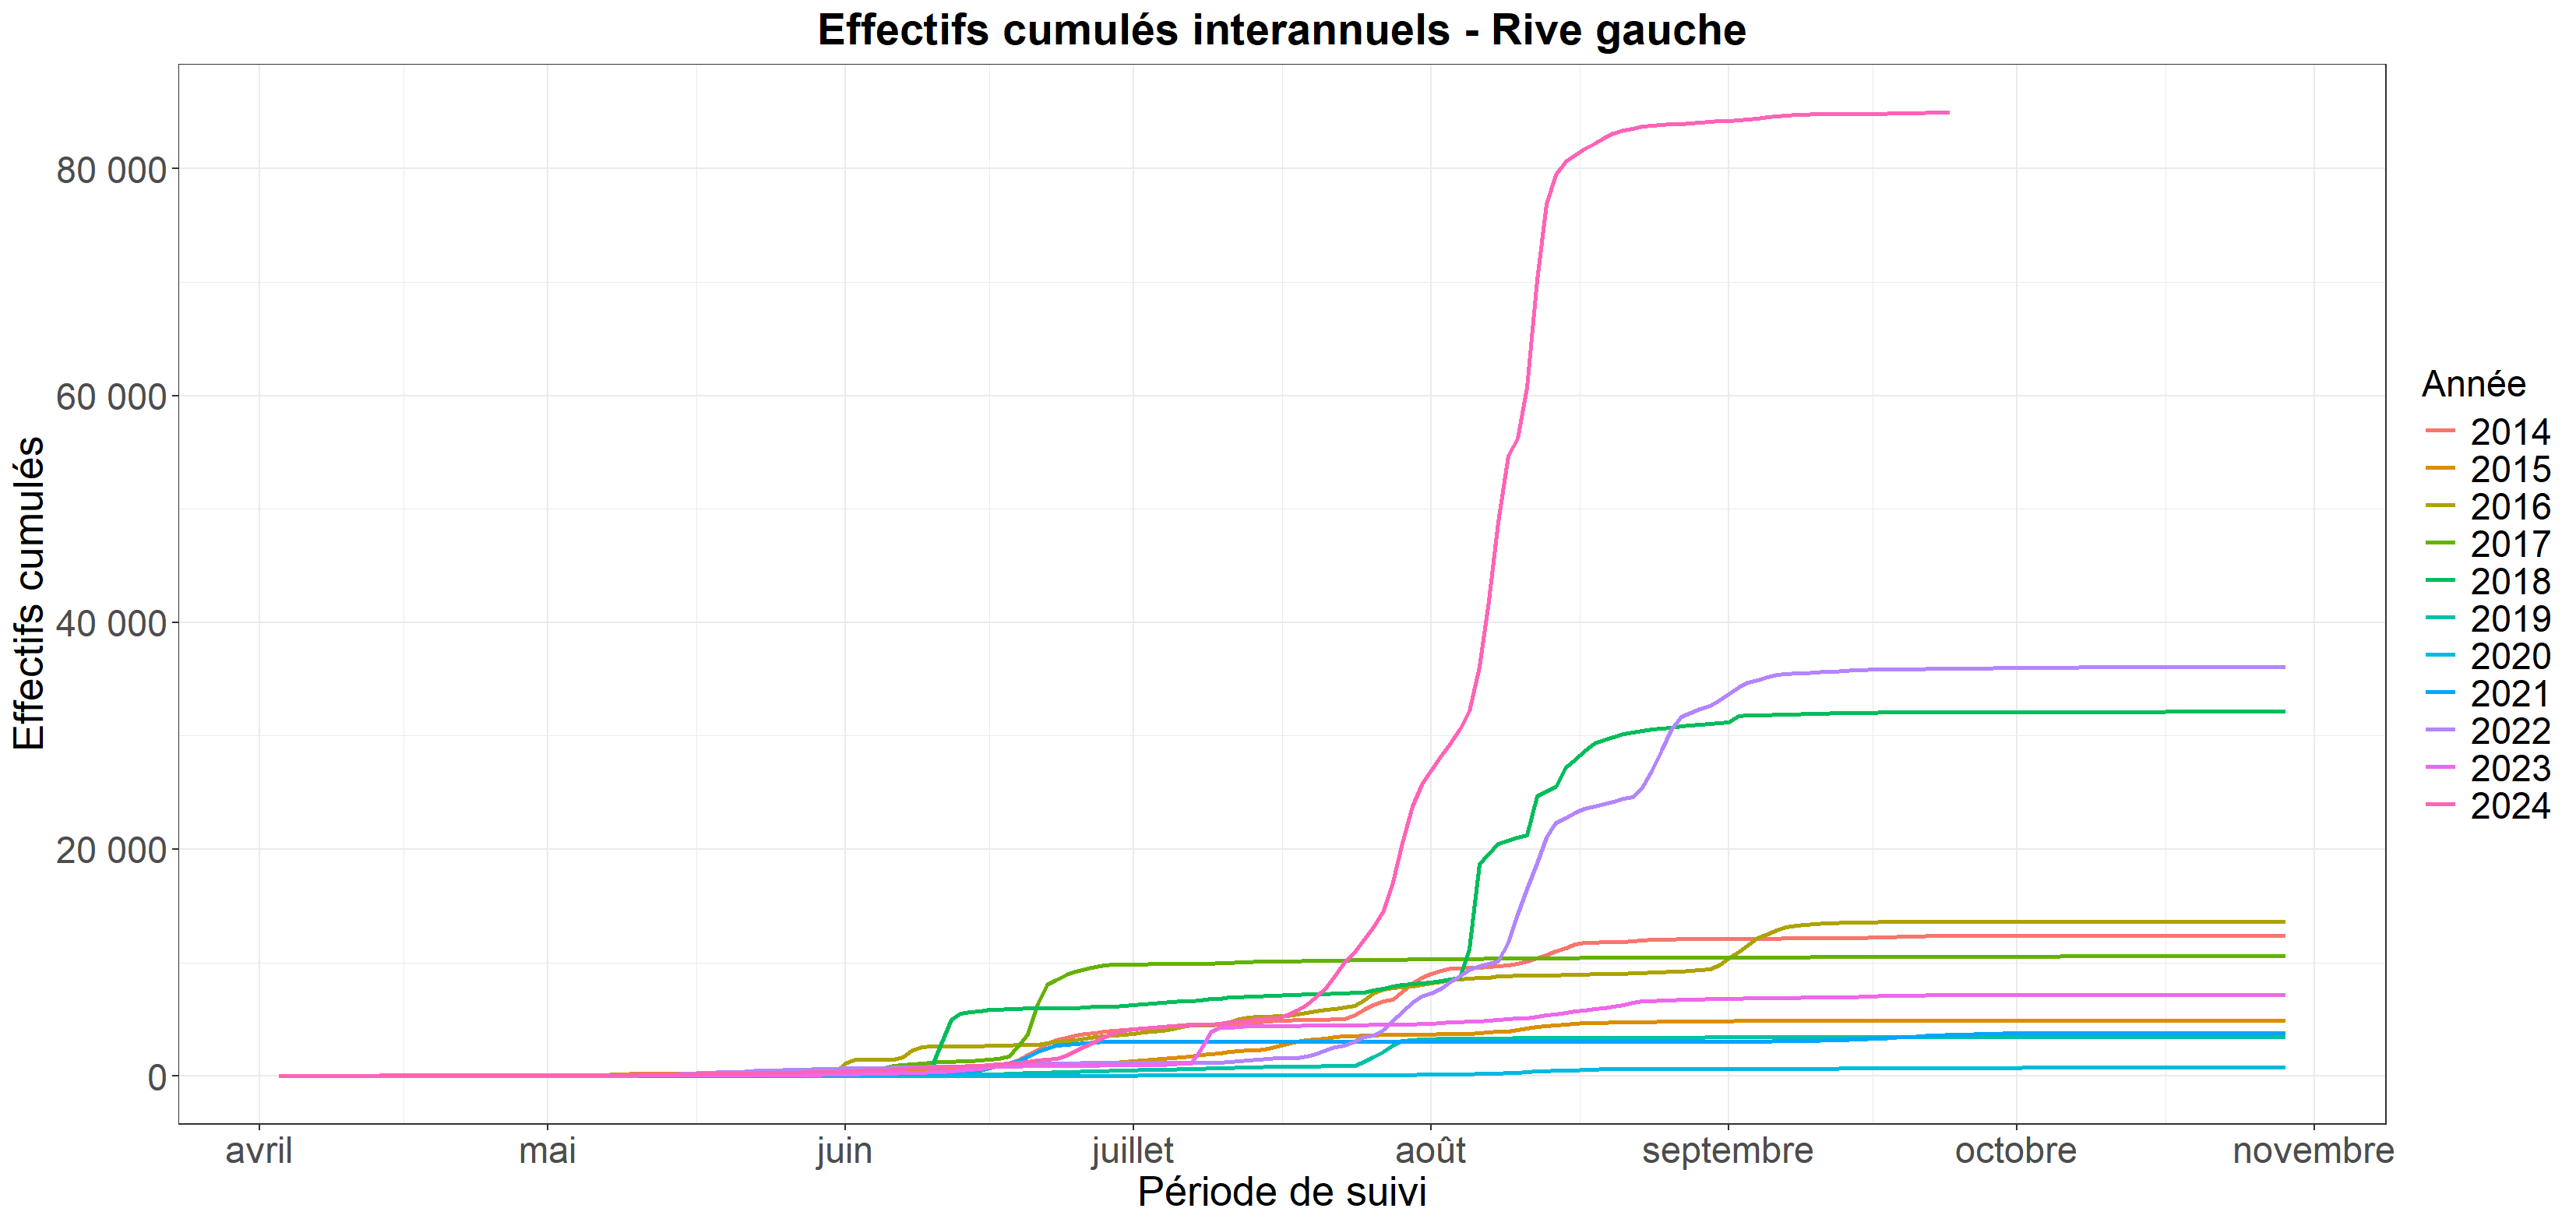
\includegraphics[width=\textwidth]{g_RG.png}
\caption{Effectifs cumulés rive gauche}
\label{g_RG}
\end{figure}

Tout d’abord, sur la (Figure \ref{g_RG}) concernant la rive gauche, nous pouvons observer que les dynamiques de migrations sont relativement similaires avec des captures faibles en début de saison. Les captures augmentent ensuite progressivement jusqu’à des pics de migrations.   Ces pics de migrations ont souvent lieu l’été en juillet-août cependant il y a une forte variabilité entre les années en termes d’effectifs.

A noté que pour cette année en rive gauche, 761 528 anguilles ont été piégées, soit plus du double des effectifs de l’année 2020 qui était jusqu’à présent la meilleure année.


La (Figure \ref{g_RD}) concerne la rive droite, nous pouvons observer que là aussi les dynamiques de migrations sont similaires en début de saison avec des captures relativement basses. Tout comme en rive gauche les captures augmentent ensuite progressivement jusqu’à des pics de migrations. Cependant, en rive droite contrairement à la rive gauche les pics de migrations commencent mi-juillet pour chaque année jusqu’à mi-août début septembre pour certaines années. Cette année en rive droite 85 017 anguilles ont été piégées, en comparaison l’année 2018 a comptabilisé 476 958 individus sur toute la période de suivi.

\begin{figure}[htpb]
\centering
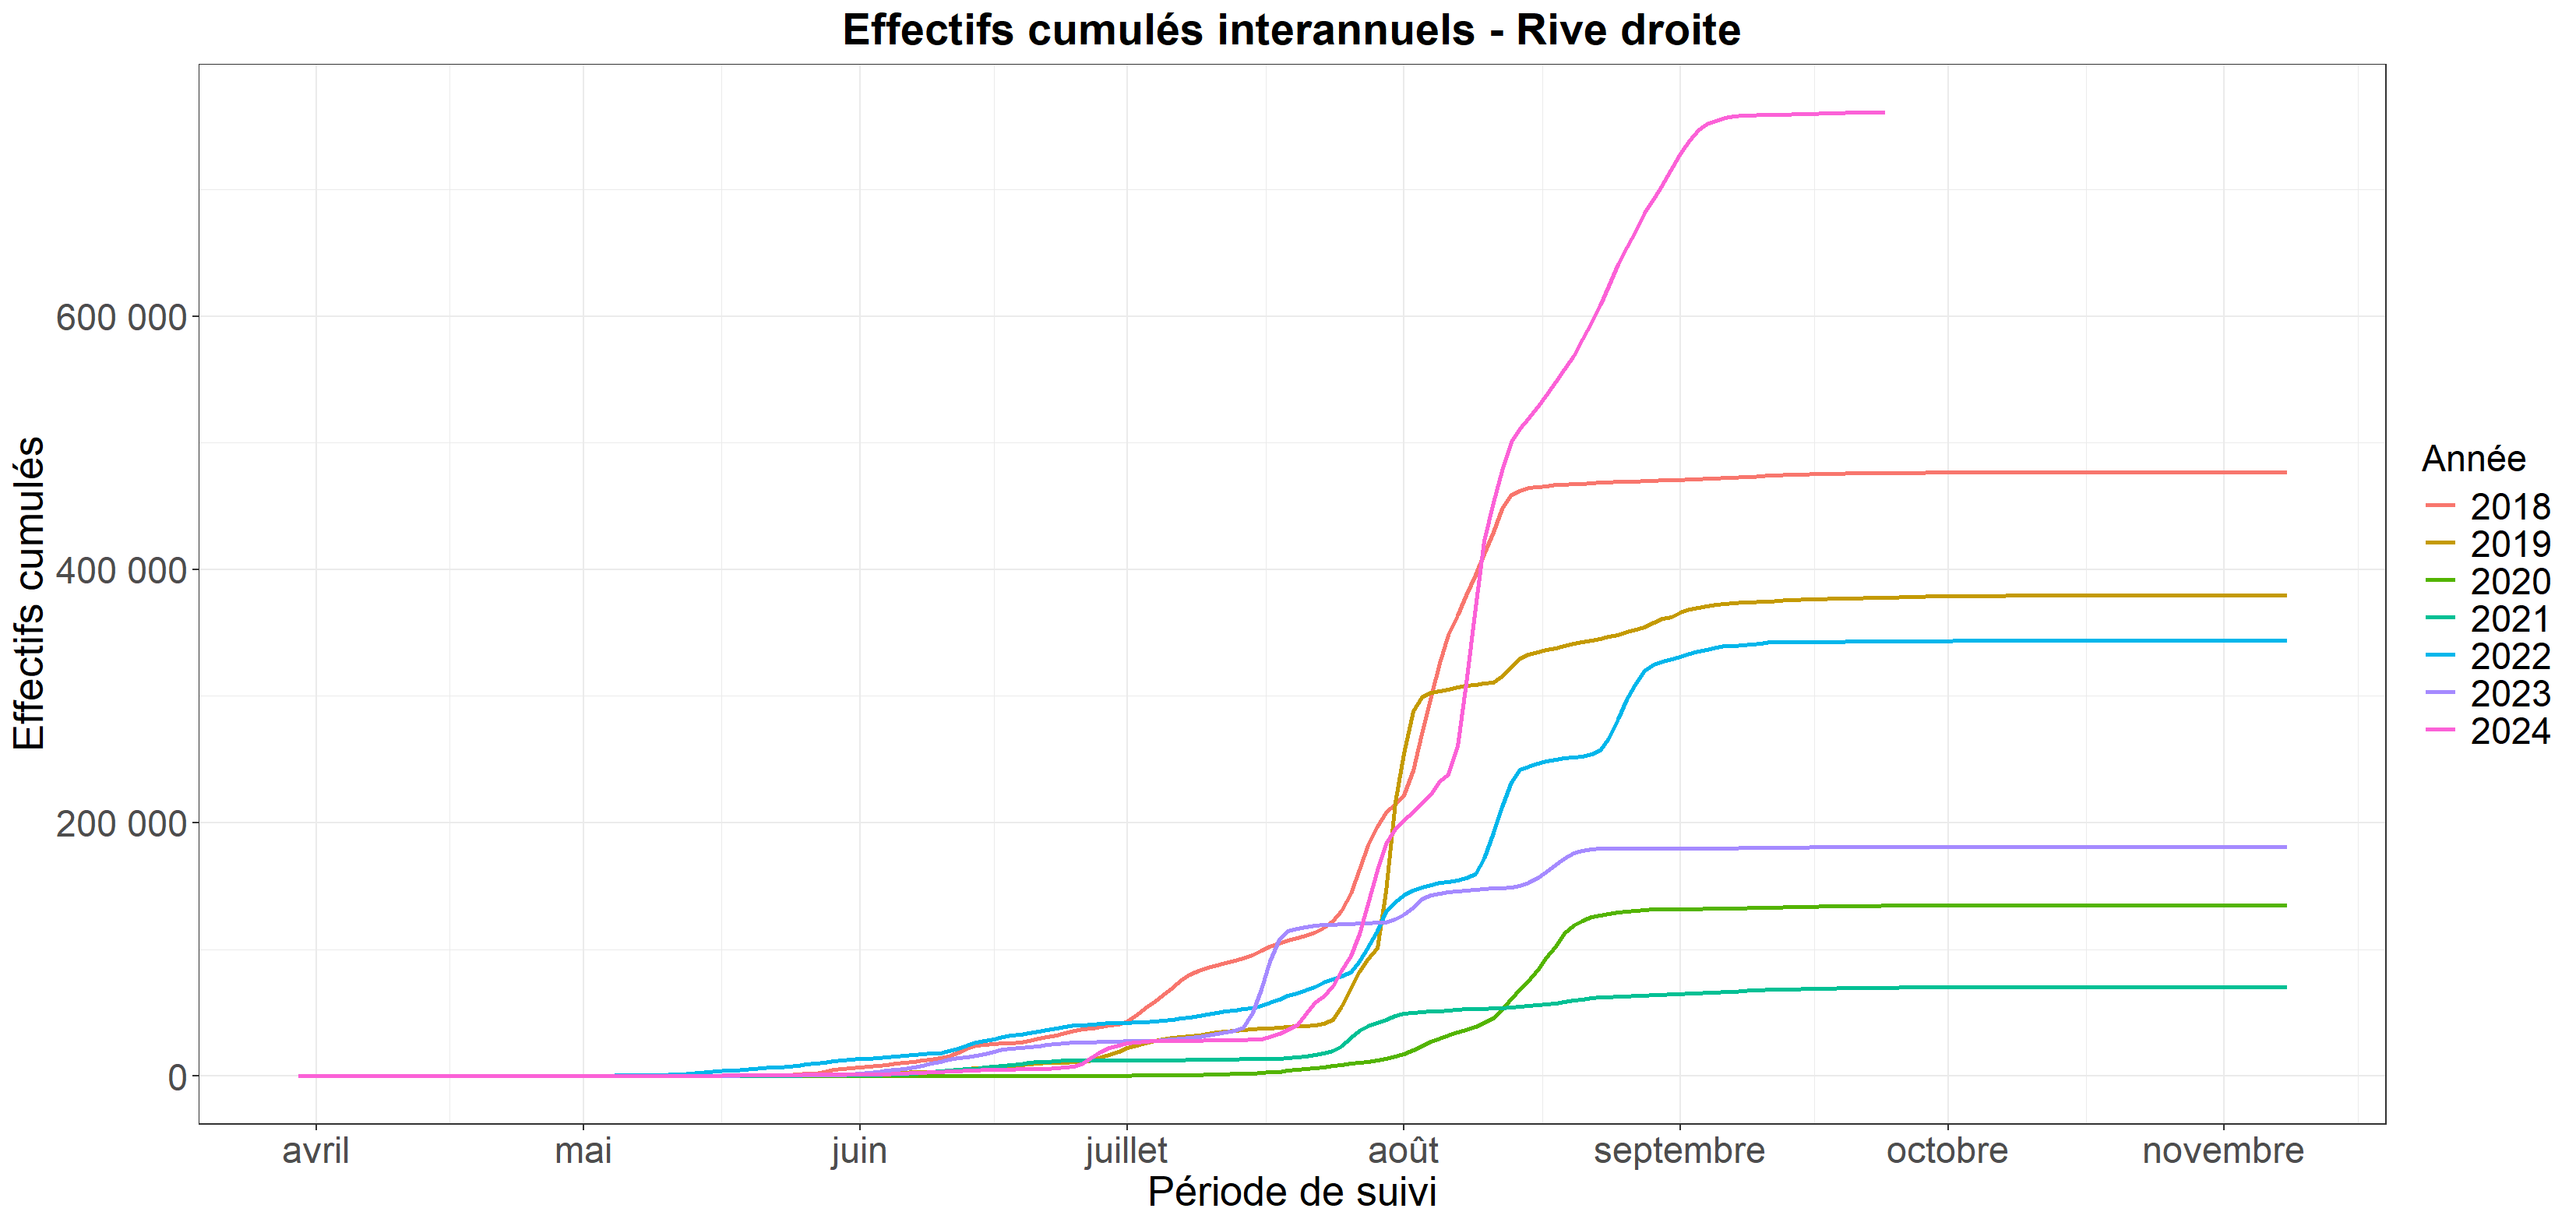
\includegraphics[width=\textwidth]{g_RD.png}
\caption{Effectifs cumulés rive gauche}
\label{g_RD}
\end{figure}


\subsection{Morphotypes des individus en 2024}

\subsubsection{Tailles selon la rive}

\textit{Note : les données de taille ne concernent que les individus biométrés. }

La (Figure \ref{taille_oral}) présente la taille des individus biométrés en mm sur les deux rives. Nous pouvons voir que pour les deux rives la majorité des individus ont une taille d’environ 80 mm ce qui correspond aux anguillettes de l’année. Peu d’individus en rive gauche dépassent les 250 mm alors qu’en rive droite certains individus dépassent les 300 mm voir les 400 mm dans des cas très rare. En rive gauche la taille moyenne est de 105 mm avec une médiane de 87 mm alors qu’en rive droite la taille moyenne des individus est de 111 mm avec une médiane a 90mm. Les individus empruntant la rive gauche sont significativement plus petits que ceux de la rive droite (wilcox-test, p < 0,05). Ce résultat est obtenu pour la première fois depuis le début des suivis, les années précédentes, les anguilles passant en rive gauche étaient plus grosses que les individus passant en rive droite (Figure \ref{taille_annee_oral}). Durant les relevés des pièges beaucoup d’individus de l’année ont été retrouvés en rive gauche ce qui n’étaient pas le cas les années précédentes. En rive droite de nombreuses anguilles ayant déjà plusieurs années donc en reprise de migration ont été retrouvées en quantité plus élevé surtout durant le mois de juillet contrairement aux années précédentes. 

\begin{figure}[htpb]
\centering
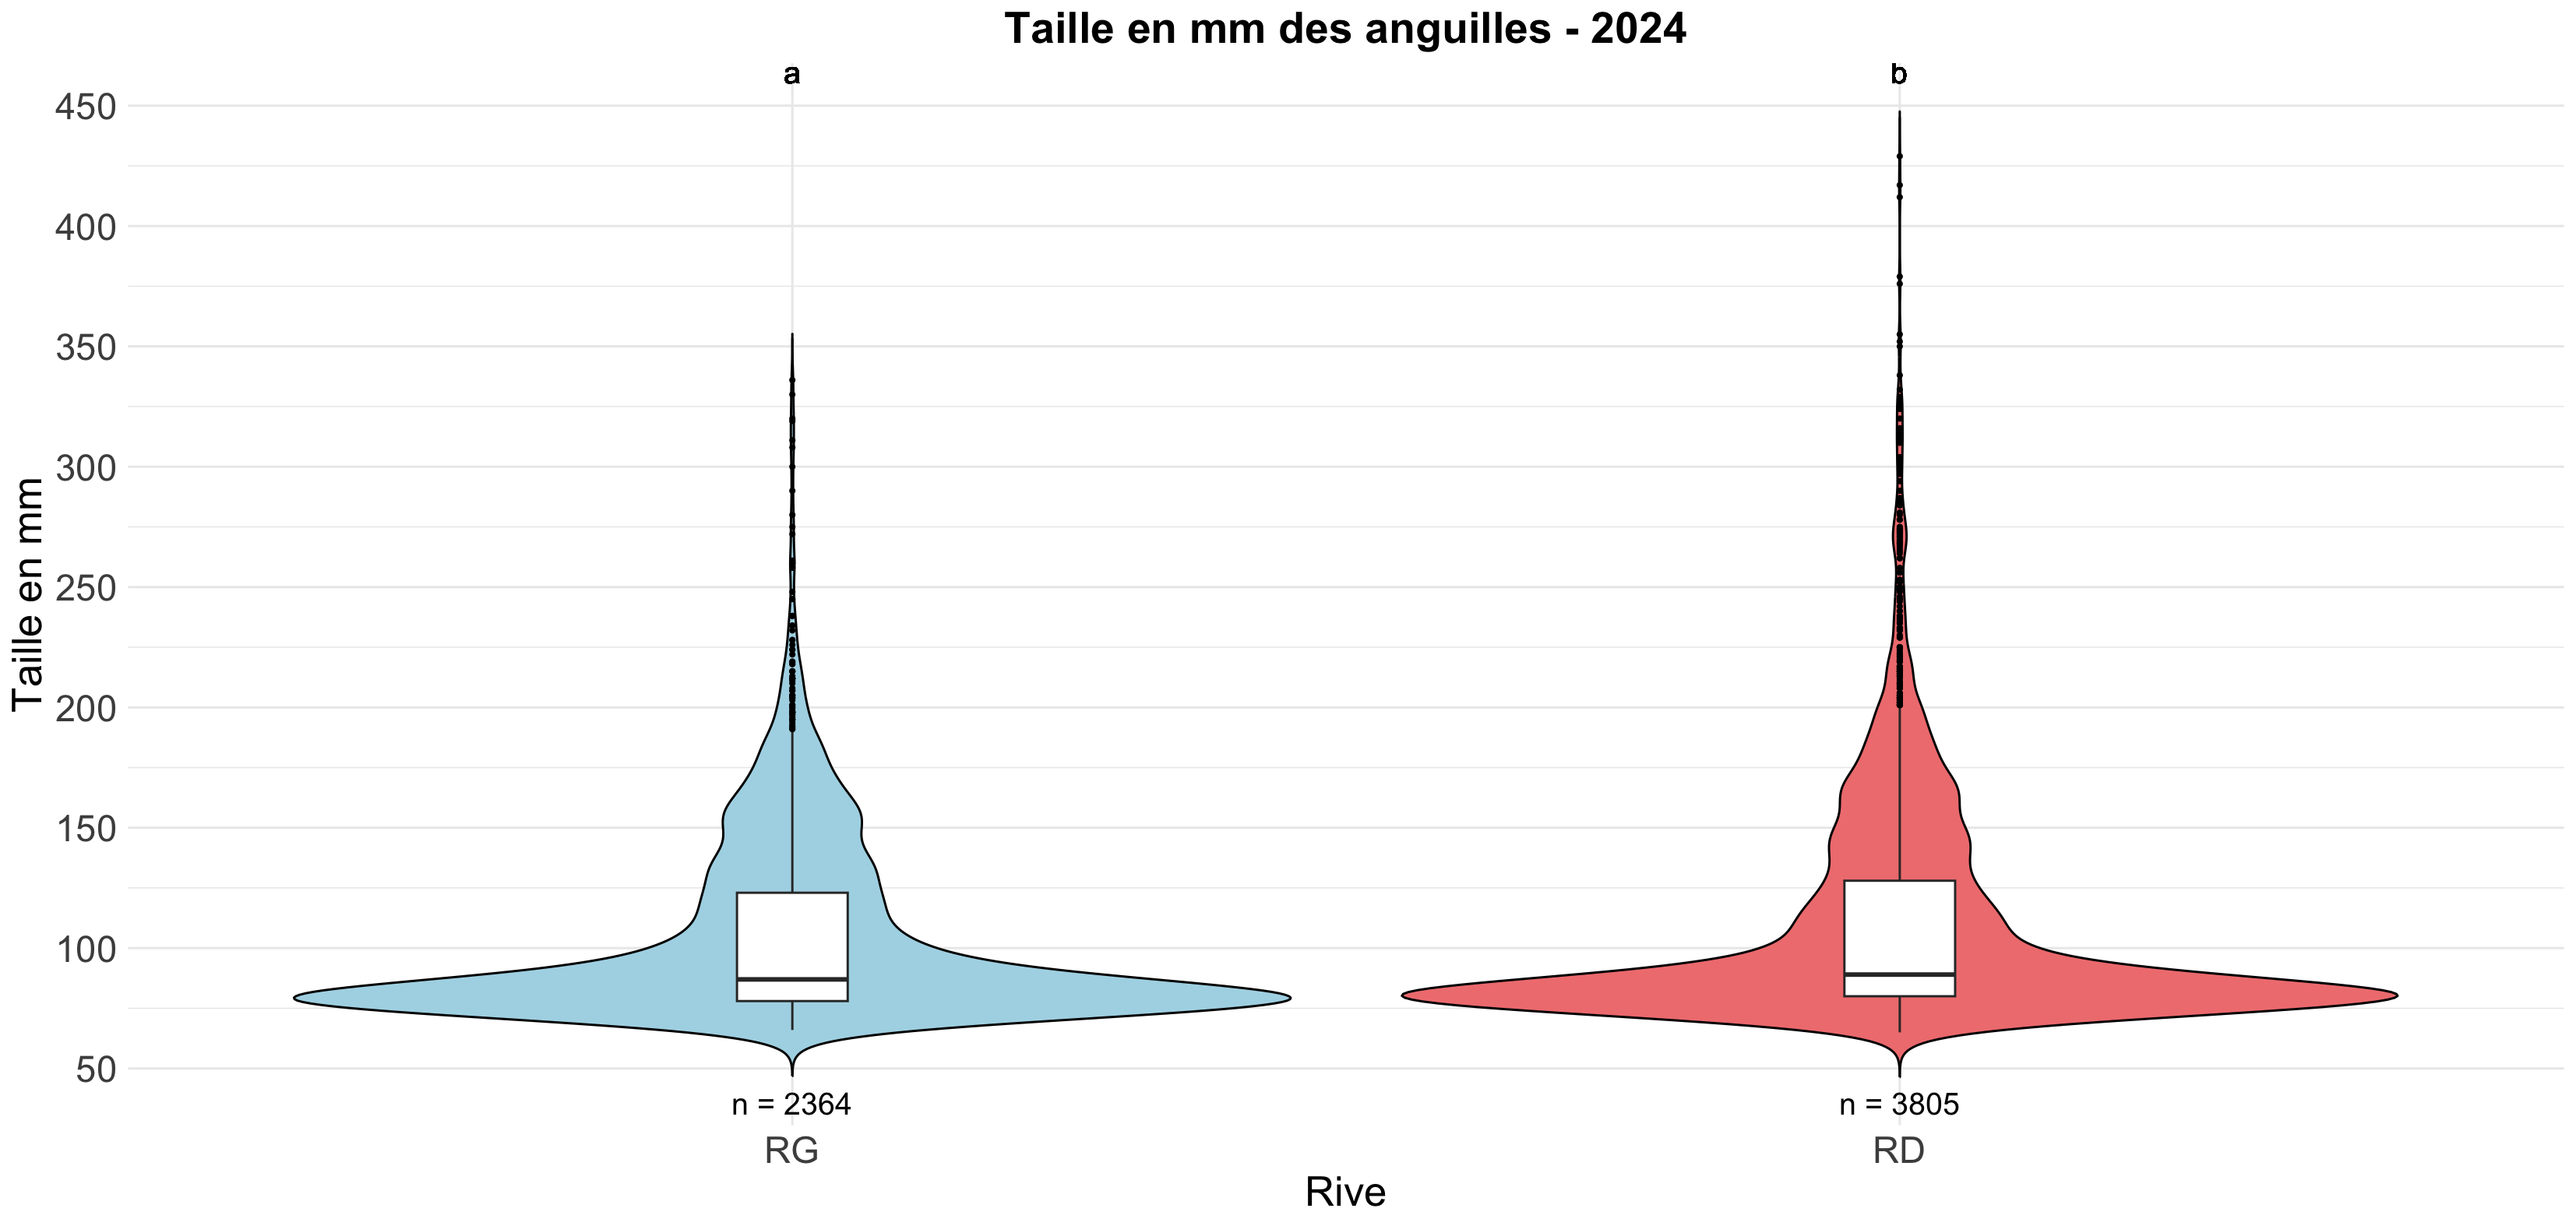
\includegraphics[width=\textwidth]{taille_oral.png}
\caption{Taille en mm des anguilles en rive droite et rive gauche - 2024}
\label{taille_oral}
\end{figure}

\begin{figure}[htpb]
\centering
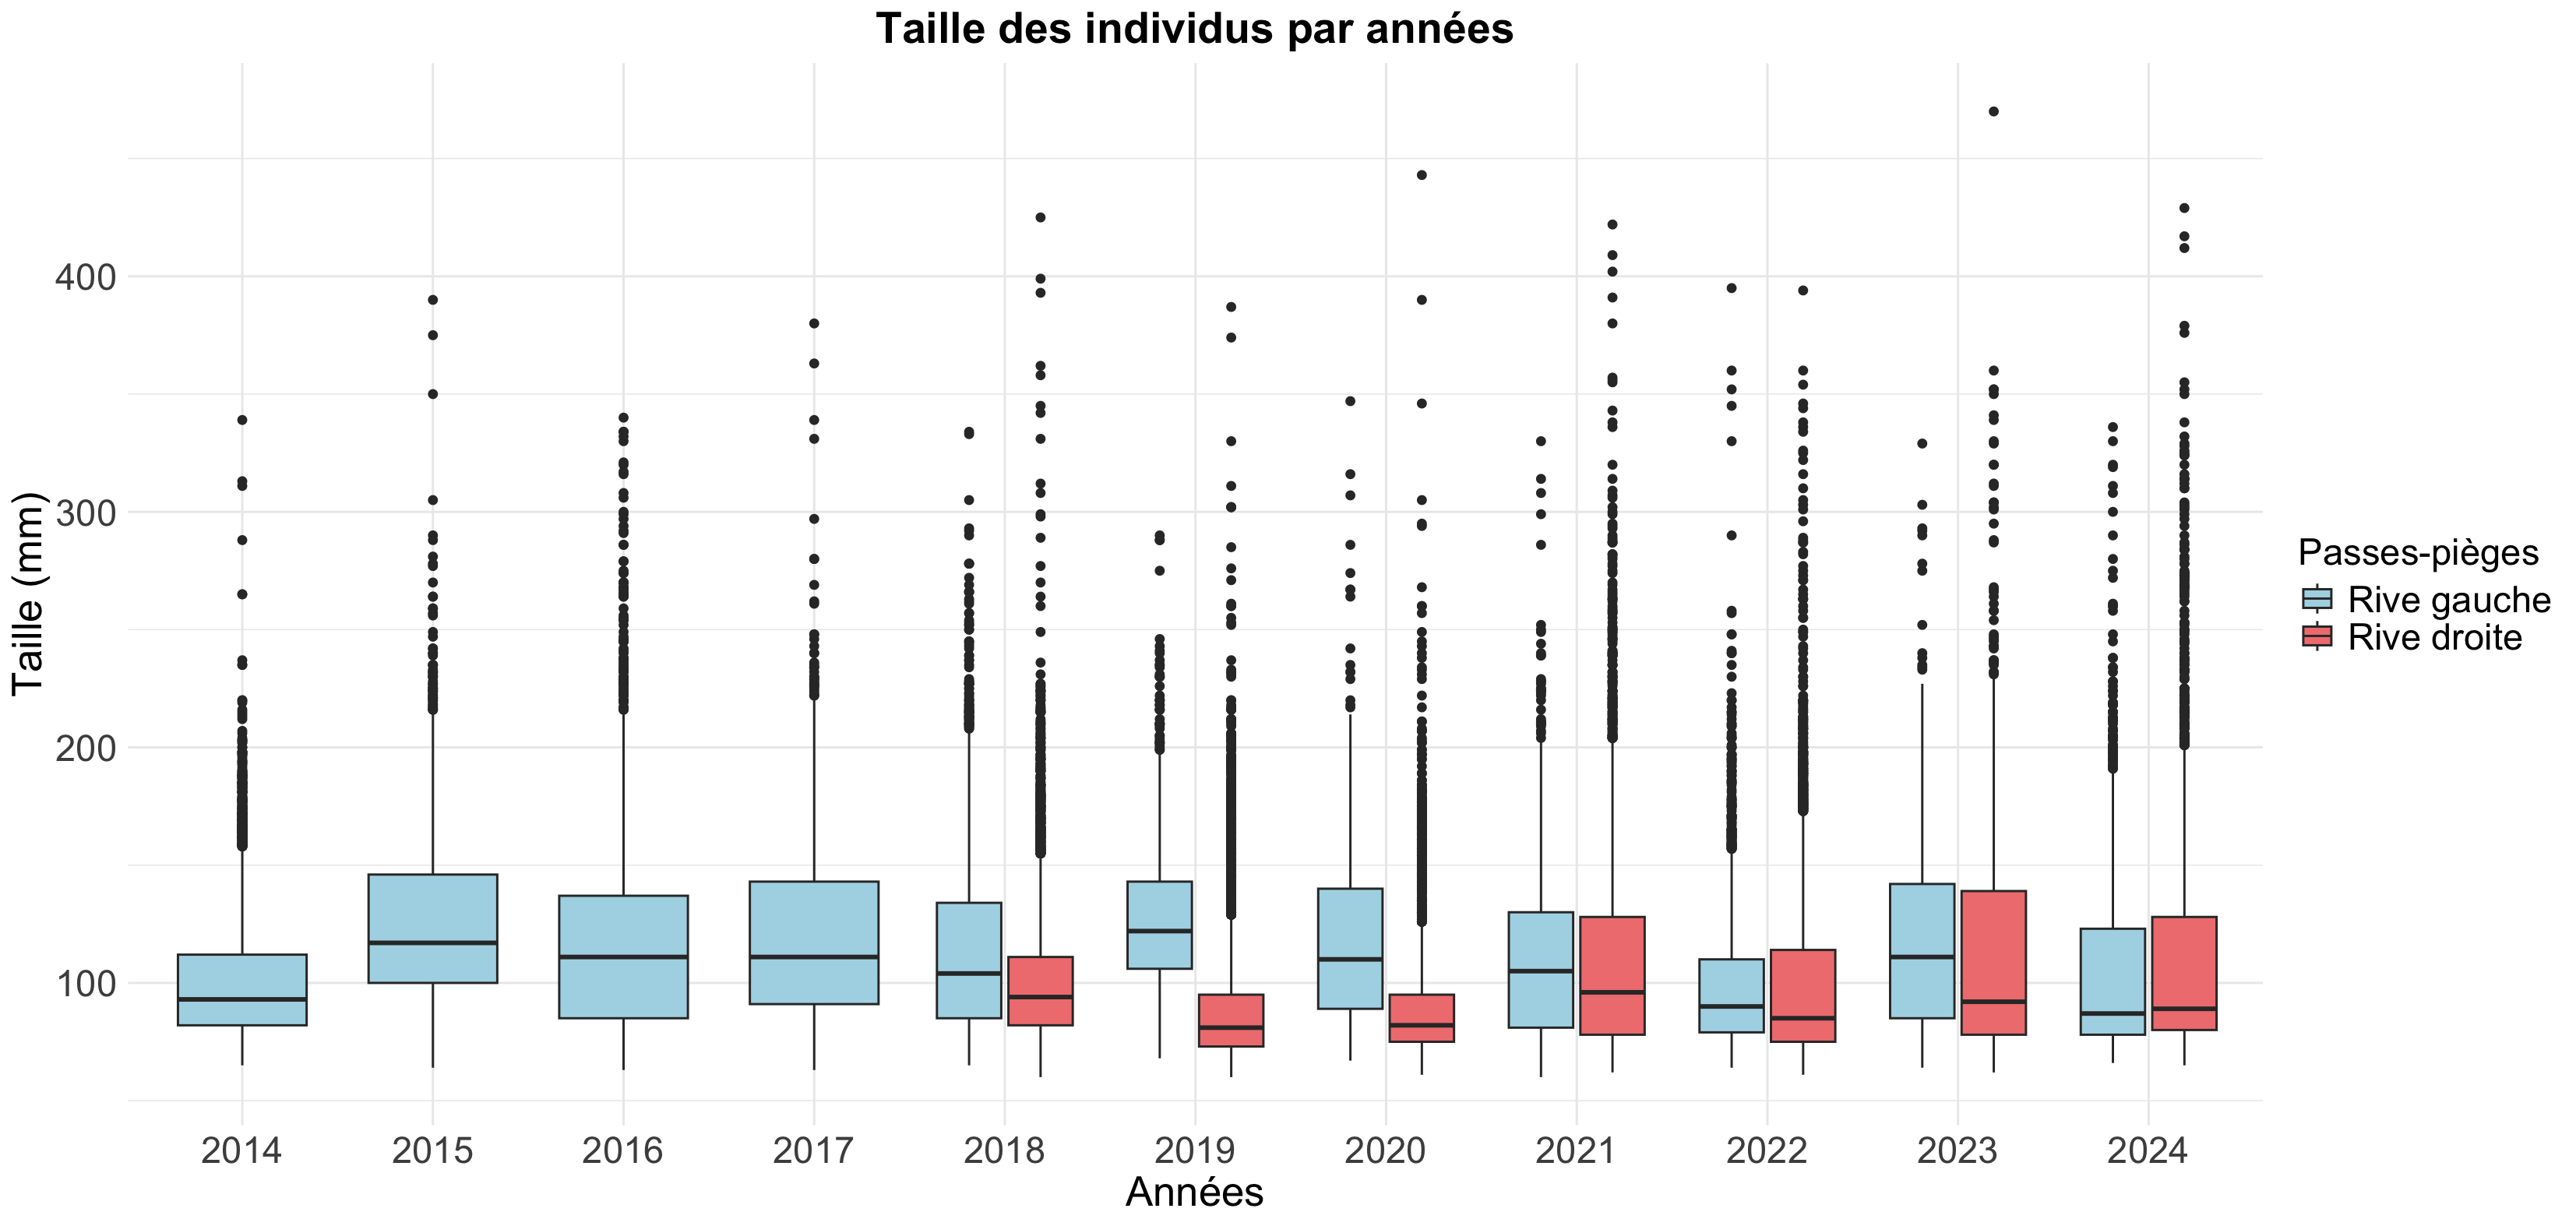
\includegraphics[width=\textwidth]{taille_annee_oral.png}
\caption{Taille en mm des anguilles en montaison par année en fonction de la rive}
\label{taille_annee_oral}
\end{figure}


La (Figure \ref{classe_taille_oral}) présente des classes de tailles des anguilles pour les deux rives. Ce résultat vient compléter la (Figure \ref{taille_oral}) car nous pouvons voir que les individus <= 85 mm (les individus de l’année), représentent 42\% des effectifs en rive gauche contre 30\% en rive droite. Les individus mesurant entre 85 et 115 mm représentent en rive gauche 20\% des effectifs et 24\% en rive droite. En rive droite, plus de 6\% des effectifs sont des individus de plus de 200 mm. En combinant les deux rives, les individus de l’année représentent 38\% des captures, ce résultat est similaire aux années précédentes. 


\begin{figure}[htpb]
\centering
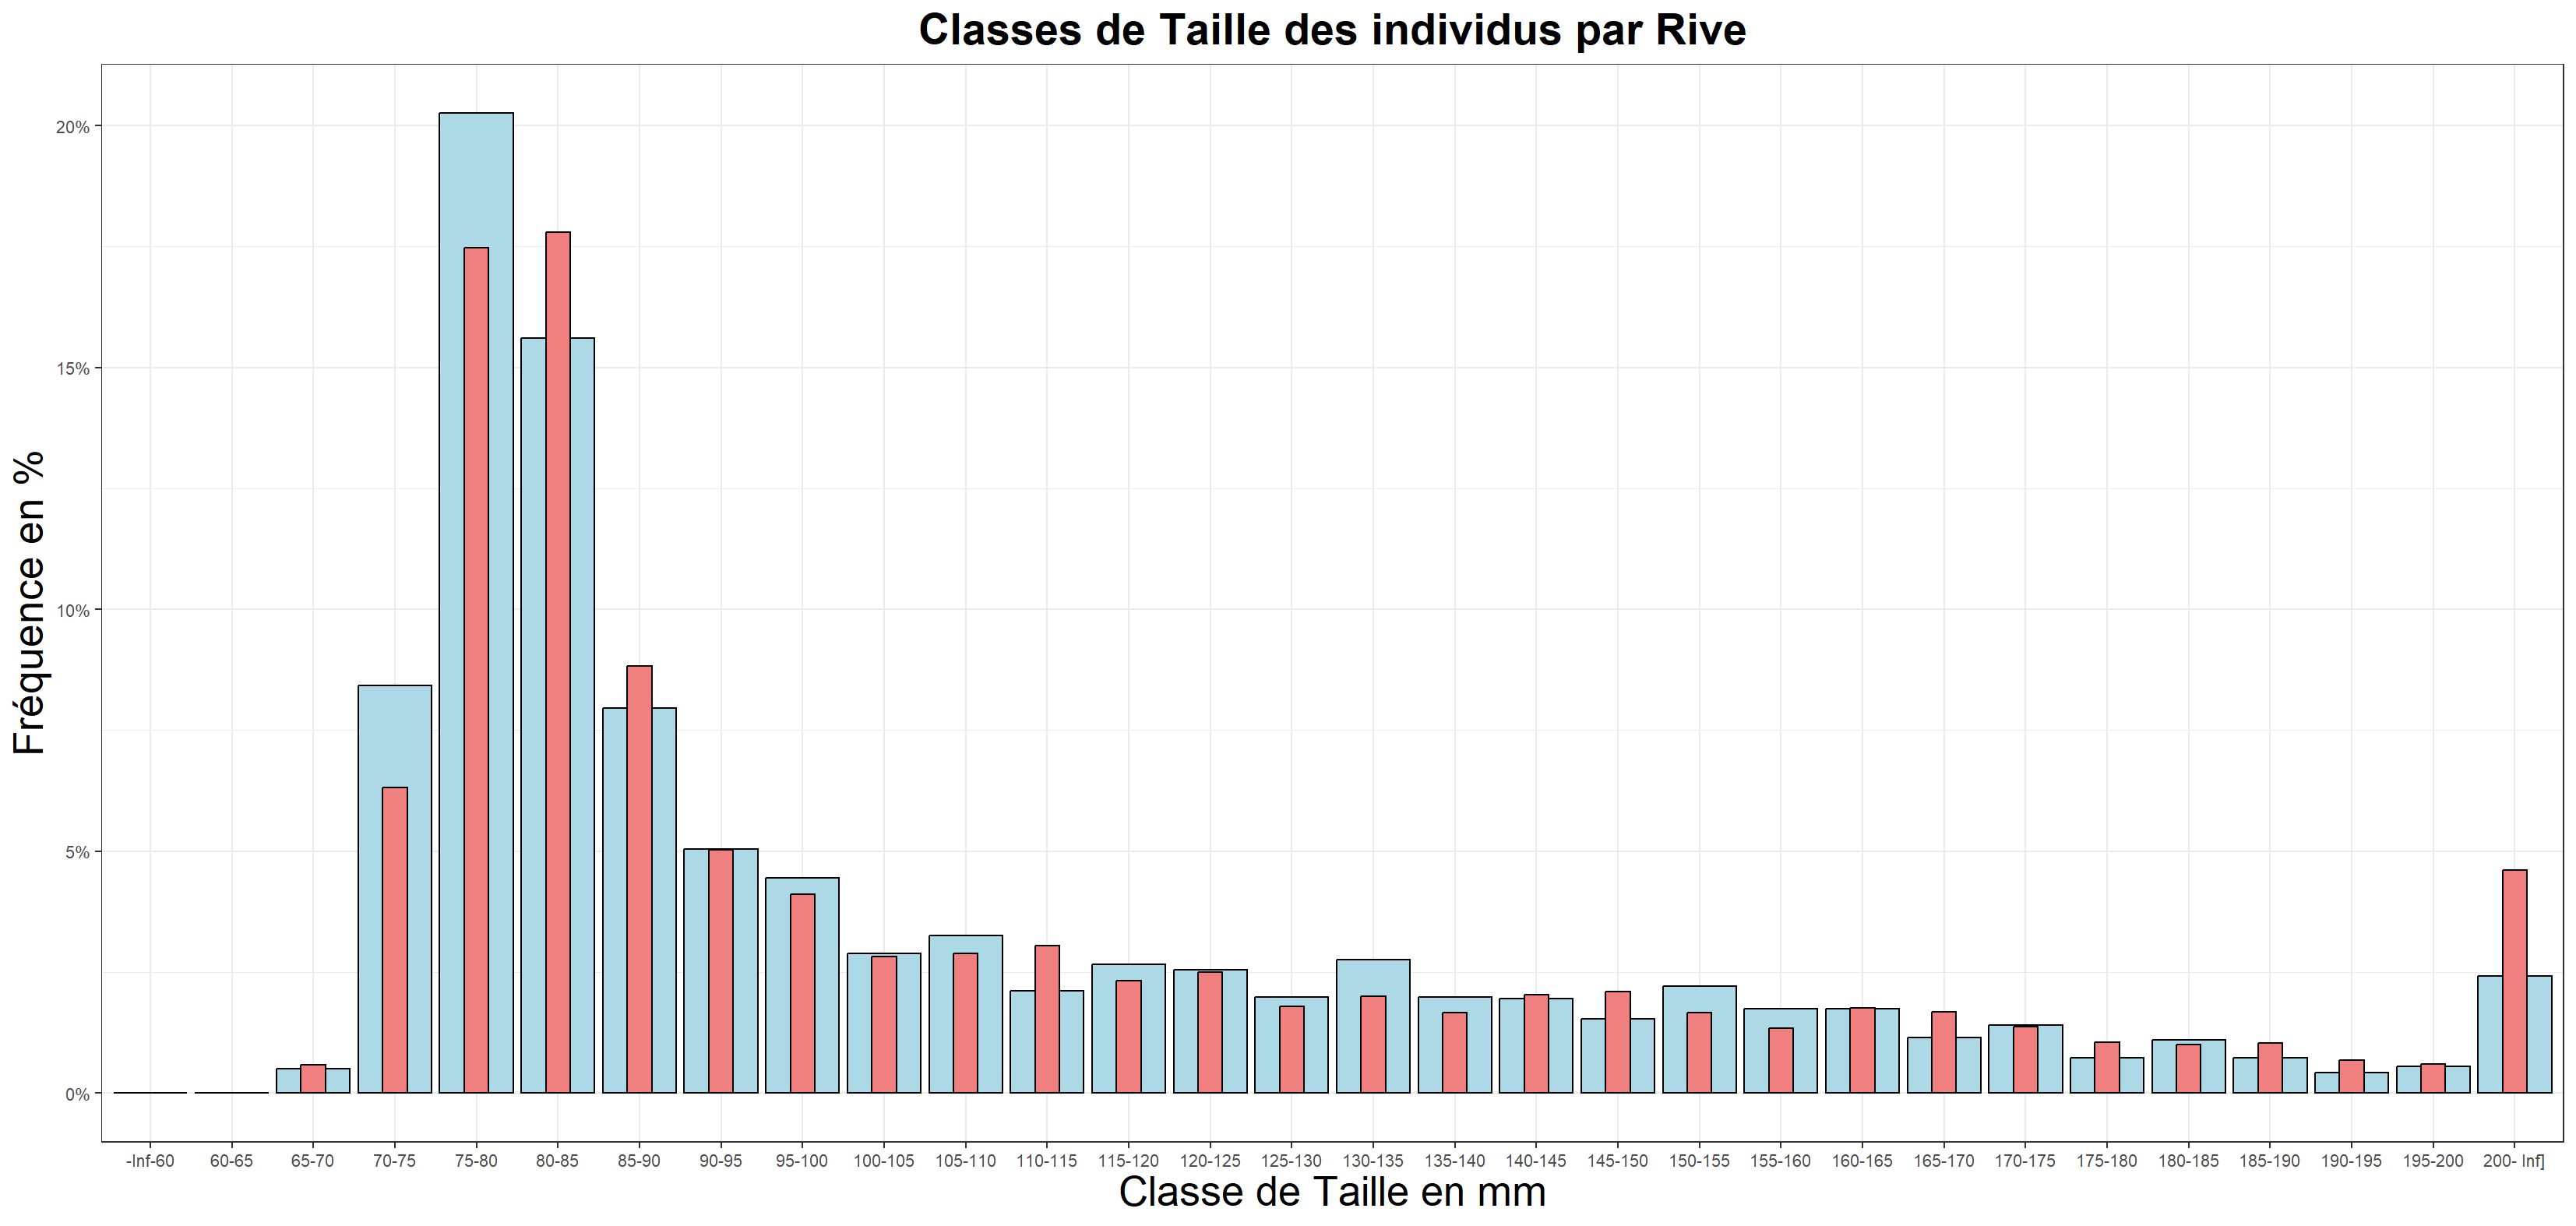
\includegraphics[width=\textwidth]{classe_taille_oral.png}
\caption{Fréquences des classes de tailles (par 5 mm) des anguilles en RG (bleu) et en RD (rouge) en 2024.}
\label{classe_taille_oral}
\end{figure}

\subsubsection{Tailles mensuelles}

Lors des relevés des pièges en début de saison les individus sont des anguilles en reprise de migration c’est à dire des anguilles ayant déjà au minimum plus d’un an. Au fur et à mesure de la saison, les anguilles de l’année commencent à arriver et prédominent durant les mois d’été. De ce fait, la taille mensuelle des anguilles (RG + RD) diminue significativement (Kruskal- test, p < 0,05) comme le montre la (Figure \ref{taille_mois_oral}). Les tests affirment que tous les mois sont statistiquement différents entre eux (hormis avril et mai), ce qui témoigne d’une baisse constante de la taille au fur et à mesure des mois d’avril à août.


\begin{figure}[htpb]
\centering
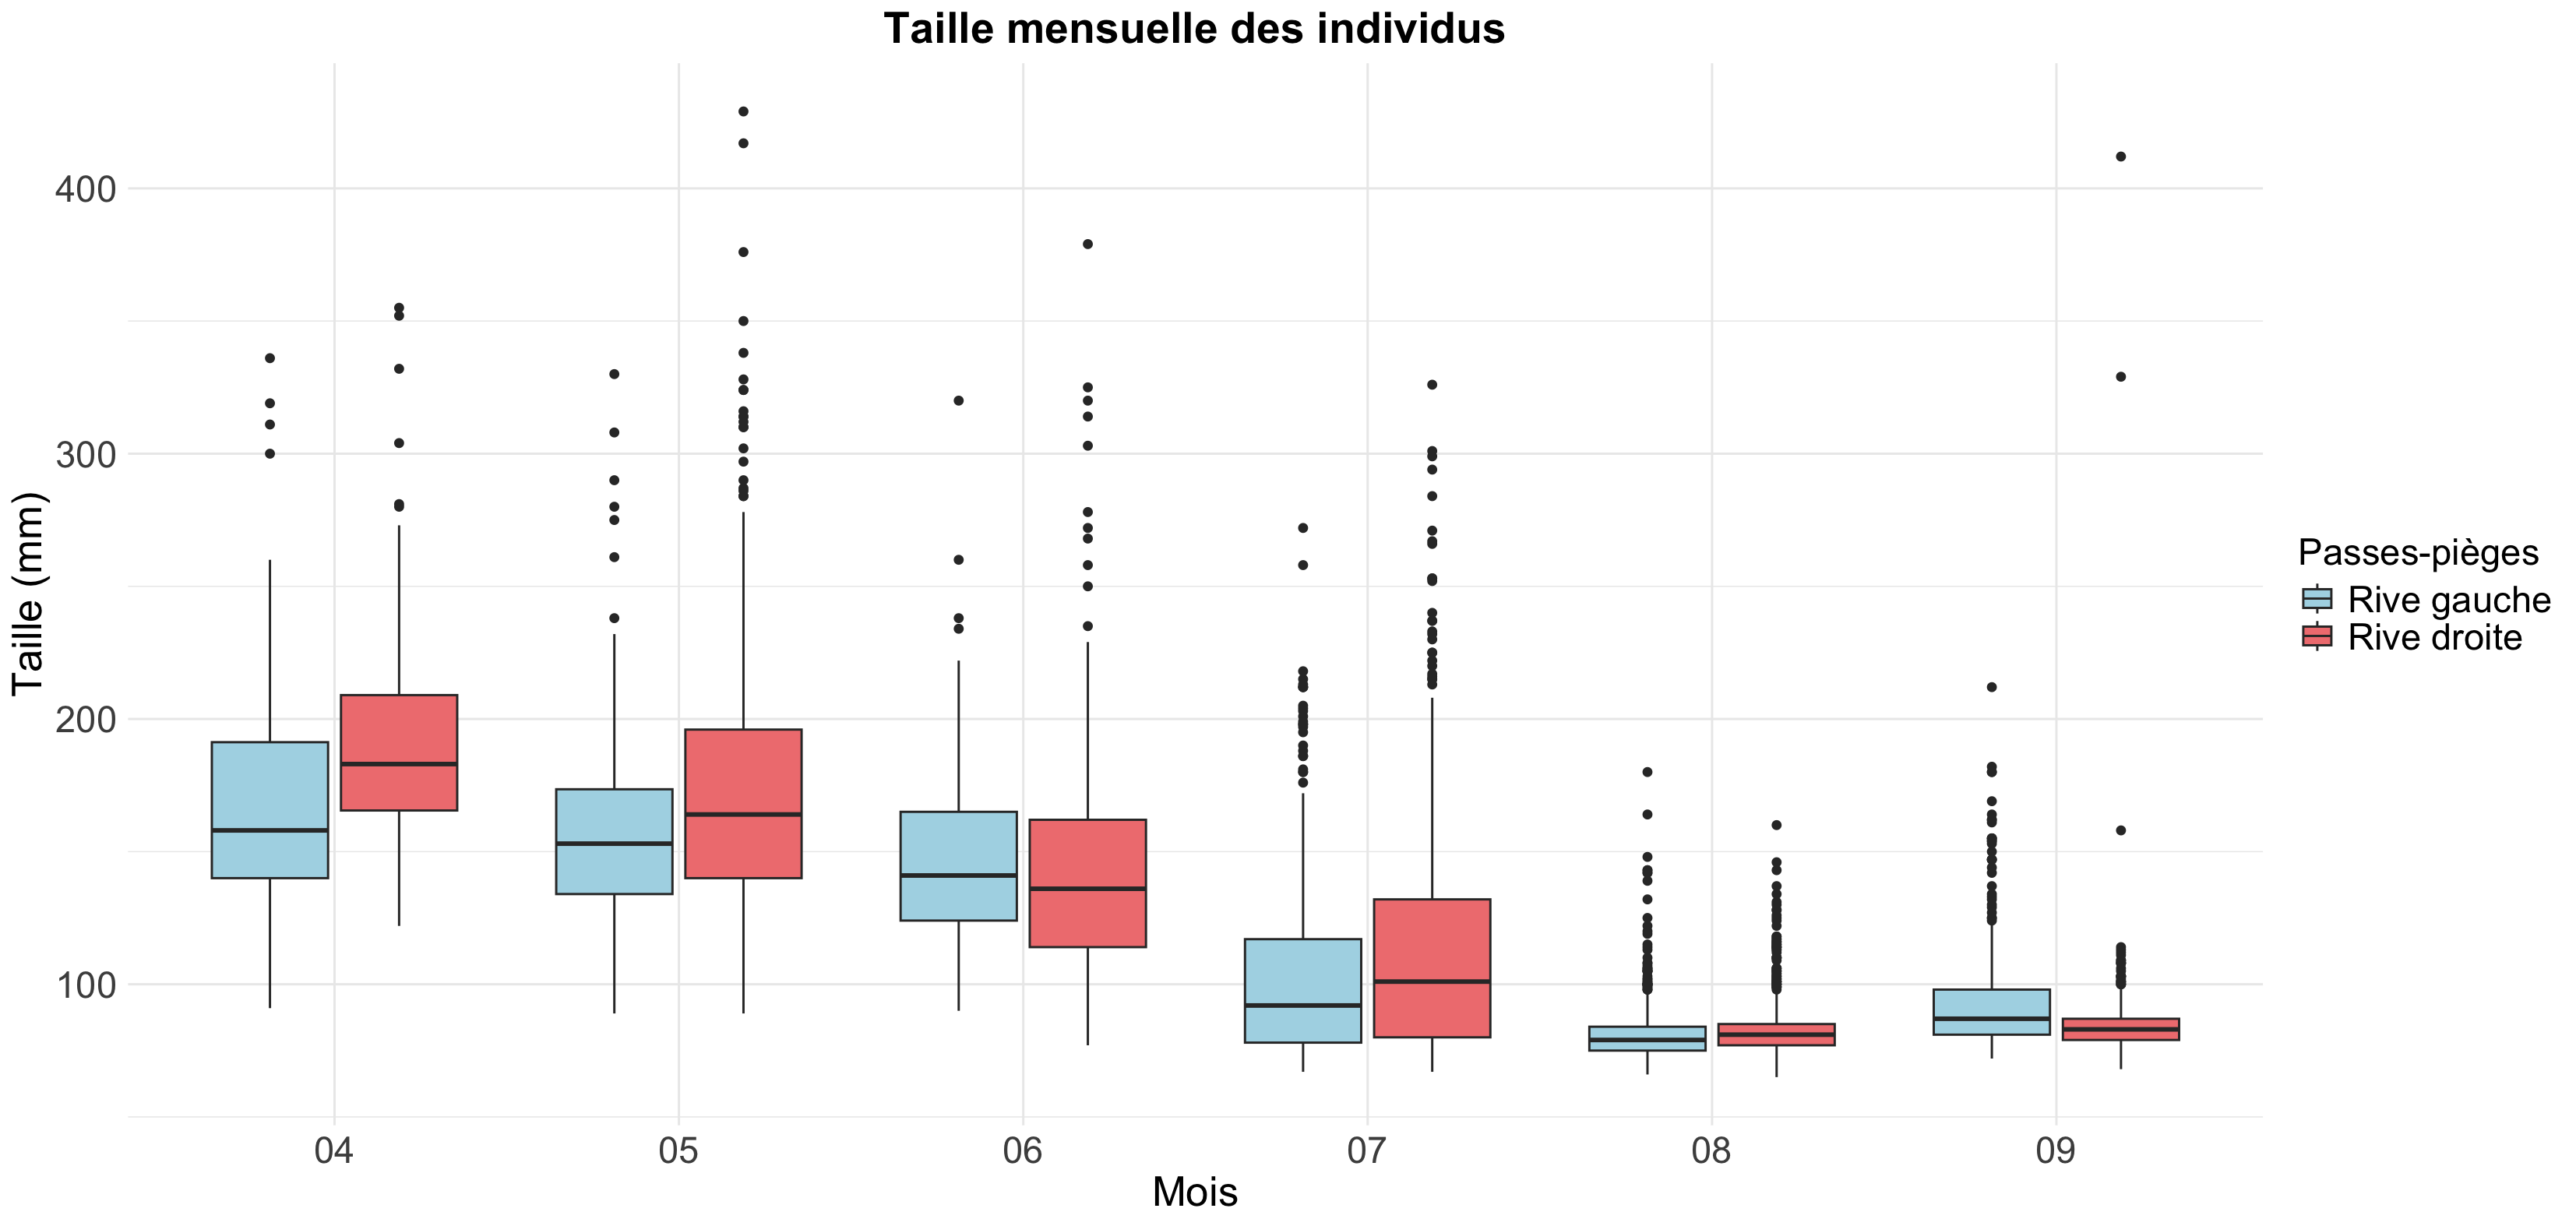
\includegraphics[width=\textwidth]{taille_mois_oral.png}
\caption{Taille (mm) mensuelle des anguilles selon les rives en 2024}
\label{taille_mois_oral}
\end{figure} 

A noter que pour le mois d’août il y a peu de variabilité de taille entre les rives en raison de l’arrivée massive des individus de l’année. 

\subsection{État sanitaire du recrutement 2024}

Cette année encore tous les individus biométrés ont fait l’objet de vérification de présence ou d’absence de pathologies de types anatomo-morphologiques externes ou de types ectoparasites. Chaque pathologie rencontrée possède une codification, à cela est ajouté un code allant de 0 à 4 qui quantifie le nombre de lésion ou le taux de recouvrement des parasites externes ainsi qu’une localisation sur l’individus. Le Tableau \ref{tableau 3} résume les calculs d’indice pathologique (IpG) et parasitaire (IpP) et la condition des anguilles en Seine au barrage de Poses. Au total, 10,6\% des anguilles biométrés (474/4469) présentent des pathologies. Le calcul d’IpG montre une condition des poissons \og Bonne \fg{} et le calcul d’IpP montre une condition des poissons \og excellente \fg{}.  Les pathologies le plus souvent retrouvées sur les anguilles sont les lésions majeures avec 59\% puis 14\% de lésions mineurs et 7\% de parasitisme.

\begin{table}[h!]
\centering
\begin{tabular}{|c|c|c|c|} 
\hline
  & RG  & RD & RG+RD\\ [0.5ex] 
 \hline
 Nombres de poissons examinés & 1758 & 2711  & 4469 \\ 
 \hline
 Nombres de poissons avec pathologies  & 169  & 305  & 474 \\
 \hline
 IpG & \textcolor{green}{0.14} & \textcolor{yellow}{0.21} & \textcolor{green}{0.18}\\
 Condition des poissons & Bonne &  Précaire  & Bonne\\
 \hline
 IpP & \textcolor{blue}{0.03} & \textcolor{blue}{0.03} & \textcolor{blue}{0.03}\\ [0.5ex] 
 Condition des poissons & Excellente & Excellente  & Excellente\\
 \hline
 Parasitisme & 32\%  & 24\% & 27\%\\
 Lésions majeures & 49\%  & 65\% & 59\%\\
 Lésions mineures  & 19\% &  11\%  & 14\%\\ [1ex] 
 \hline
 
\end{tabular}
\caption{Synthèse de l’état sanitaire du recrutement 2024}
\label{tableau 3}
\end{table}


Si l’on traite la rive droite et la rive gauche séparément les calculs des indices pathologiques montrent une condition des poissons \og bonne \fg{} pour la rive gauche et \og précaire \fg{} pour la rive droite. Les calculs d’indice parasitaire donnent les mêmes résultats que pour les deux rives confondues avec une condition des poissons \og excellente \fg{} à la fois en rive gauche et en rive droite. La distribution des catégories pathologiques est assez similaire avec seulement un pourcentage de parasitisme plus élevé en rive gauche avec 32\% et un pourcentage de lésions majeures plus faibles avec 49\%. 

La (Figure \ref{patho}) est une synthèse des pathologies ainsi que des intensités lésionnelles observées sur les deux rives confondues. Au total 11 pathologies ont été observées sur les anguilles dont 2 issues de parasites, les points noirs et les points blancs. La pathologie la plus représentée est la présence de marques d’érosion (50\%) sur les individus. Ensuite, la présence de points noirs est retrouvée à 18.2\% et la présence de plaie avec un pourcentage de 12.3\%.

\begin{figure}[htpb]
\centering
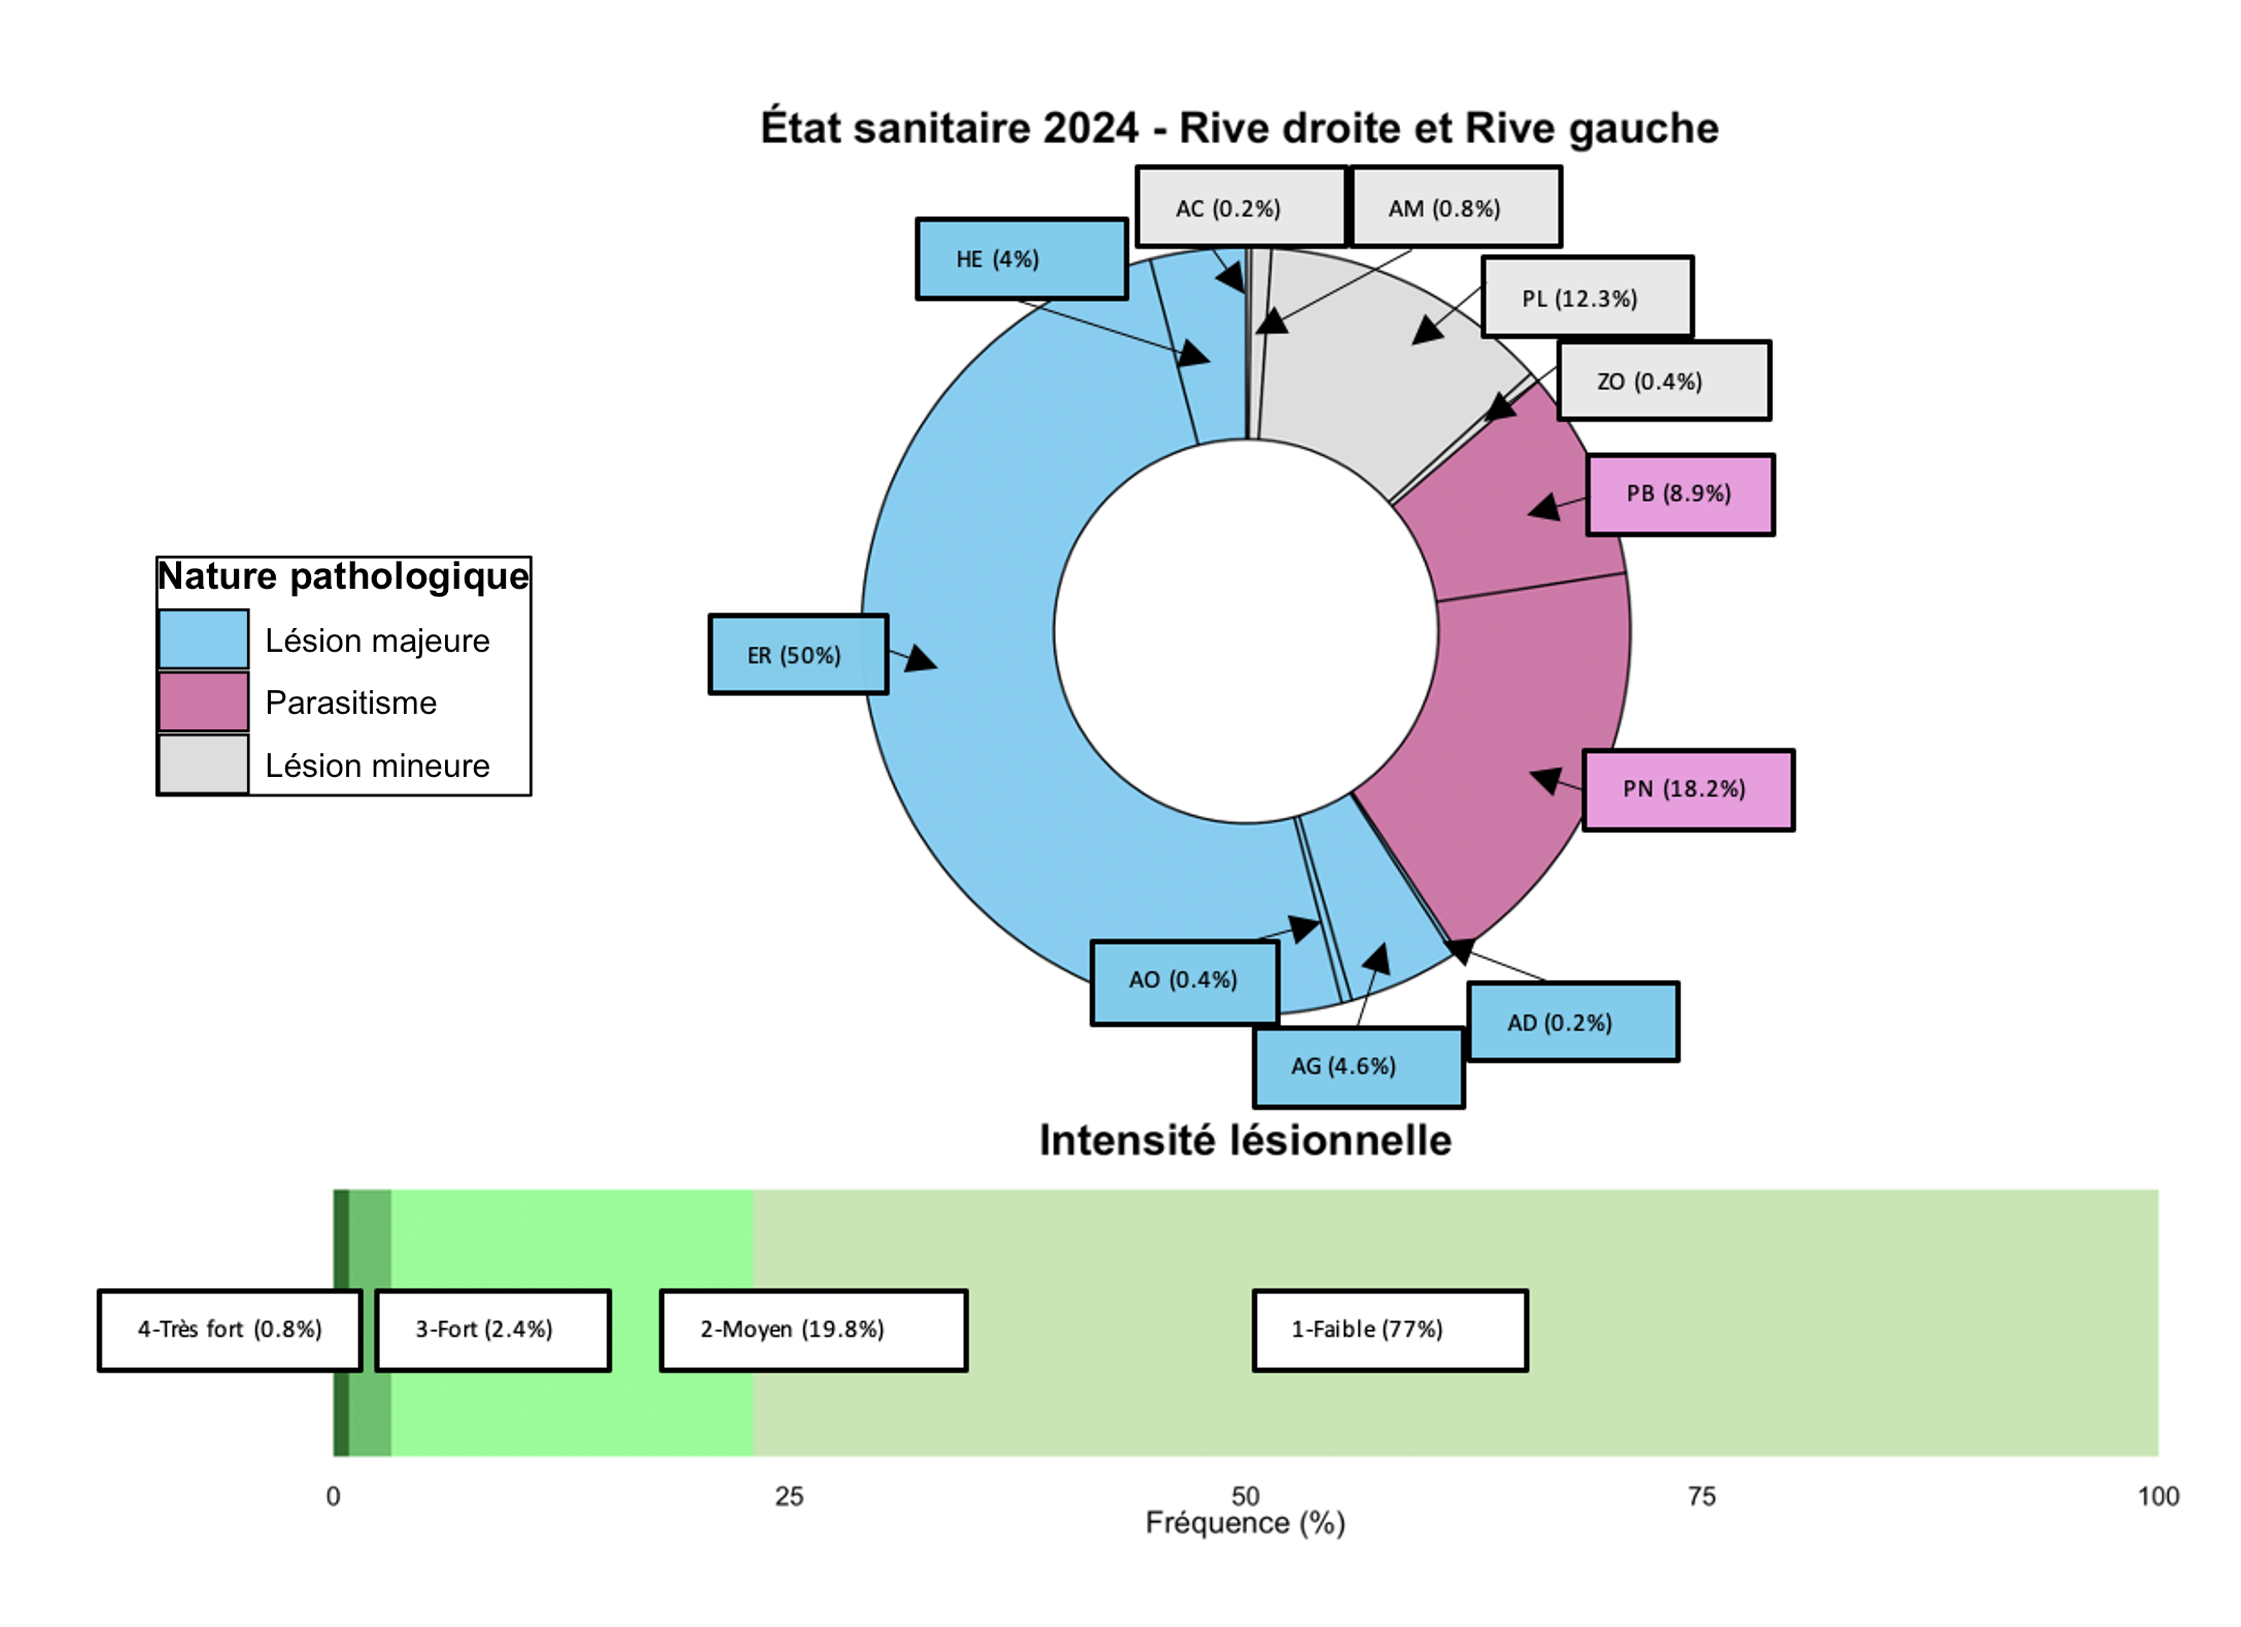
\includegraphics[width=0.5\textwidth]{patho.png}
\caption{Synthèse des pathologies et des intensités lésionnelles observés en rive droite et rive gauche. PN=Points noirs / PB=Points blancs / AG=Grosseurs-Tumeurs / AO=Absence d’organes / ER=Érosion / HE=Hémorragie / AM=Maigreur / PL=Plaies / AC=Altération de la couleur / AD=Difformité / ZO=État pathologique multiforme.}
\label{patho}
\end{figure} 


\subsection{Influence des facteurs environnementaux }

L’influence des paramètres environnementaux sur les effectifs de captures des anguilles est représentée par la (Figure \ref{ACP}). Le pourcentage d’inertie total des deux dimensions est satisfaisant avec 82,3\%. Toutes les variables sont fortement représentées. Le premier axe est très représenté par les variables Température de l’eau, Température de l’air et Débit. Le second axe est lui très représenté par la variable Coefficient de marée. La température de l’eau et la température de l’air sont fortement corrélées positivement entre elles. Avec une projection des individus sur ce graphique, nous pouvons voir qu’en début de saison les fortes valeurs de débit exercent une influence négative sur les effectifs des anguilles (Figure \ref{Individus}). En effet, le mois d’avril est significativement différent des autres mois, le débit était élevé et les captures faibles. Puis au fur et à mesure de la saison, les températures ont augmenté tout comme les captures. Cette année le débit était largement supérieur au débit moyen des années précédentes. Le mois d’avril 2024 est le mois avec des valeurs de débit le plus élevé depuis 2014 (Figure \ref{graph_debit_oral}). Le mois de juin ne semble pas être influencé par une variable en particulier. Les mois de juillet et d’août semblent eux influencés par la température de l’air et la température de l’eau. Ces deux mois représentent quasiment la totalité des anguilles capturées sur la période du suivi.

\begin{figure}[htpb]
\centering
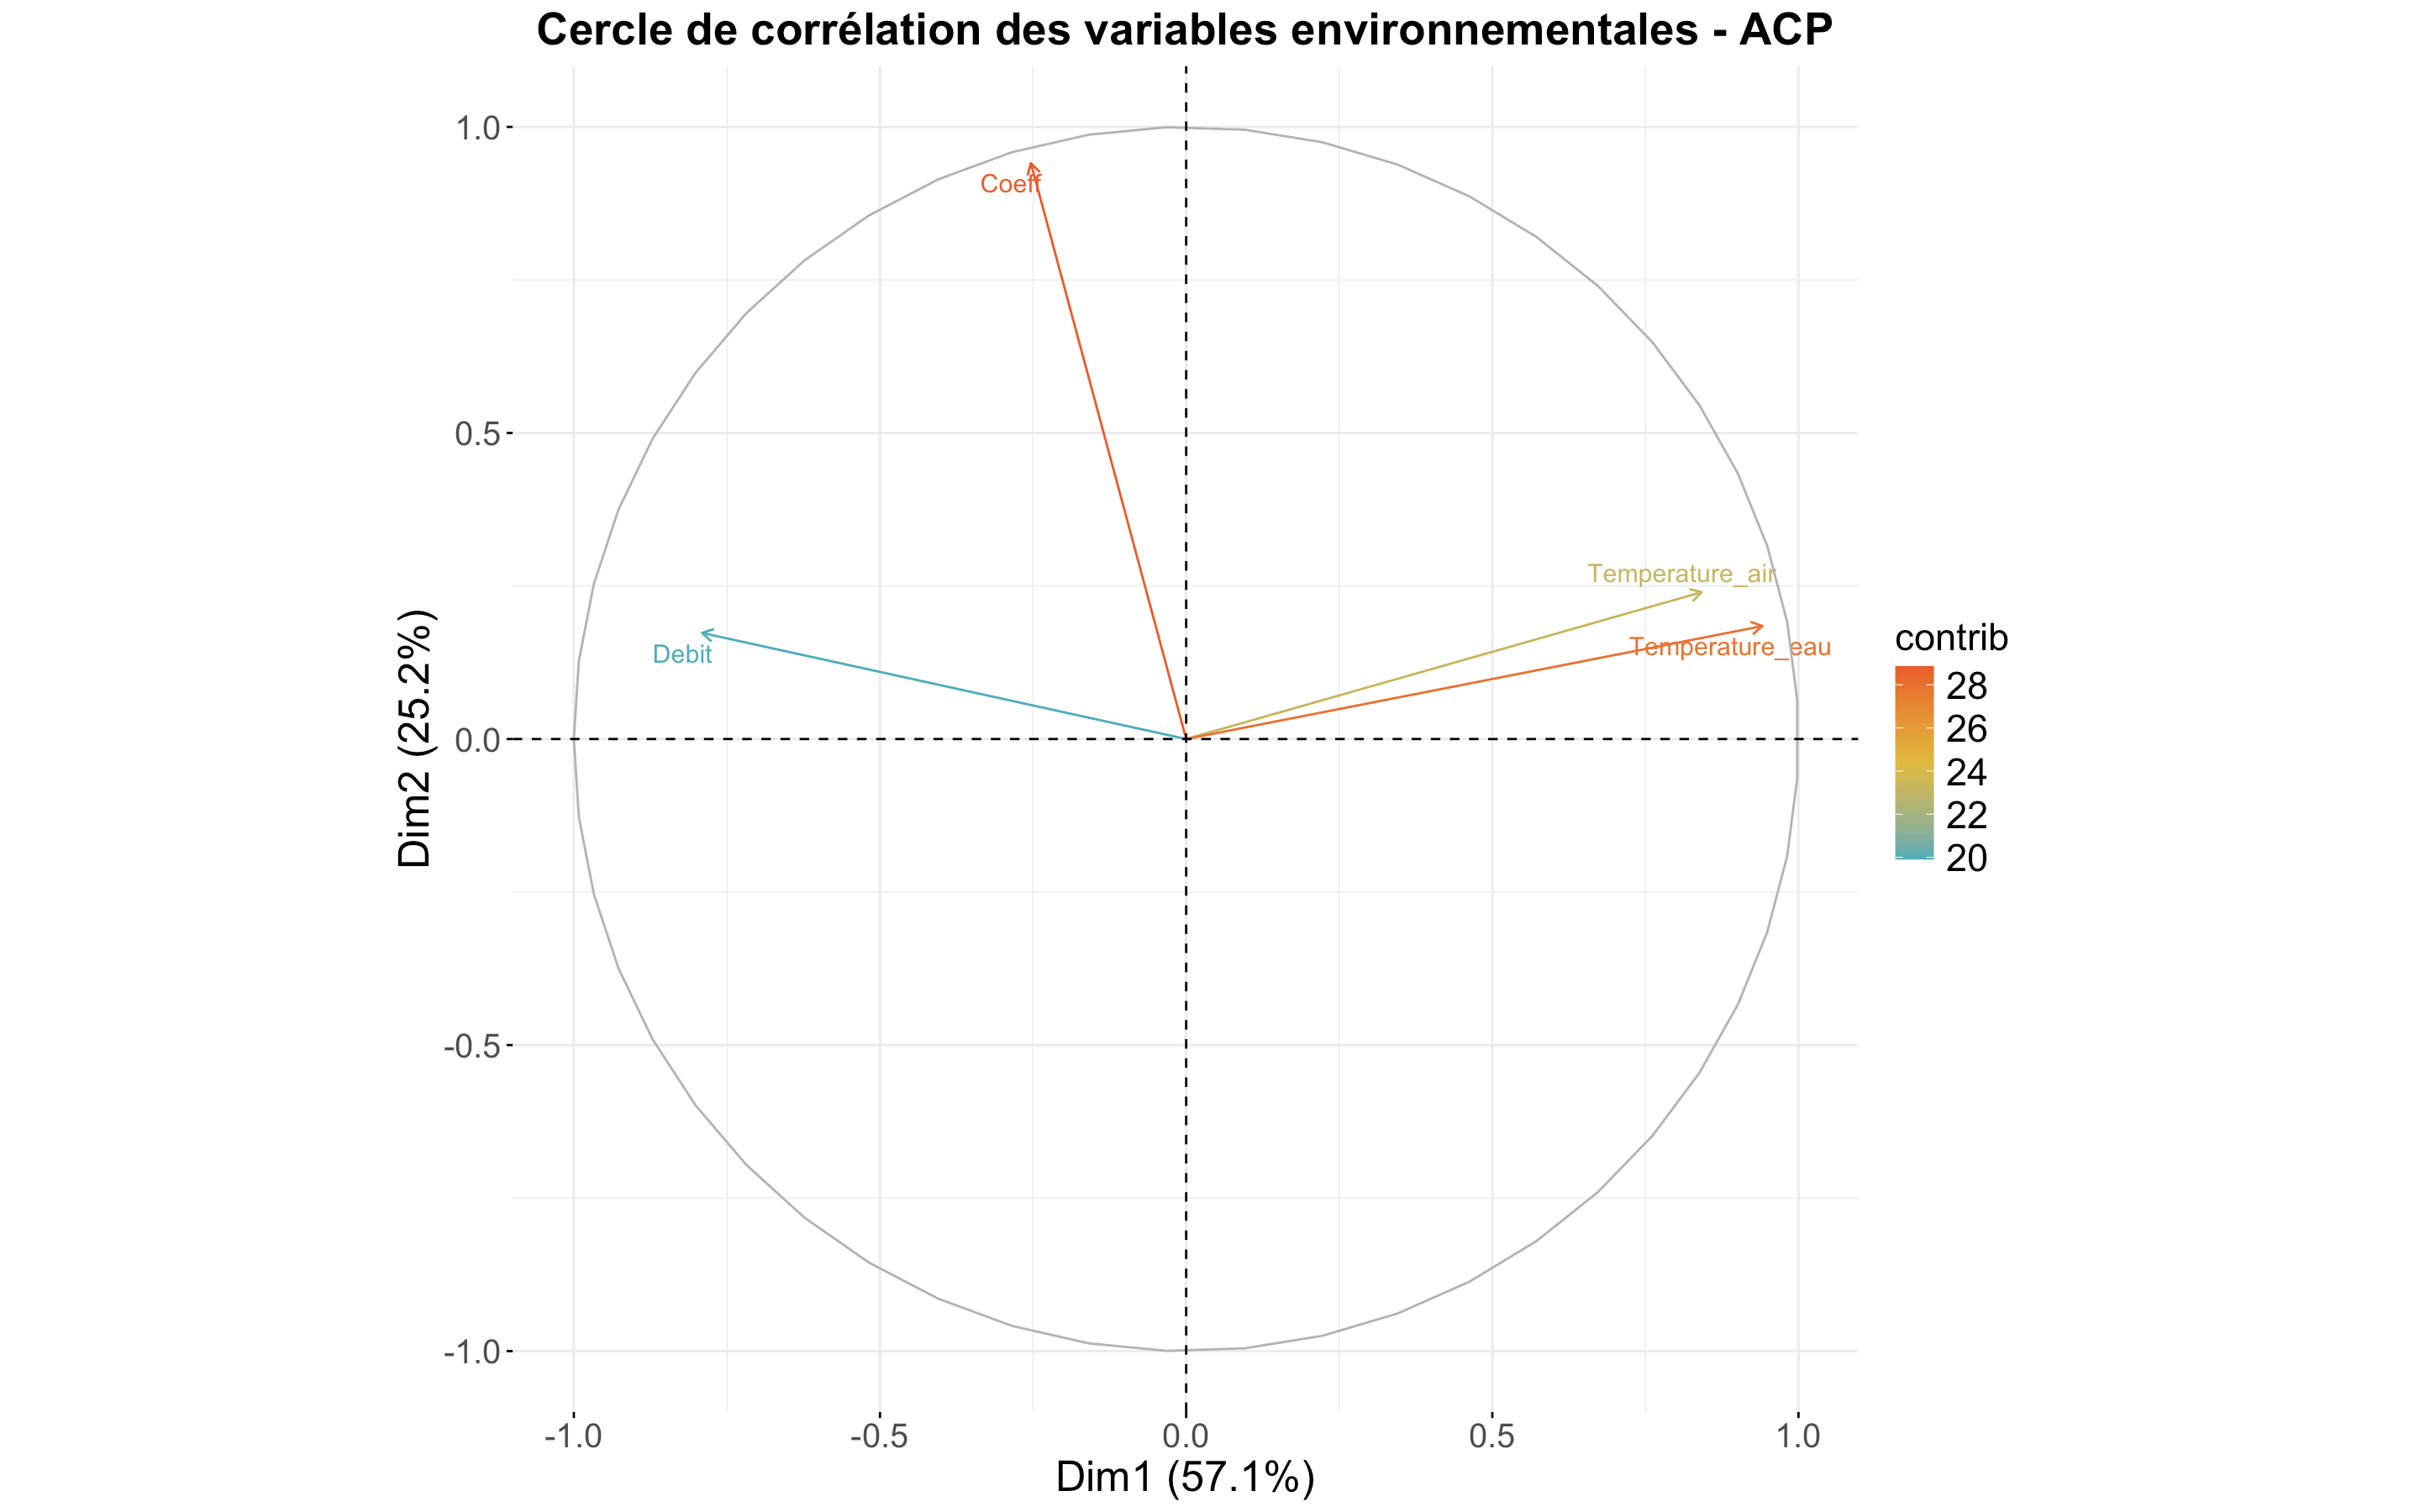
\includegraphics[width=\textwidth]{ACP.png}
\caption{Cercle de corrélation des variables environnementales – ACP}
\label{ACP}
\end{figure} 


\begin{figure}[htpb]
\centering
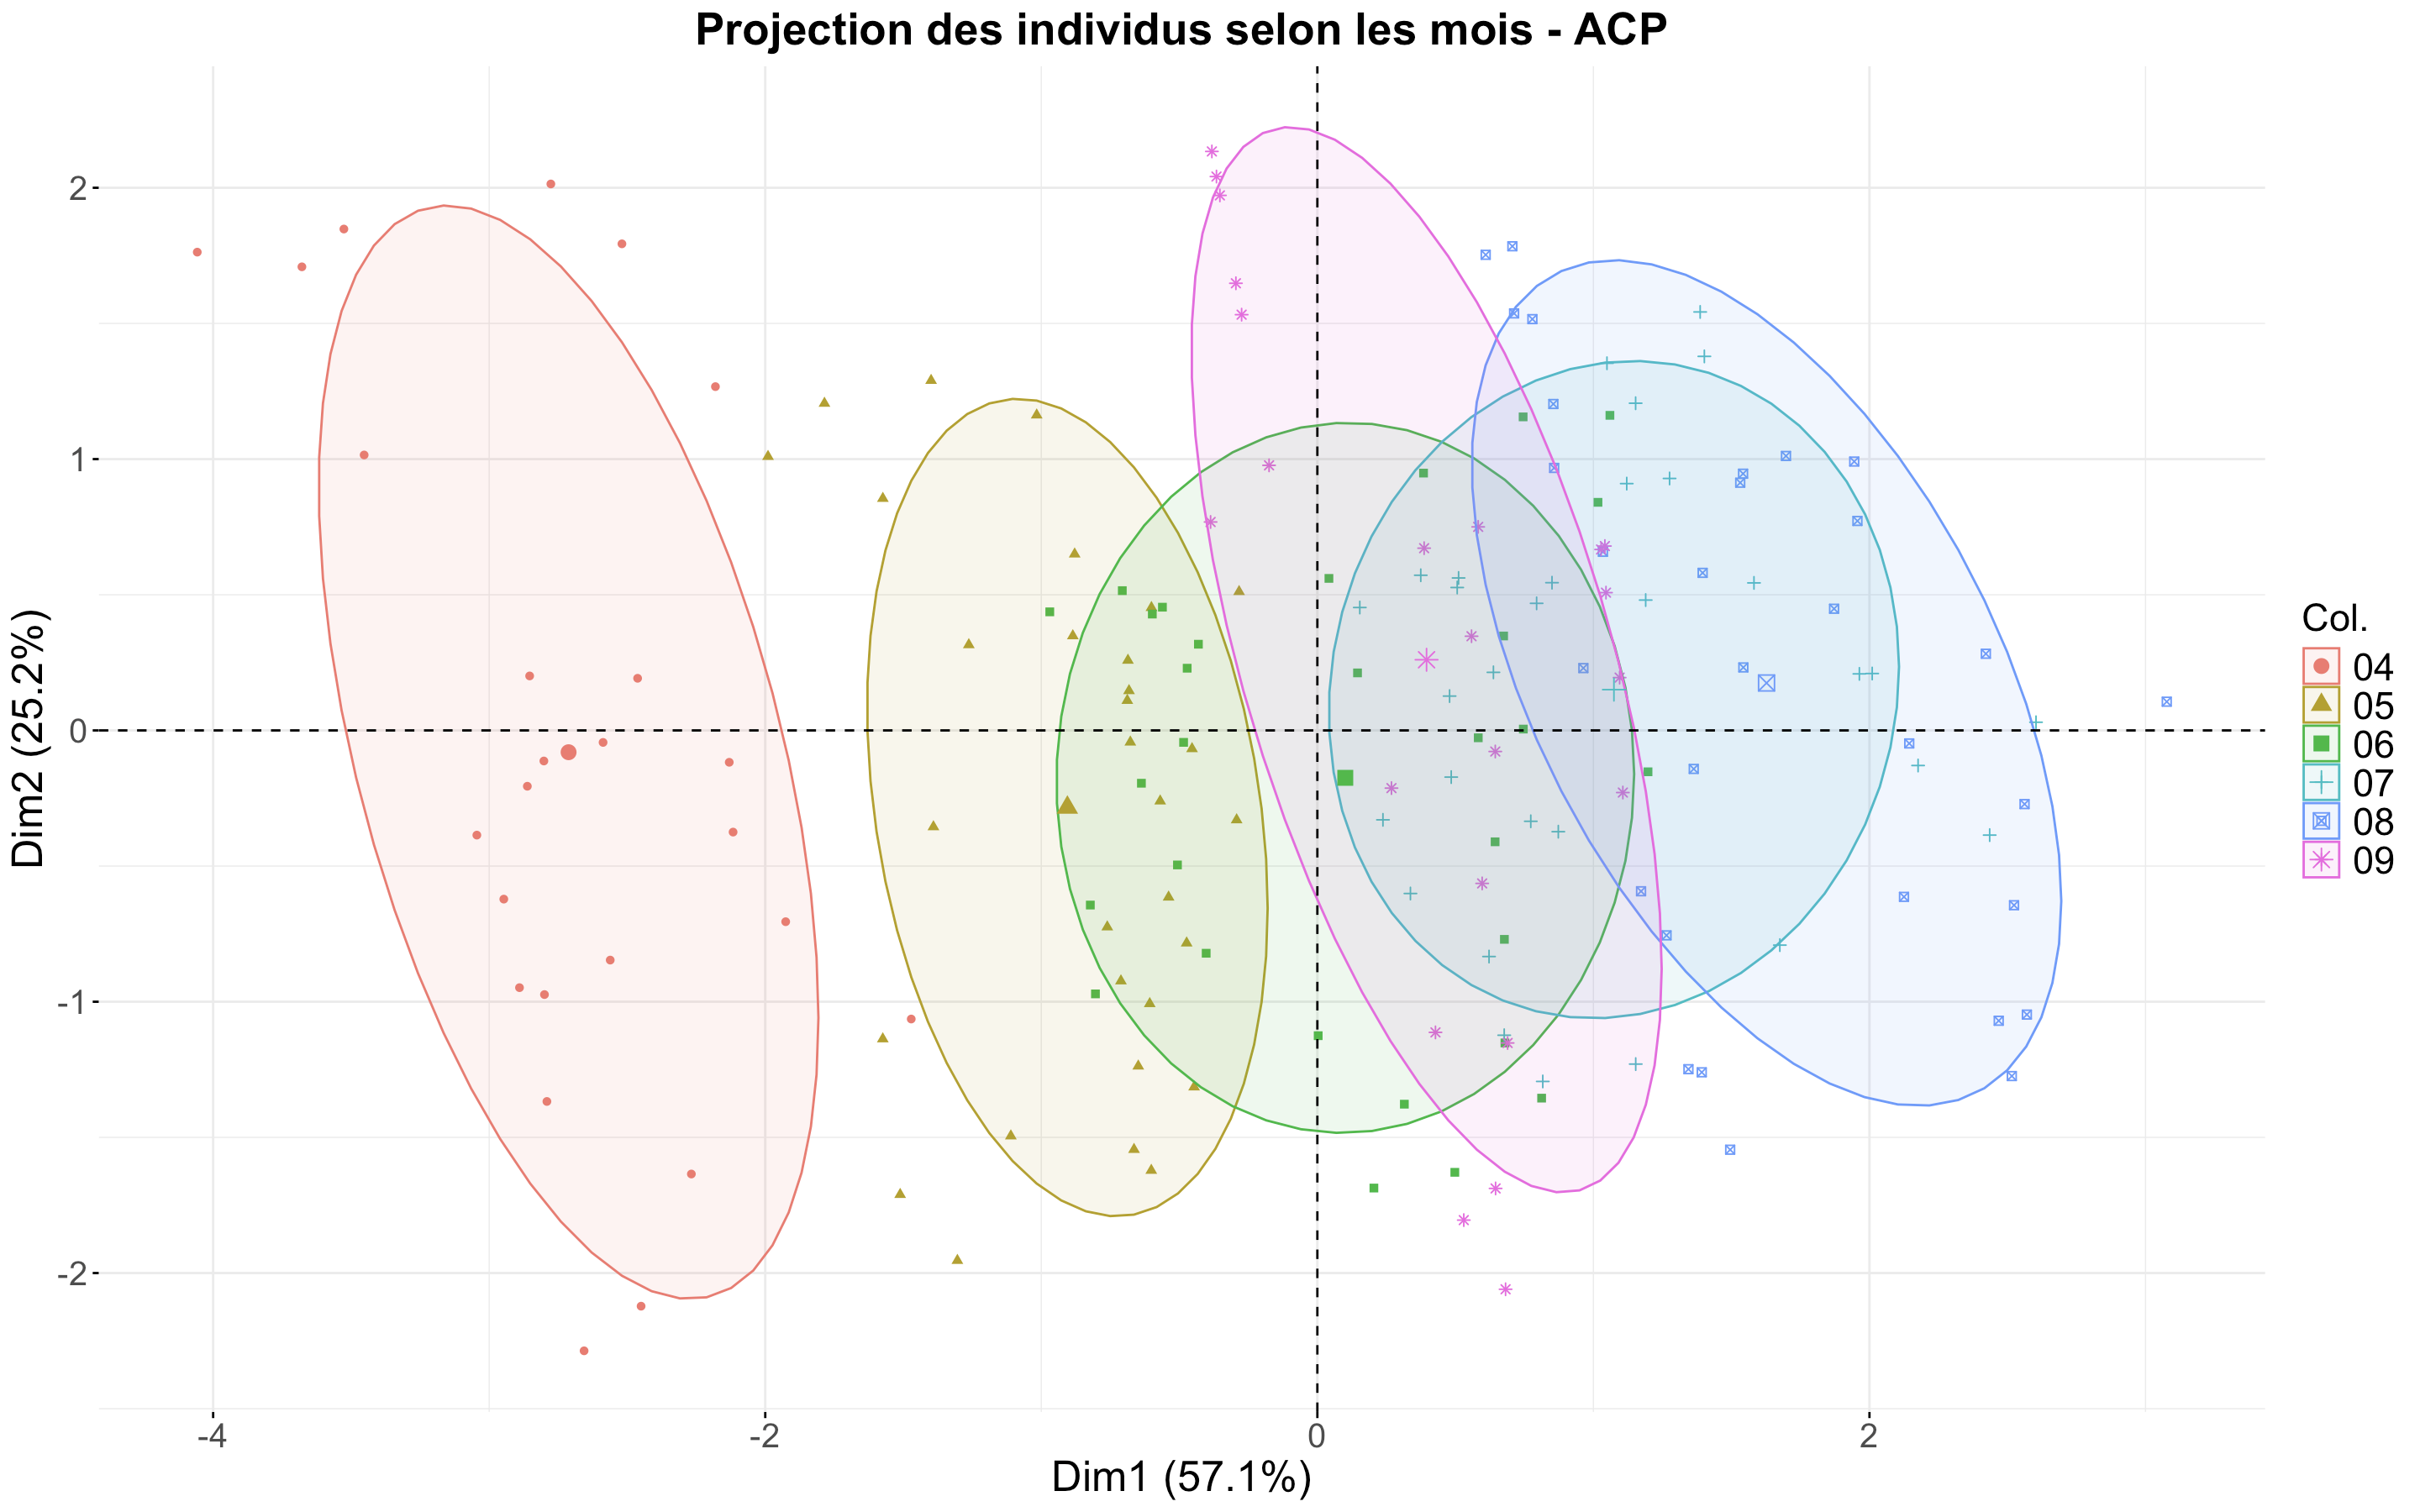
\includegraphics[width=\textwidth]{Individus.png}
\caption{Projection des individus selon les variables environnementales par mois de captures (ACP)}
\label{Individus}
\end{figure} 

\begin{figure}[htpb]
\centering
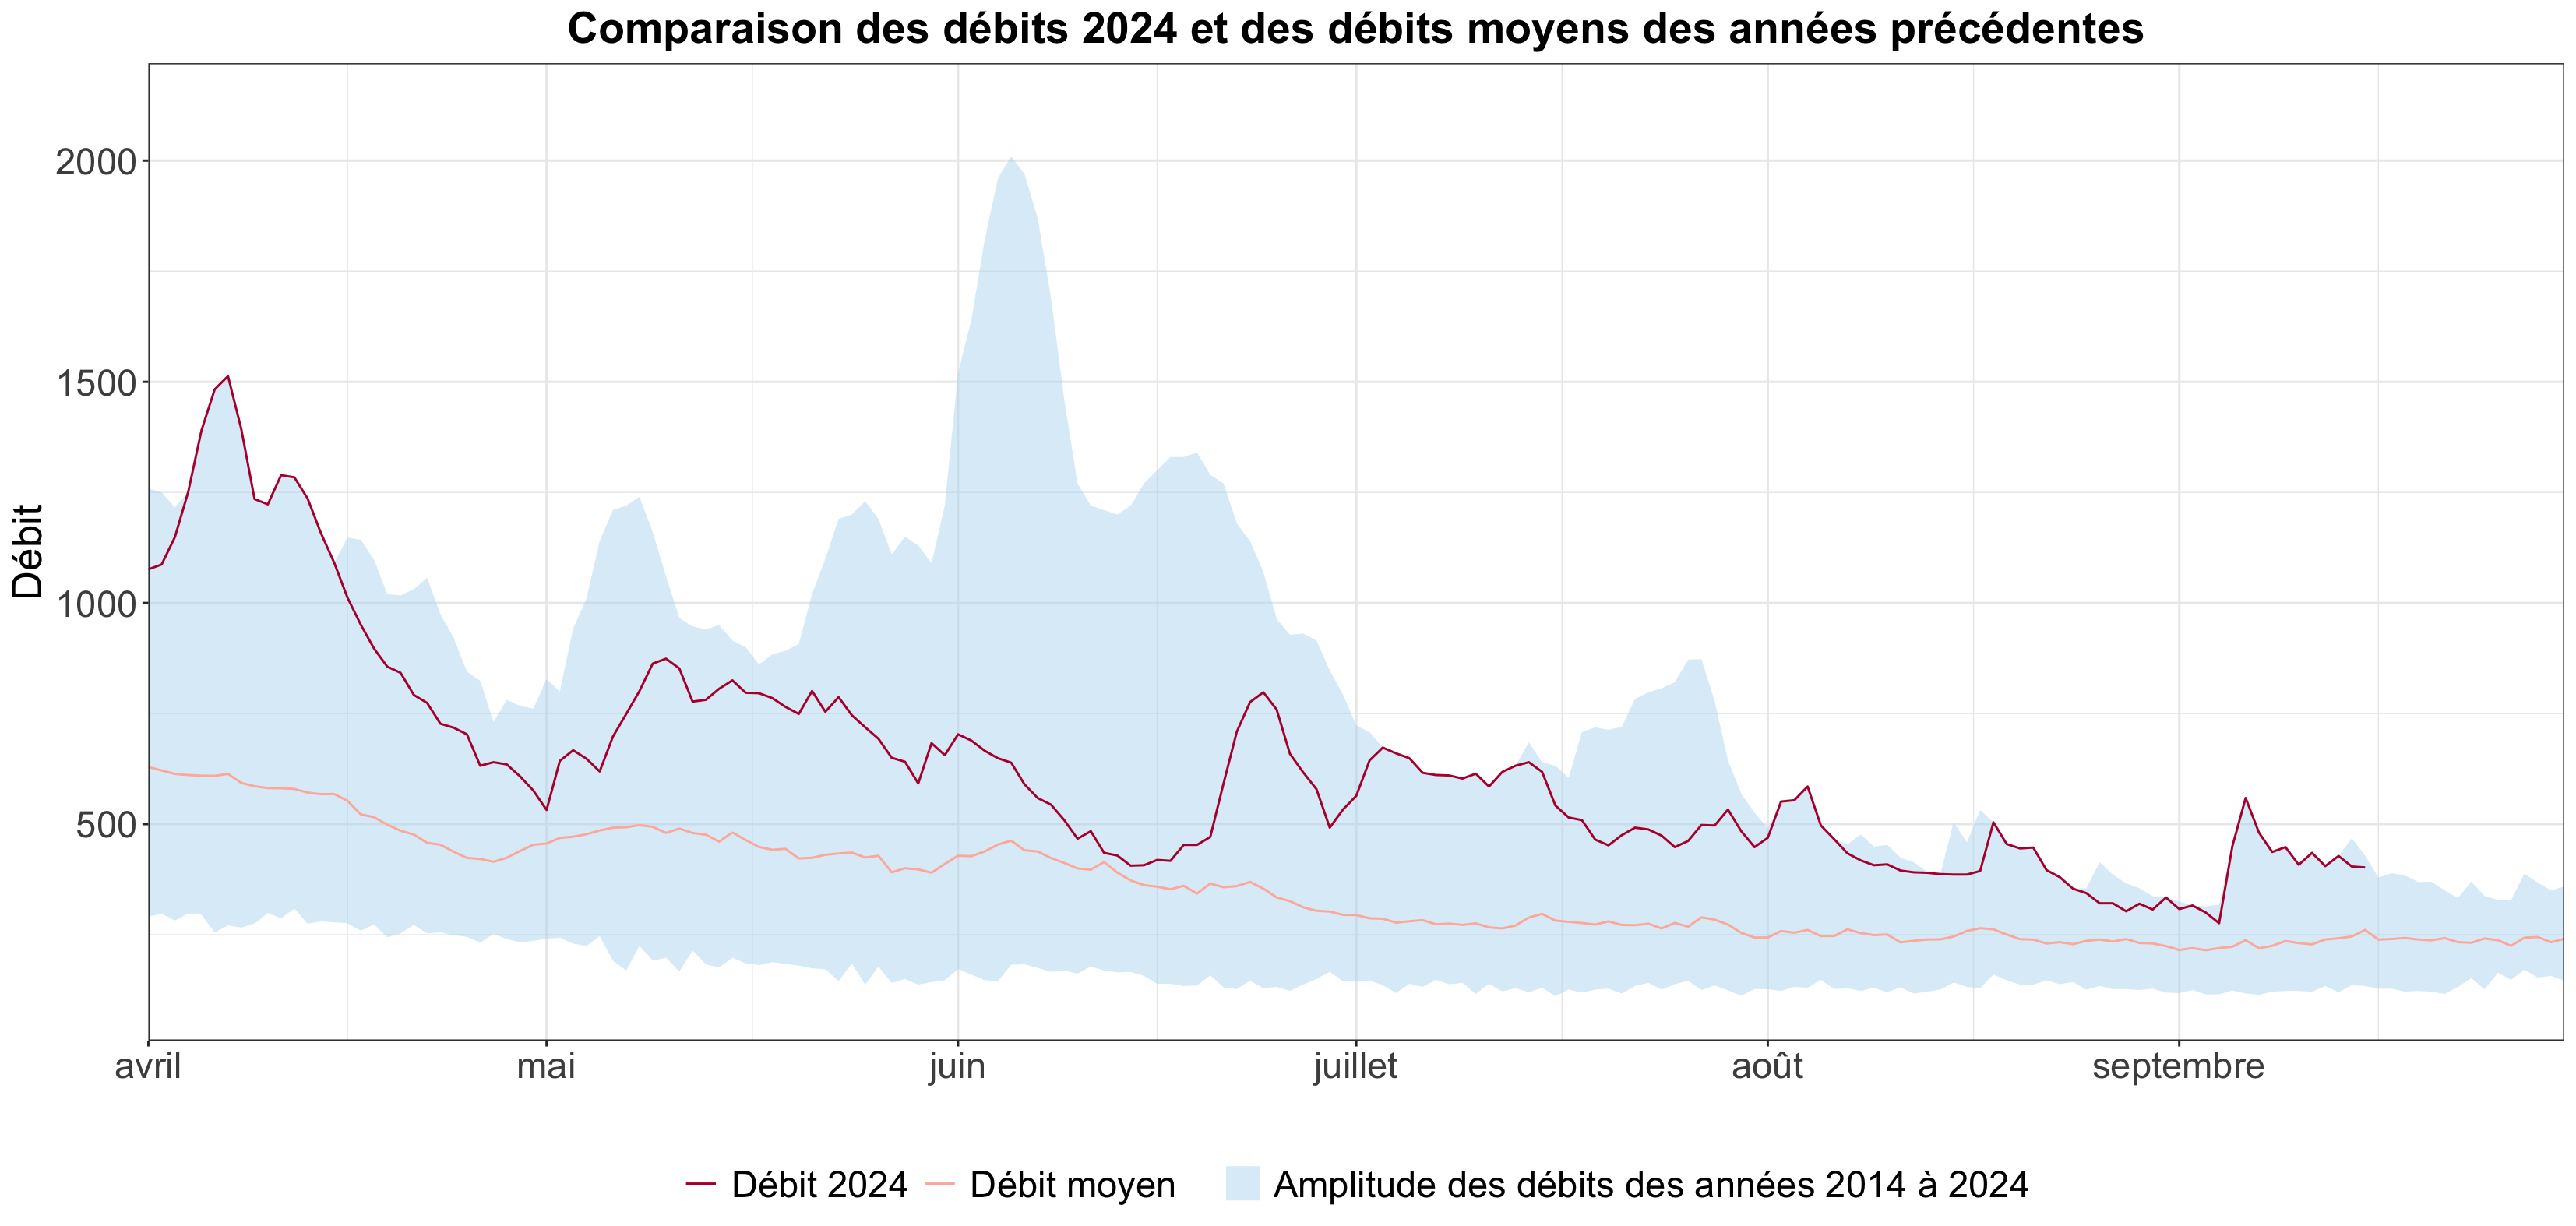
\includegraphics[width=\textwidth]{graph_debit_oral.png}
\caption{Comparaison des débits de 2024 et des débits moyens des années précédentes}
\label{graph_debit_oral}
\end{figure} 

La température de l’air a augmenté début juillet ce qui a entrainé un réchauffement de l’eau de la Seine dépassant les 20°C pour la première fois de la saison, à ce moment-là un premier léger pic de migration des anguilles peut être observé. À la mi-juillet une seconde vague de chaleur plus importante a de nouveau permis à la Seine de dépasser une température de 20°C jusqu’à atteindre début août 23°C (Figure \ref{graph_temp_eau_oral}). Un second pic de migration plus important est observé début août et le pic de migration le plus important est lui observé mi-août avec une température de Seine aux alentours des 23°C.


\begin{figure}[htpb]
\centering
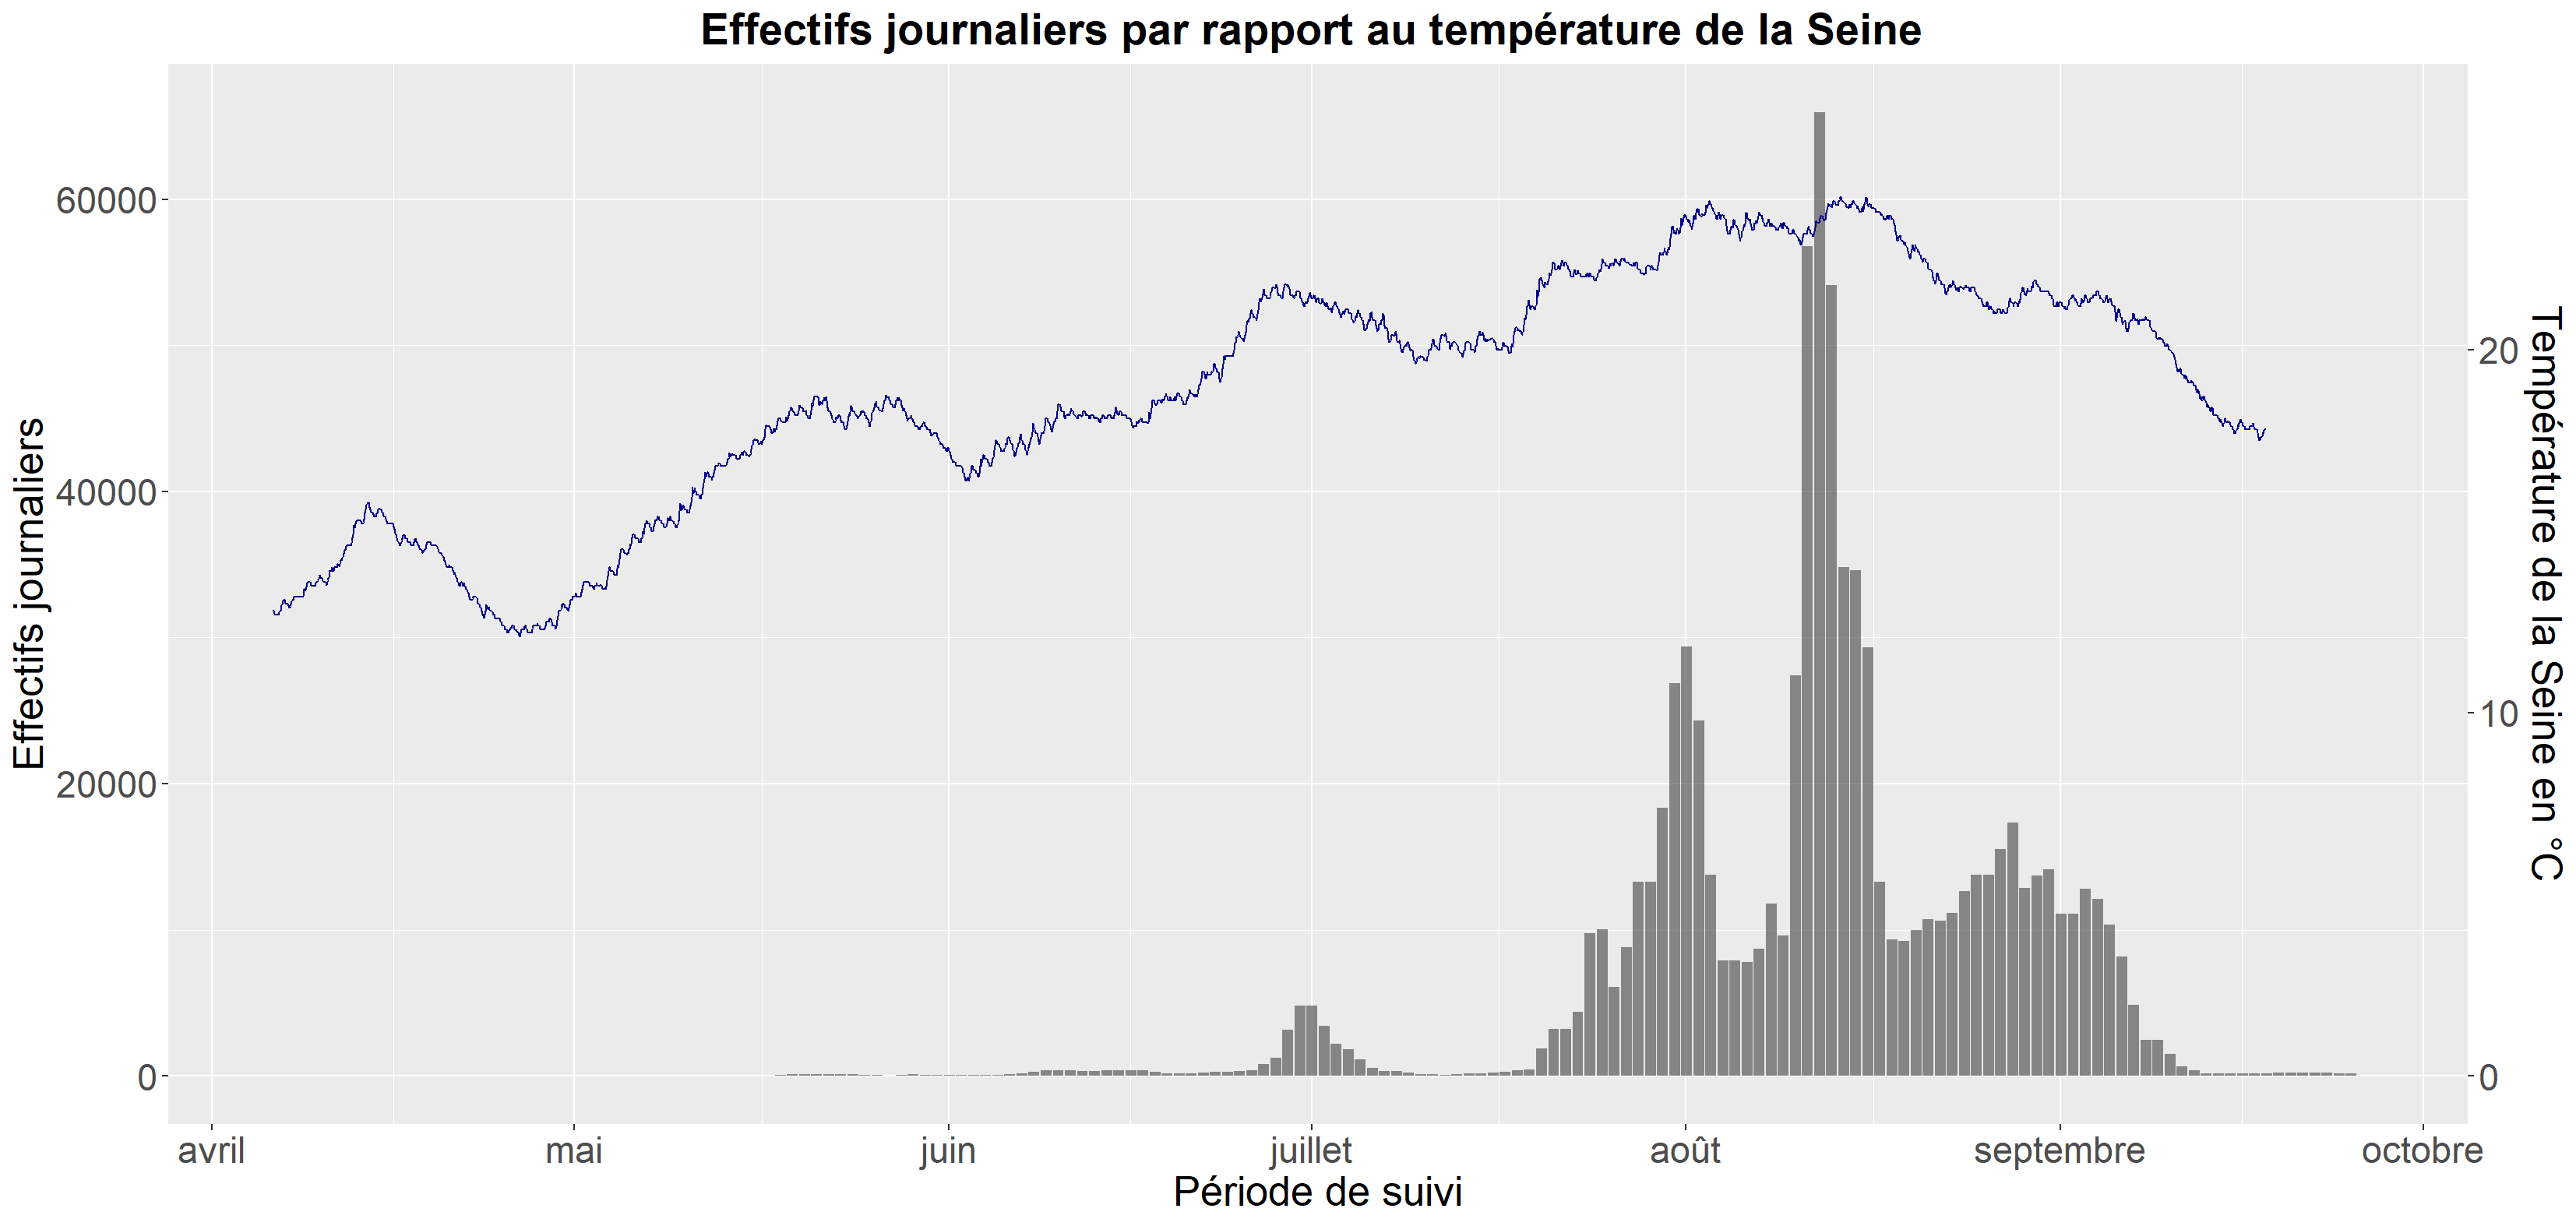
\includegraphics[width=\textwidth]{graph_temp_eau_oral.png}
\caption{Effectifs journaliers selon la température de la Seine (°C) en rive gauche et rive droite confondues en 2024.}
\label{graph_temp_eau_oral}
\end{figure} 

\subsection{Bilan des flottangs }

\subsubsection{Effectifs 2024}


Les deux flottangs mis en place cette année sont en aval de la rampe en rive droite (AVR) et l’autre en aval de la rampe en rive gauche (AVT). Les flottangs ont été mis en place le 29 mai ce qui est plus tard contrairement aux autres années de suivi car le débit et le niveau d’eau étaient trop élevé. Pour l’AVR le premier individu a été observé le 31 mai et pour l’AVT le premier individu a été observé le 3 juin. Dans les flottangs un total de 6702 anguilles ont été piégées, 5006 (70\%) dans le flottang AVR et 1694 (30\%) dans le flottang AVT. La (Figure \ref{graph_flottang_oral}) illustre les effectifs journaliers et cumulés d'anguilles pour les deux flottangs. Pour le flottang AVR, peu d’anguilles ont été piégées jusqu’à la mi-juillet. Un premier pic est observé mi-juillet, un second pic le plus important est observé fin juillet début août et un dernier pic est observé mi-août. Les pics observés sur ce flottang sont les mêmes pics que nous avons observés avec les effectifs d’anguilles piégées en rive droite. La seule différence est que le pic le plus important pour le flottang est fin juillet-début août alors que le pic le plus important en rive droite et à la mi-août. En ce qui concerne le flottang AVT, nous pouvons constater qu’aucune anguille n’est capturée dans le flottang AVT du 10 au 24 juillet, durant cette période le flottang a été bloqué et les relèves étaient impossibles. Pour le flottang AVT, trois pics de captures sont visibles, le premier fin juin-début juillet, le second fin juillet-début août et le troisième le plus important à la mi-août. Ici les pics de captures dans le flottang AVT sont identiques aux pics de migration observés en rive gauche.


\begin{figure}[htpb]
\centering
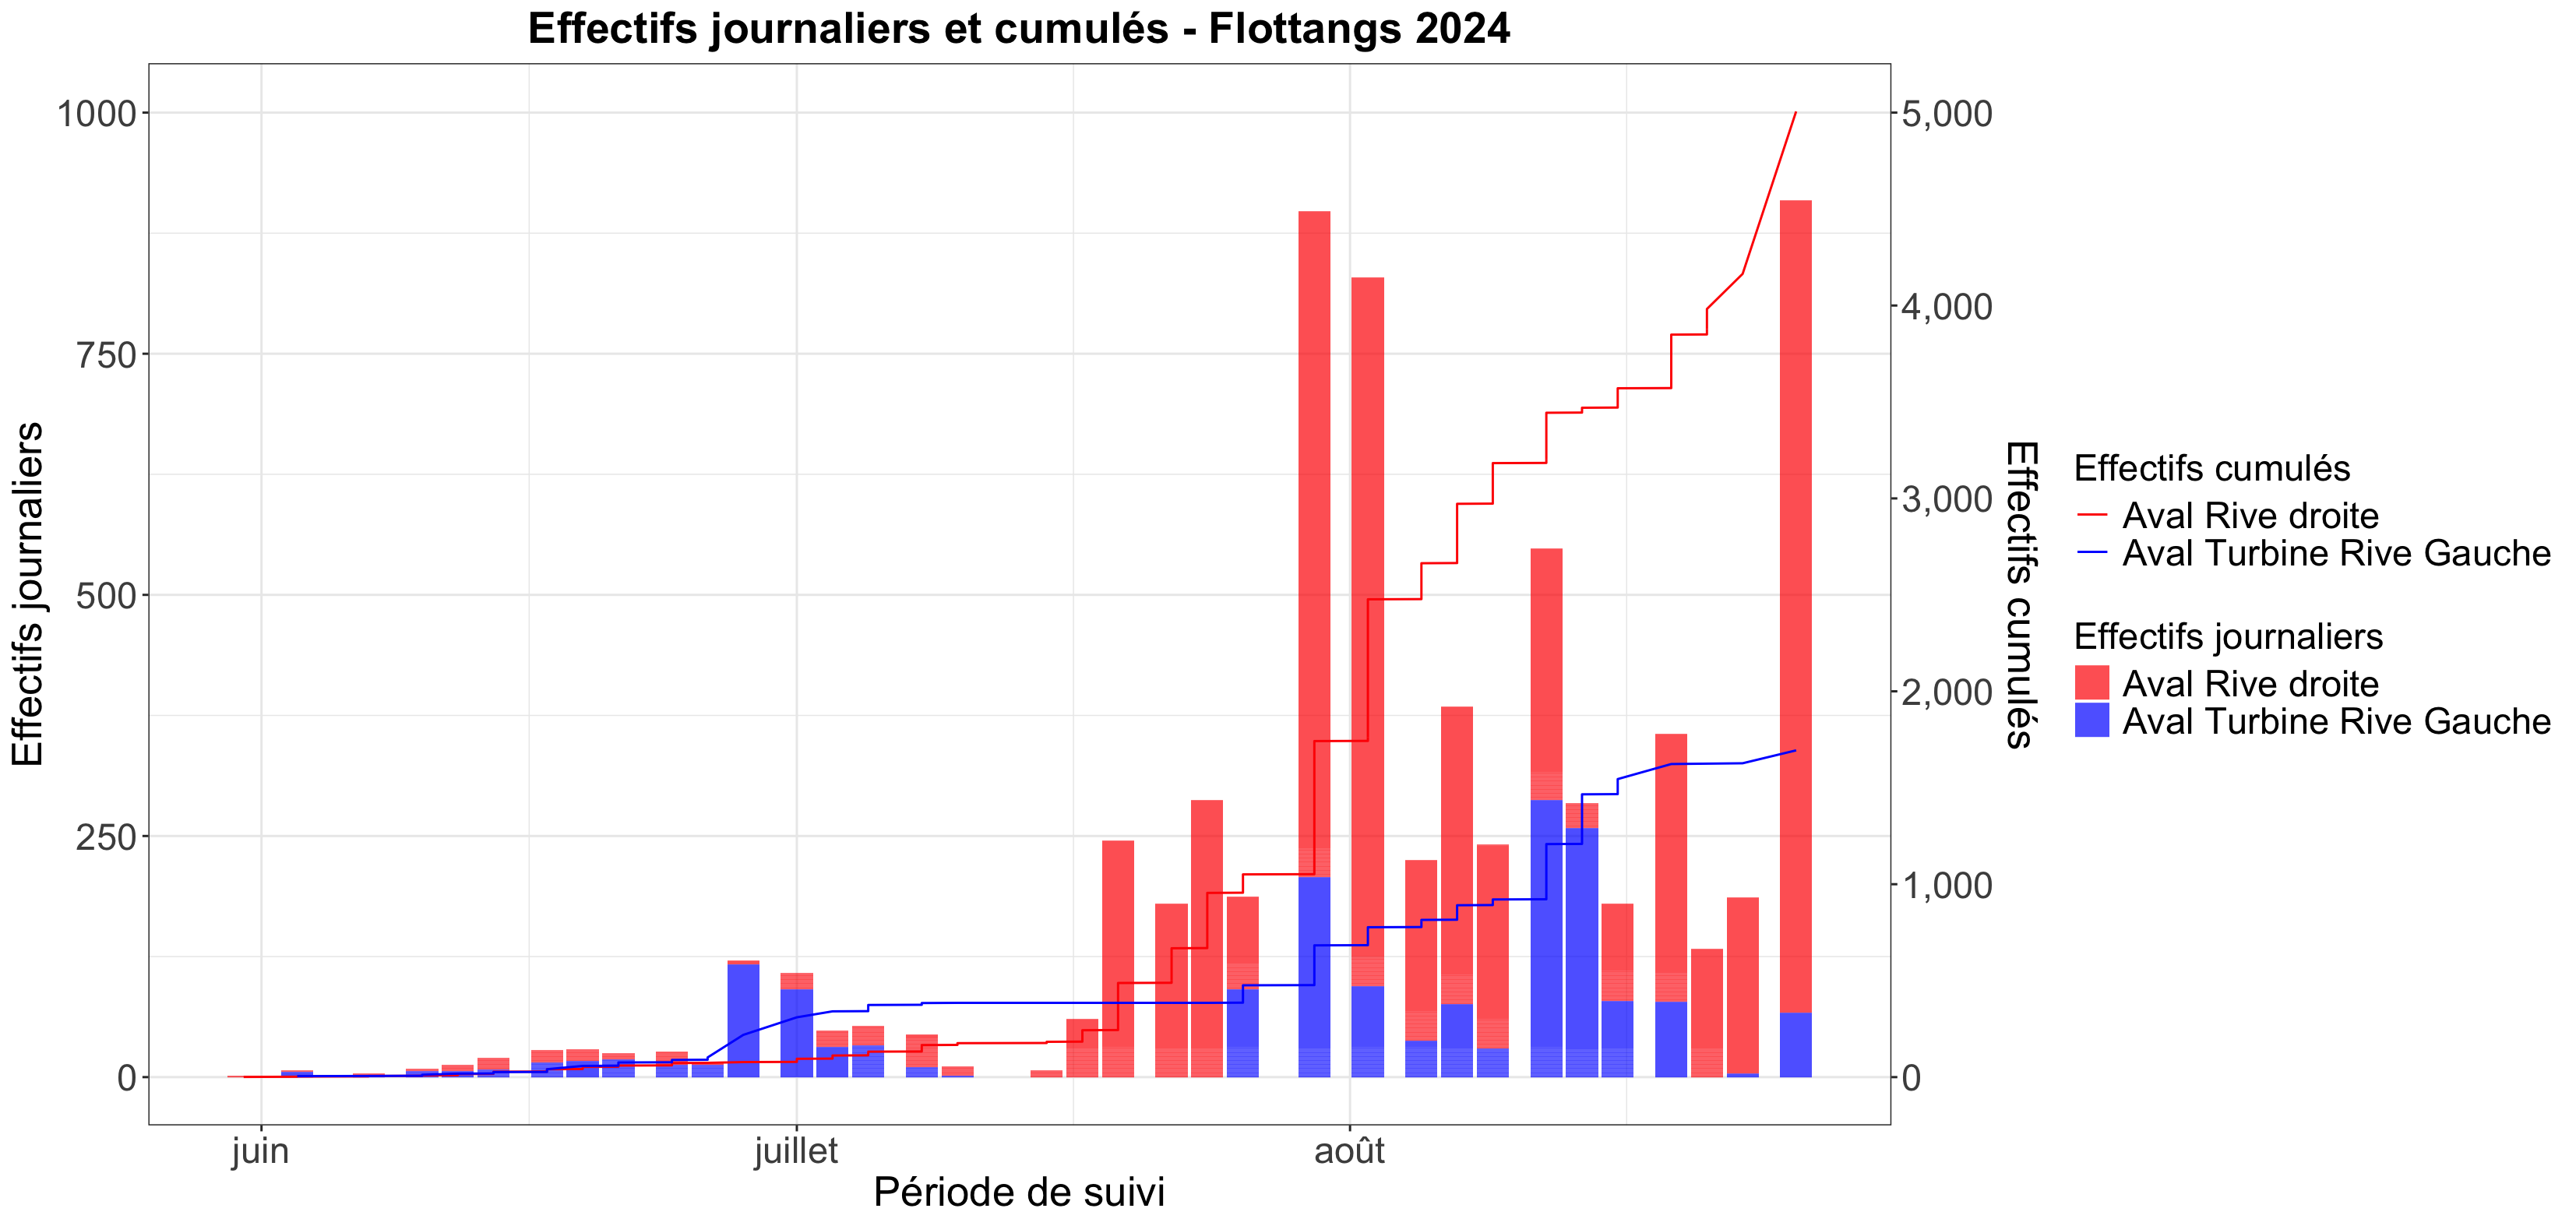
\includegraphics[width=\textwidth]{graph_flottang_oral.png}
\caption{Effectifs cumulés et journaliers des flottangs AVR et AVT 2024}
\label{graph_flottang_oral}
\end{figure} 

\subsubsection{Tailles des individus}

La (Figure \ref{taille_flottang_oral}) présente la taille des individus en mm dans les flottangs. Nous pouvons voir que la majorité des individus retrouvés dans le flottangs AVR mesurent entre 70 et 80 mm ce qui correspond aux individus de l’année. Dans le flottang AVT une majorité d’individus sont des anguilles de l’année mais il y a aussi une distribution des individus de toutes tailles allant de 100 mm jusqu’à 175 mm. Pour le flottang AVT la taille moyenne est de 95.7 mm avec une médiane de 82 mm alors quand rive droite la taille moyenne des individus est de 87.9 mm avec une médiane a 79 mm. Les individus observés dans le flottang AVT sont significativement plus grands que ceux observés dans le flottang AVR (wilcox-test, p < 0,05). Ce résultat est contraire au résultat obtenu pour la taille des individus retrouvés dans les pièges en rive droite et en rive gauche.

\begin{figure}[htpb]
\centering
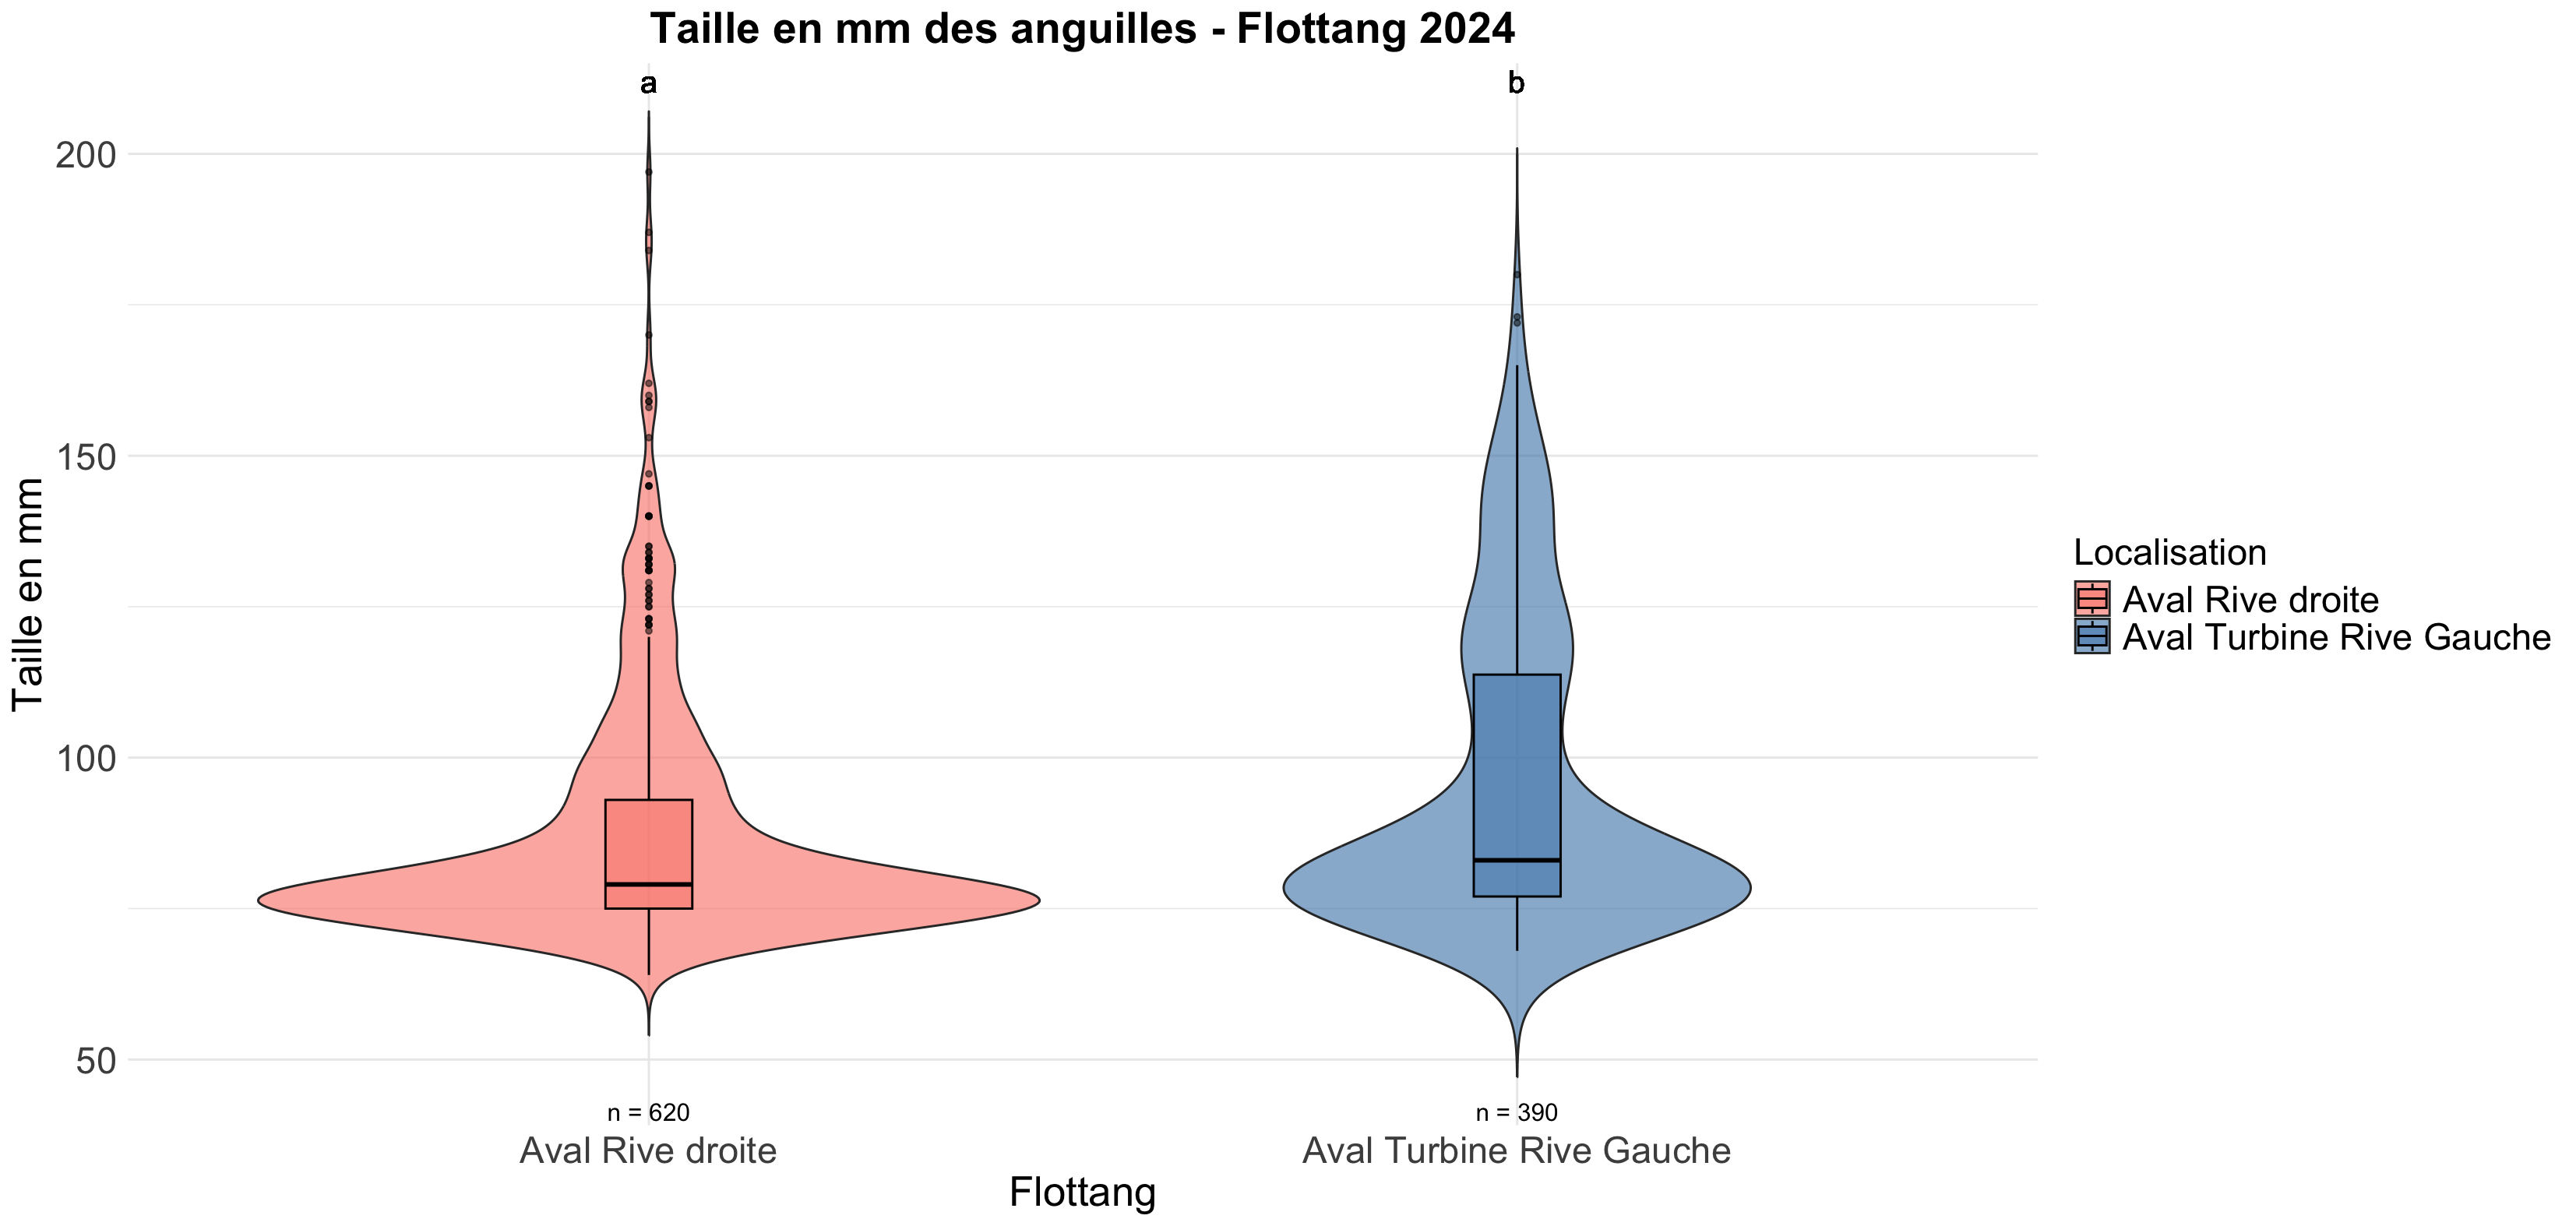
\includegraphics[width=\textwidth]{taille_flottang_oral.png}
\caption{Taille en mm des anguilles observées dans les flottangs AVR et AVT}
\label{taille_flottang_oral}
\end{figure} 

\subsubsection{État sanitaire }

Au total 6.21\% (59/950) des anguilles biométrées ont des lésions Tableau \ref{tableau 4}. Le calcul d’IpG montre une condition des poissons \og Bonne \fg{} et le calcul d’IpP montre une condition des poissons \og excellente \fg{}.  Les pathologies le plus souvent retrouvée sur les anguilles sont les lésions majeures avec 51\% puis 32\% de parasitisme et 17\% de lésions mineurs. Si nous traitons la rive droite et la rive gauche séparément les calculs des indices pathologiques montrent une condition des poissons \og bonne \fg{} à la fois pour la rive gauche et pour la rive droite. Les calculs d’indice parasitaire donnent les mêmes résultats que pour les deux rives confondues avec une condition des poissons \og excellente \fg{}. La distribution des catégories pathologiques est assez similaire avec seulement un pourcentage de parasitisme plus élevé en rive gauche avec 38\%, un pourcentage de lésions majeurs plus faibles avec 41\% et un pourcentage de lésions mineures plus élevés avec 21\%. Cette proportion plus importante d’anguilles ayant une pathologie de types parasites en AVT est la même que celle retrouvée en rive gauche. Au total 8 pathologies ont été observées sur les anguilles dont 2 issues de parasites, les points noirs et les points blancs. Les pathologies les plus retrouvées chez les individus sont la présence de points noirs (27\%) et la présence de marques d’érosion (25\%). Ensuite, la présence d’hémorragie est retrouvée à 17\% et la présence de plaie retrouvé à 14\%.


\begin{table}[h!]
\centering
\begin{tabular}{|c|c|c|c|} 
\hline
  & RG  & RD & RG+RD\\ [0.5ex] 
 \hline
 Nombres de poissons examinés & 390 & 560  & 950 \\ 
 \hline
 Nombres de poissons avec pathologies  & 29  & 30 & 59 \\
 \hline
 IpG & \textcolor{green}{0.09} & \textcolor{green}{0.10} & \textcolor{green}{0.18}\\
 Condition des poissons & Bonne &  Bonne  & Bonne\\
 \hline
 IpP & \textcolor{blue}{0.03} & \textcolor{blue}{0.01} & \textcolor{blue}{0.02}\\ [0.5ex] 
 Condition des poissons & Excellente & Excellente  & Excellente\\
 \hline
 Parasitisme & 38\%  & 27\% & 32\%\\
 Lésions majeures & 41\%  & 60\% & 51\%\\
 Lésions mineures  & 21\% &  13\%  & 17\%\\ [1ex] 
 \hline
 
\end{tabular}
\caption{Synthèse de l’état sanitaire dans les flottangs AVR et AVT 2024}
\label{tableau 4}
\end{table}

\section{Discussion}

L’année 2024 est la 11ème année en rive gauche et 7ème année en rive droite que le suivi du recrutement de la Seine en anguille européenne est réalisé sur le barrage de Poses. Durant la période de suivi, du 2 avril au 23 septembre, 846 545 anguilles ont été observées dans les pièges dont 85 017 anguilles en rive droite et 761 528 en rive gauche. Cette préférence pour la rive droite est cette année encore bien marquée. Deux gros pics de migration d’anguilles ont eu lieu durant la période de suivi, la première du 27 juillet au 2 août pendant lequel 125 475 anguilles ont été observées (les deux rives confondus). Le second pic le plus important à eu lieu du 9 au 16 août pendant lequel 303 037 anguilles ont été observées. Au total durant ces deux pics 428 504 anguilles sont passées dans les pièges ce qui correspond à 50\% des individus observés sur la durée totale du suivi. 

\vspace{0.5cm}
Cette année est la meilleure depuis le début des suivis pour la rive droite car le total de 476 958 anguilles en 2018 est dépassé. Ce constat est le même pour la rive gauche car la meilleure année était 2022 avec 36 046 est lui aussi dépassé. 

\vspace{0.5cm}
Cette année les premiers individus ont pu être observés le 8 avril pour les deux rives. Durant les mois d’avril, mai et juin les anguilles observées dans les pièges étaient des anguilles en reprise de migration c’est-à-dire des anguilles qui ont déjà au moins passé une année dans l’estuaire, leur taille étaient de 100 mm jusqu’à 300 mm. Ce n’est quand juillet que les premiers individus de l’année ont été observés avec une taille inférieure à 80 mm. Pour la première fois depuis le début des suivis en 2014, en rive gauche de nombreux individus de l’année ont pu être observés. Le pourcentage d’individus de l’année est même plus élevé en rive gauche avec 42\% des effectifs contre 30\% en rive droite. Ce changement est important à relever car depuis 2014 le dispositif en rive gauche présente une certaine sélectivité sur les petits individus. La récolte de données depuis quelques années a mis en avant une mauvaise condition d’accessibilité de la rampe en rive gauche. Cela est dû au fait que l’usine hydroélectrique génère de forts courant qui masquent l’attractivité de la rampe. De plus les forts courants viennent s’ajouter à la difficulté car les jeunes anguilles ont une nage très limitée. La présence de palplanches en berge vient aussi empêcher les anguilles d’avoir des points de fixation, de repos lors de la montaison (Figure \ref{Discu}). 

\begin{figure}[htpb]
\centering
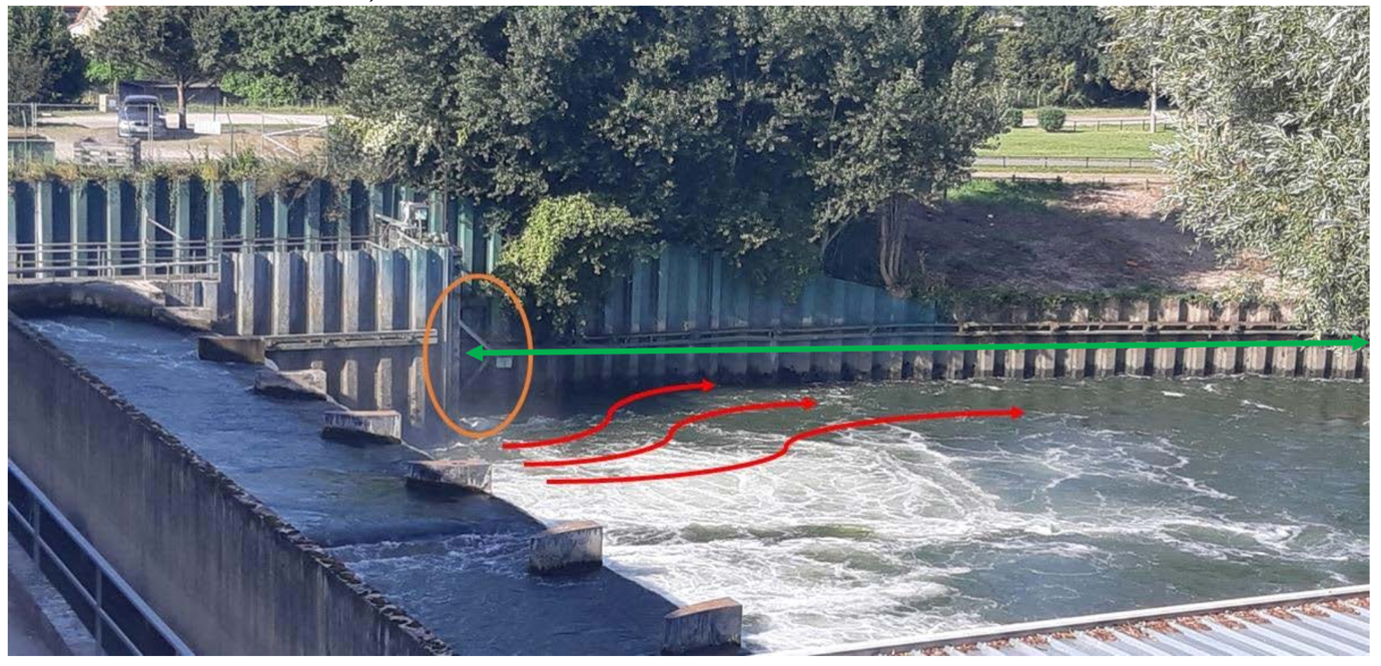
\includegraphics[width=\textwidth]{Discu.png}
\caption{Photographie de l’aval de la centrale hydroélectrique et de la rampe à anguille (orange) en rive gauche. En vert, les palplanches longeant la berge et en rouge les courants limitants la montaison (Adapté de Théo Neveu, 2021).}
\label{Discu}
\end{figure} 

\vspace{0.5cm}
Cette année l’explication de l’observation de nombreux individus de petites tailles dans le piège rive gauche semble être le très fort débit enregistré pendant toute la période du suivi qui a permis d’avoir un niveau d’eau en aval du barrage plus élevé que les années précédentes (Figure \ref{graph_debit_oral}). Ce niveau d’eau plus élevé semble être venu contrer les forts courants produit par l’usine hydroélectrique en aval du dispositif et a permis aux anguilles d’atteindre plus facilement l’entrée de la rampe avec un peu moins de difficulté comparée aux années précédentes. En rive gauche, les années ayant eu des débits élevés sont les années où un nombre conséquent d’anguilles ont été observées dans le piège (2022, 2018 et 2016). Seule l’année 2021 a eu des débits plus élevés durant les mois de juillet et août que l’année 2024 ; cependant aucune comparaison ni corrélation ne peuvent être faites sur l’influence des débits sur les courants produits par l’usine hydroélectrique car durant l’été 2021 le piège en rive gauche a eu un dysfonctionnement de pompe.

\vspace{0.5cm}
Pour la rive droite les chiffres d’individus de l’année sont similaires aux années précédentes. A noté que ce dispositif est lui aussi imparfait. Le débit d’attrait en aval du dispositif est jugé insuffisant.  L’attrait est généralement compris entre 4 à 4,2 m3/s, alors qu’un attrait de 4,1 à 6,7 m3/s serait plus adapté pour les anguilles (d’après l’expertise de SCIMABIO Interface et OTEIS). L’attractivité du dispositif pourrait être encore amélioré avec la mise en route de la vanne de régulation. Des études ont été faites pour montrer que monter la vanne permettrait d’augmenter la vitesse d’écoulement et donc favoriser l’attraction.

\vspace{0.5cm}
Depuis le début des suivis chaque année l’état sanitaire est très bon. Cette année les calculs d’indice pathologique globale et d’indice parasitaire continuent d’être dans la même tendance. Les conditions des poissons sont excellentes au niveau parasitaire sur les deux rives ainsi que pour les flottangs. L’indice pathologiques globale donne une condition des poissons bonne pour la rive gauche et les flottangs et précaire pour la rive droite. Au total sur 5419 individus biométrés (les deux rives et les deux flottangs confondus) 533 anguilles présentent une pathologie (10.2\%). La nature pathologique la plus retrouvée est la lésion majeure avec 58\% suivi par le parasitisme avec 28\% et la nature pathologique la moins rencontrée est la lésion mineure avec 14\%.

\vspace{0.5cm}
En comparaison avec les années précédentes, la nature pathologique la plus rencontrée est différente. Le parasitisme était dominant sur les deux autres natures pathologiques. Cette année les individus touchés par un parasite ne sont que de 28\%.  D’après \citep{elie_sante_2014}, différents facteurs peuvent jouer un rôle sur le nombre de pathologies rencontrées. Particulièrement la température de l’eau augmenterait la rapidité de déroulement des cycles parasitaires. En \citep{lafferty_how_1999},  dit aussi que les effluents thermiques diminuent les capacités immunitaires de l’hôte et donc favorisent le parasitisme. Les courants lents ainsi que les hydrosystèmes à faciès lenthiques augmenteraient la présence de parasites dans les systèmes aquatiques \citep{berra_incidence_1978,janovy_evolutionary_1997}. En aval du barrage de Poses, les hydrosystèmes sont eux lotiques, les courants sont généralement forts car soumis au phénomène de marée et cette année les forts débits peuvent avoir un lien avec le plus faible taux de parasitisme rencontré sur les individus. La présence de points noirs a été observés davantage chez des individus de l’année car leur peau n’est pas encore assez épaisse. D’après \citep{elie_sante_2014}, en raison de l’épaisseur de sa peau l’anguille n’est pas affectée.  

\vspace{0.5cm}
La pathologie la plus observées sur les individus est la présence d’érosion. En grande proportion, les anguilles présentant des érosions étaient des individus ayant déjà passé au moins une année en estuaire, très peu d’individus de l’année présentaient des érosions. Les causes principales d’érosion étant les frottements durant la migration mais aussi éventuellement des parasites externes ou des carences \citep{elie_sante_2014}.  

\vspace{0.5cm}
La montaison des anguilles est influencée par différents facteurs environnementaux. D’après des études de \citep{white_environmental_1997} la température de l’eau fortement corrélée à la température de l’air serait le déclenchement de la montaison et particulièrement lorsque la température de l’eau se situerait entre 12 et 14°C. D’après \citep{adam_anguille_2008}. La température de l’air ainsi que la température de l’eau jouent un rôle au niveau des dispositifs à anguilles. Les premières anguilles ont été capturées à la suite de la mise en route des dispositifs. À cette date de lancement, le 2 avril la température de l’eau était de 12.3°C, ce qui est en lien avec la littérature où la montaison se déclenche entre 12 et 14°C \citep{white_environmental_1997}. Certaines autres années, les premières anguilles pouvaient être observées deux semaines après le lancement du dispositif à la mi-avril. Ce constat était rencontré quand la température de l’eau était inférieure à 12°C début avril.

\vspace{0.5cm}
En \citep{hirschinger_donnees_2015} a montré que des forts débits peuvent avoir un impact sur la montaison des anguilles. Les débits peuvent ralentir ou même bloquer la migration des civelles. Cette année les mois d’avril et mai ont eu des débits forts, les individus que nous avons observé dans les pièges était des individus de plus d’une année et aucune civelle n’a été observée durant ces mois-ci. Néanmoins aucune corrélation significative n’a été mise en évidence en 2024. Les coefficients de marée et les débits n’ont eux aussi aucune corrélation significative. Ce résultat est contraire à la littérature car des études ont montré que les coefficients de marée avaient une corrélation avec la migration des anguilles. \citep{gascuel_flow-carried_1986, elie_migration_1994}. Les études sur l’influence des coefficients de marée ont été faites proches de la mer contrairement au barrage de Poses (160km de la mer) ce qui peut expliquer des résultats contradictoires.  Cependant, les ressentis terrain était eux similaires car les jours ayant eu le plus d’anguilles dans les pièges n’étaient pas des jours à forts coefficient de marée. Inversement, aucun pic d’anguille n’a été observé les jours avec des forts coefficients de marée. Cette année, le cycle lunaire n’a pas été étudié mais d’après certaines études il pourrait exercer une influence sur la migration lors de nouvelle lune \citep{casamajor_fluctuations_2001}.

\vspace{0.5cm}
Le suivi flottangs a été réalisé pour la 10ème fois cette année, comme dit plus tôt les flottangs ont été mis en place plus tard comparé aux années précédentes dû au trop haut niveau de l’eau en aval des dispositifs. Ce suivi vient en complémentarité avec le suivi des passes à anguilles. En 2018, MIGADO a montré que ce dispositif de flottangs pouvait mettre en évidence un effet d’accumulation en aval des passes à anguilles \citep{lauronce_actions_2018}. Les années précédentes, un flottang était mis en place en amont des écluses rive droite. Il a permis de mettre en évidence le passage des anguilles par les écluses mais pas de quantifier car un seul flottang sous-estime énormément le nombres d’anguilles empruntant les écluses. Cette année ce flottang a été placé en aval du dispositif en rive gauche AVT tout comme en rive droite (AVR). 

\vspace{0.5cm}
Au total, 6702 anguilles ont été relevée dans les flottangs ce qui est un très faible nombre comparé aux anguilles retrouvées dans les pièges. Les jours ou les effectifs d’anguilles présentent dans les flottangs étaient le plus élevé correspond aux jours durant lequel nous avons constaté les pics de migration dans les cuves. Aucune accumulation d’anguille au pied des dispositifs semble être mis en évidence. Les flottangs sont utilisés par les anguilles comme une zone de repos durant leur montaison à la fois en rive gauche et en rive droite. 

\vspace{0.5cm}
Une hypothèse est que les individus se reposent dans les flottangs en attendant les marrées hautes pour faciliter leur passage dans les dispositifs. Cette hypothèse peut être avérée en rive gauche avec l’absence totale d’autres zone de repos à cause des palplanches et des vitesses de courants forts avec l’usine hydroélectrique. Une seconde hypothèse est le fait que les anguilles peuvent arriver dans la journée au pied du dispositif et attendent la nuit pour entamer leur montaison sur la passe. La nuit est plus favorable à la progression sur les rampes pour les anguilles car elles ne sont pas exposées à la lumière et surtout au soleil qui peut être fort en plein été mais aussi pour éviter les prédateurs. 

\vspace{0.5cm}
\textbf{Limite et biais}
 

Cette année il est important de noter qu’aucun dysfonctionnement n’a été rencontré. La montaison des anguilles s’est déroulée sans impact significatif des problèmes de rampes qui peuvent engendrer de la prédation au pied des passes ou même de la mort à cause de la fatigue en ne trouvant pas l’entrée de la rampe.

\vspace{0.5cm}
Pour le tamisage, une maille de 6 mm est utilisée. Cette maille permet de laisser passer des individus supérieurs à 120 mm alors que cette opération au préalable est effectuée pour séparer les individus de l’année et les individus plus gros lors des relèves pour ensuite faire de la biométrie sur des échantillons des deux groupes. L’estimation du nombre d’individus dans le piège lors des relèves est faite sur la base des individus sur lequel la biométrie est faite (environ 60 individus par relève). Ce faible nombre pris aléatoirement ne représente pas toujours la réalité, c’est pourquoi en parallèle environ 200 individus sont comptés et pesés afin d’obtenir des poids qui représentent la totalité des anguilles pour une estimation plus précise. De plus la balance avec laquelle nous pesons les anguilles ne garantit pas des données optimales. Elle est aussi sensible à l’eau, au vent et il est possible que l’opérateur lors des pesées ajoute de l’eau ce qui peut entrainer un biais sur le poids des petits individus. Sa précision au dixième de grammes n’est pas suffisante pour les individus de l’année qui ont un poids entre 0.2 et 0.8 g. Même si toutes les précautions ainsi qu’un maximum d’application lors des mesures sont faites, les données de poids ne sont pas fiables à 100\%. C’est pour cela que la partie résultats traite la taille et non le poids des individus.

\vspace{0.5cm}
Le recrutement de l’anguille européenne réalisé sur le barrage de Poses est sûrement sous-estimé avec les pièges car nous savons que les écluses sont une voie de passage lors de la montaison des anguilles. Cependant aujourd’hui encore aucune méthode n’a été mise en place pour pouvoir quantifier le nombre d’anguille empruntant les écluses ce qui permettrait d’avoir le recrutement total d’anguille.
Les flottangs pour la relève doivent être remontés de l’eau sur le sol depuis la berge. Lors de cette méthode de relevé nous avons vu que quelques anguilles présentes dans le flottang tombent et s’échappent. Il semble donc que les captures des flottangs soient eux aussi un peu sous-estimées. Cela est valable pour l’AVT en rive gauche et l’AVR en rive droite.

\vspace{0.5cm}
De nombreux problèmes émis dans ce rapport devraient être résolus pour pourvoir permettre aux anguilles de réaliser une montaison optimale sur le barrage. En rive droite, le principal problème est le débit d’attrait trop faible. Comme dit précédemment, des expertises sont en cours mais rien n’a encore était fait. En rive gauche, le principal problème est la difficulté pour les anguilles d’arriver sur la rampe à cause des courants produits par l’usine électrique et l’absence de zone de repos à cause des palplanches. Peut-être qu’une mise en place de divers supports ou de zone de repos serait possible, comme réaliser un enrochement mais la réalisation est complexe.

\vspace{0.5cm}
Pour résumé, cette étude du recrutement de l’anguille montre bien la difficulté des individus d’atteindre les rampes construites pour faciliter leur montaison. Le barrage de Poses est le premier ouvrage sur la Seine avant de nombreux autres obstacles. Sur l’axe Seine seul l’ouvrage situé au-dessus de Poses est équipé d’une rampe à anguille. Les ouvrages suivants possèdent uniquement des passes à poissons car ceux-ci se trouvent en dehors de la ZAP anguille. Au vu de l’importance de cet axe pour les anguilles, chaque ouvrage devrait être équipé de rampe à anguille. Les données mettent en lumière le besoin d’amélioration et d’optimisation aux niveaux des dispositifs mais aussi les influences que peuvent avoir les différents facteurs environnementaux sur la montaison ainsi que sur les pathologies de types parasitisme. Bien que cette année soit la meilleure année en termes de nombres d’anguilles depuis le début des suivis, ce nombre est encore bien loin des chiffres des années 80 ou l’anguille n’était pas encore en danger critique d’extinction. De nombreuses actions doivent encore être réalisées pour continuer à préserver les populations d'anguille européenne.

\section{Conclusion}

L’anguille européenne était abondante dans les eaux européennes, et même classée nuisible jusqu’en 1984. Les populations ont ensuite drastiquement diminué depuis le milieu du XXème siècle. Son statut a évolué au fur et à mesure du temps passant de \og vulnérable \fg{} puis \og en danger \fg{} pour être \og en danger critique d’extinction \fg{} aujourd’hui. Pour stopper ce déclin et maintenir les populations d’anguille, la commission européenne exige à chaque état membre l’élaboration d’un plan de gestion national (PGA), décliné localement en unités de gestion (UGA). Sur le barrage de Poses, un suivi du recrutement d’anguille européenne a été mis en place car il est le premier obstacle depuis la mer. Cette année 2024, du 2 avril au 23 septembre un total de 846 545 anguilles ont été observées dans les pièges dont 85 017 anguilles en rive droite et 761 528 en rive gauche. Ce sont les meilleurs chiffres obtenus depuis le début des suivis à la fois en rive droite et en rive gauche. La rampe en rive droite, plus adapté au passage des anguilles a été plus utilisé par rapport à la rive gauche. Sur le plan sanitaire, la tendance des conditions des anguilles continue d’être excellente pour l’indice parasitaire et bonne pour l’indice pathologique globale. Au total, 10,6\% des anguilles biométrées (474/4469) présentent des pathologies. L’influence positive des températures sur la montaison des anguilles a pu cette année encore être mise en évidence. Les flottangs n’ont pas mis en évidence d’accumulation au pied des rampes et l’état sanitaire des individus est similaire aux individus retrouvés dans les pièges. Malgré les bons résultats obtenus cette année de nombreuses améliorations doivent être mise place pour optimiser la montaison des anguilles et plus particulièrement des jeunes individus. Ce suivi du recrutement est sûrement légèrement sous-estimé car nous savons que les écluses sont une voie de passage. Une mise en place d’un dispositif de comptages au niveau des écluses serait très intéressante pour avoir des chiffres très proche de la réalité des effectifs totaux franchissant le barrage de Poses.

\vspace{0.5cm}
Cette année, malgré le meilleur chiffre de montaison observé sur le barrage de Poses depuis le début des suivis, cela ne nous permet pas de qualifier la situation de satisfaisante même si une amélioration est visible. Sur le plan national, avec les données d’autres associations migrateurs le recrutement sur la Seine semble suivre la tendance. L’année 2024 semble être une bonne année de recrutement de l’anguille sur les principaux fleuves français.

% Ajouter la section Références dans la table des matières
\addcontentsline{toc}{section}{Références}


%\twocolumn
% biblio commune aux différentes années
\bibliographystyle{apalike}
\bibliography{Biblio_M2}
\normalsize
\null
\vfill

\end{document}
